%%	SECCION documentclass																									 %%	
%%---------------------------------------------------------------------------%%
\documentclass{article}

%%---------------------------------------------------------------------------%%
%%	SECCION usepackage																											 %%	
%%---------------------------------------------------------------------------%%
\usepackage{amsmath, amsthm}
\usepackage[spanish,activeacute]{babel}
\usepackage{caratula}
\usepackage{a4wide}
\usepackage{hyperref}
\usepackage{fancyhdr}
\usepackage{dsfont}
% \usepackage{moreverb}
\usepackage{graphicx} % Para el logo magico!
\usepackage{capt-of}
\usepackage{afterpage}
\usepackage{float}
\usepackage{amssymb}
\usepackage{amsmath}
\usepackage[latin1]{inputenc}
\usepackage{subfigure}
\usepackage{algorithm}
\usepackage{algorithmic}
\usepackage[dvipsnames,usenames]{color}
\usepackage{amsfonts}
\usepackage{code_color}
\usepackage{amsthm}
\usepackage{marvosym}
%\usepackage{minipage}

%%---------------------------------------------------------------------------%%
%%	SECCION opciones																												 %%	
%%---------------------------------------------------------------------------%%
\parskip    = 11 pt
\headheight	= 13.1pt
\pagestyle	{fancy}
\definecolor{orange}{rgb}{1,0.5,0}

\addtolength{\headwidth}{1.0in}

\addtolength{\oddsidemargin}{-0.5in}
\addtolength{\textwidth}{1.0in}
\addtolength{\topmargin}{-0.8in}
\addtolength{\textheight}{0.7in}

%%%---------------------------------------------------------------------------%%
%%%	SECCION listings    													 %%	
%%%---------------------------------------------------------------------------%%
%\usepackage{listings}
%\lstset{
%		language=C++,
%		basicstyle=\ttfamily \small,
%		keepspaces=true,
%		flexiblecolumns=false,
%		basewidth={0.5em,0.45em},
%		keywordstyle=\ttfamily \bfseries \hlkwa,
%		tabsize=4
%}

\newcommand{\Nat}{\mathbb{N}}
\newcommand{\Int}{\mathbb{Z}}
\newcommand{\Real}{\mathbb{R}}
\newcommand{\tq}{\ensuremath{\,|\,}}
\newcommand{\imp}{\ensuremath{\Rightarrow}}

%%---------------------------------------------------------------------------%%
%%	SECCION document	 %%	
%%---------------------------------------------------------------------------%%
\begin{document}
\renewcommand{\chaptername}{Parte }
\renewcommand{\algorithmicrequire}{\textcolor{blue}{\textbf{Requiere:}}}
\renewcommand{\algorithmicensure}{\textbf{Devuelve:}}
\renewcommand{\algorithmicend}{\textbf{Fin}}
\renewcommand{\algorithmicif}{\textcolor{blue}{\textbf{Si}}}
\renewcommand{\algorithmicthen}{\textcolor{blue}{}} %%\textbf{entonces}}}
\renewcommand{\algorithmicelse}{\textcolor{red}{\textbf{Si no}}}
\renewcommand{\algorithmicelsif }{\textcolor{blue}{\textbf{Si no y}}}
\renewcommand{\algorithmicendif}{\textcolor{blue}{\textbf{Fin si}}}
\renewcommand{\algorithmicfor}{\textcolor{ForestGreen}{\textbf{Para}}}
\renewcommand{\algorithmicendfor}{\textcolor{ForestGreen}{\textbf{Fin para}}}
\renewcommand{\algorithmicwhile}{\textcolor{ForestGreen}{\textbf{Mientras}}}
\renewcommand{\algorithmicendwhile}{\textcolor{ForestGreen}{\textbf{Fin mientras}}}
\renewcommand{\algorithmicdo}{\textcolor{ForestGreen}{}} %%\textbf{hacer}}}
\renewcommand{\algorithmicreturn}{\textbf{Devolver}}
\floatname{algorithm}{Algoritmo}

%%---- Caratula -------------------------------------------------------------%%
\materia{Problemas, algoritmos y programaci�n (2010)}
\titulo{Trabajo Pr'actico n� 4}


\integrante{Barenbaum, Pablo}{124/04}{foones@gmail.com}
\integrante{Mart'inez, Federico}{17/06}{federicoemartinez@gmail.com}
\integrante{Sainz-Tr'apaga, Gonzalo}{454/06}{gonzalo@sainztrapaga.com.ar}
\grupo{Grupo 1}
\resumen{
El siguiente informe presenta la resoluci�n a los 4 problemas correspondientes al cuarto trabajo pr\'actico de la materia Problemas, Algoritmos y Programaci�n en el primer cuatrimestre del 2010. En el mismo se encuentra la explicaci�n del algoritmo utilizado para resolver cada problema, as� como tambi�n la implementaci�n en C++ de los mismos.
}

% TOC, usa estilos locos
\maketitle
\pagestyle{empty}
{
\fancypagestyle{plain}
    {
    \fancyhead{}
    \fancyfoot{}
    \renewcommand{\headrulewidth}{0.0pt}
    } % clear header and footer of plain page because of ToC
%\tableofcontents
}

\newpage
% arreglos los estilos para el resto del documento, y
% reseteo los numeros de pagina para que queden bien
\pagenumbering{arabic}
\fancypagestyle{plain} {
    \fancyhead[LO]{Barenbaum, Mart�nez, Sainz Tr�paga}
    \fancyhead[C]{}
    \fancyhead[RO]{P\'agina \thepage\ de \pageref{LastPage}}
    \fancyfoot{}
    \renewcommand{\headrulewidth}{0.4pt}
}
\pagestyle{plain}
\newcommand{\cosito}[0]{\textcolor{Orange}{\huge$\cdot$}}
\section{4289 - Disgruntled Judge}
\textbf{Problema:}
Dada una sucesi�n de n�meros $x_1, x_3, ... , x_{2t-1}$, encontrar $x_2, x_4, ... , x_{2t}$, tal que:
$$\exists a, b \in \mathds{Z}, 0 \leq a,b \leq 10000, \forall 0 \leq i \leq 2t-1, x_{i+1} = a* x_{i} + b \mod 10001$$ 

\subsection{Resoluci�n}
Para resolver el problema primero notamos que $10001 = 73*137$, lo cual puede ser �til para aplicar el teorema chino del resto. 
Llamaremos $I_{i} = x_{2i-1}$ y $O_{i} = x_{2i}$. Notemos que como el enunciado nos dice que $0 \leq x_{i} \leq 10000$, resulta que los $x_{i}$ son restos de la divisi�n m�dulo 10001. Esto resulta importante porque nos permite trabajar con congruencia en vez de igualdad.

Si el \textit{input} es s�lo $I_1$, alcanza con tomar $O_1=I_1$, pues se puede tomar $a=0, b=I_1$. An�logamente, si el \textit{input} es s�lo $I_1, I_2$, alcanza con tomar $O_k = I_2$, pues se puede usar $a=0, b = I_2$.

Si la cantidad de \textit{inputs} ($n$) es mayor, hay que plantearlo de otra forma. 

Consideremos un caso tal que la cantidad de \textit{inputs} es mayor o igual a 3. Observando las ecuaciones de generaci�n de los $x_i$ vemos que:

$$a*I_1 + b \equiv O_1 \mod 10001$$
$$a*0_1 + b \equiv I_2 \mod 10001$$
$$a*I_2 + b \equiv O_2 \mod 10001$$
$$a*O_2 + b \equiv I_3 \mod 10001$$

De aqu� podemos obtener:

$$a^2*I_1 + a*b + b \equiv I_2 \mod 10001$$
$$a^2*I_2 + a*b + b \equiv I_3 \mod 10001$$

Restando ecuaciones,

$$a^2*(I_1 - I_2) \equiv (I_2 - I_3) \mod 10001$$

Resolviendo esta ecuaci�n podemos obtener candidatos para $a^2$, y de estos candidatos podemos obtener posibles valores para $a$.

Notemos que si $(I_1 - I_2)\equiv 0 \mod 10001$, resulta que $I_1 = I_2$, ya que $0 \leq I_1,I_2 \leq 10001$. %TODO: lo explico mas esto?
En ese caso, alcanza con devolver $O_k=I_2$

Usando teorema chino del resto, obtenemos que:
$$a^2*(I_1 - I_2) \equiv (I_2 - I_3) \mod 137$$
$$a^2*(I_1 - I_2) \equiv (I_2 - I_3) \mod 73$$

Supongamos que $(I_1 - I_2) \not\equiv 0 \mod 137 \wedge (I_1 - I_2) \not\equiv 0 \mod 73$
Entonces, como ambos m�dulos son primos, existen $k_{73}, k_{137}$ inversos multiplicativos de $(I_1 - I_2)$ m�dulo 73 y 137 respectivamente, tales que:
$$a^2 \equiv (I_2 - I_3)*k_{137} \mod 137$$
$$a^2 \equiv (I_2 - I_3)*k_{73} \mod 73$$

Para encontrar los $k$ se busca expresar a 1 como combinaci�n lineal entre $(I_1 - I_2)$ y 137 o 73 seg�n corresponda, lo cual es posible, ya que estamos suponiendo que $(I_1 - I_2)$ es coprimo con 137 y con 73.

Luego buscamos $a$ tales que $a^2$ cumpla esas ecuaciones. Si $(I_1 - I_2) \equiv 0 \mod 137 \vee (I_1 - I_2) \equiv 0 \mod 73$ (es un ``o'' exclusivo, porque estamos considerando que no $(I_1 - I_2)$ no era m�ltiplo de $10001$), perdemos una de las ecuaciones, pero igual obtenemos posibles candidatos para $a^2$.

Una vez que obtenemos un candidato para $a$, vemos si es viable. Para esto debe ser posible encontrar $b$ tal que:
$$a^2*I_1 + a*b + b \equiv I_2 \mod 10001$$
Escrito de otra forma:
$$(a+1)*b \equiv I_2 - a^2*I_1 \mod 10001$$

Un caso donde podr�a no existir ning�n $b$ que cumpla esta ecuaci�n es si  $(a+1) \equiv 0 \mod 10001$, pero el lado derecho de la ecuaci�n no es equivalente a 0. Usando teorema chino del resto, se obtienen dos ecuaciones m�dulo 173 y 73, que permiten obtener un $b$ candidato. 
En verdad no puede ser que $(a+1) \equiv 0 \mod 10001$, porque entonces resulta que $a^2 \equiv 1 \mod 10001$ y de $(a+1)*b \equiv I_2 - a^2*I_1 \mod 10001$ sale que $I_1 \equiv I_2 \mod 10001$, pero ese caso yo lo hab�amos considerado antes por separado. 
Sin embargo, si puede ocurrir que $(a+1) \equiv 0 \mod 73$ o $(a+1) \equiv 0 \mod 137$ y que no valga que el lado derecho tambi�n sea congruente a 0, por lo cual hay que chequear esas condiciones.

Dado un valor de $k\neq 0$, existen a lo sumo dos $a$ distintos que cumplen:
$a \leq 0 \leq 73 \wedge a^2 \equiv k \mod 73$. En particular, existen o bien 2 $a$ que cumplen eso, o ninguno. El caso donde no existe ninguno no lo consideramos, ya que por enunciado sabemos que debe existir alguno. Si en vez de considerar el intervalo $[0,73]$ consideramos el intervalo $[0,\lfloor73/2\rfloor]$ existe un �nico $a$. El otro $a$ pertenece a la segunda mitad del intervalo y tiene la forma $a'=73-a$.
Algo similar ocurre para $137$. 

Podemos entonces tener dos arreglos, uno para cada factor primo, tales que, por ejemplo, $A_{73}[i] = k / k^2 \equiv i \mod 73 \wedge 0 < k < 73$, o $0$ si no existe tal $k$.

En el caso en el que ninguna de las ecuaciones para $a^2$ se anula, usando lo visto antes, tenemos 4 posibles candidatos para $a$ (la combinaci�n mediante teorema chino del resto de las dos soluciones m�dulo 73 y 137). Lo que hacemos entonces es probar alguno de esos que respete los \textit{inputs}, es decir que para todo $O_k$ en el rango, tiene que valer que $a*O_k+b \equiv I_{k+1} \mod 10001$. Una vez que encontramos uno, imprimimos los $O_k$.

Si alguna de las ecuaciones se anula, tenemos muchos m�s candidatos. Por ejemplo, si se anula la ecuaci�n de $137$, tenemos dos posibles valores de $a$ que son menores que $73$. Ahora, todo valor $a'$ que sea menor a $10001$ y congruente modulo $73$ a alguno de esos dos es otro posible candidato. Notemos que en este caso hay $2*137$ posibles candidatos. Es an�logo para cuando la ecuaci�n que se anula es la de $73$, en este caso hay $2*73$ candidatos


El siguiente pseudoc�digo ilustra la resoluci�n del problema:
\begin{algorithm}[H]
\begin{algorithmic}
\caption{Obtenci�n de $a$ y $b$ para el caso en el que $n\geq 3$ }
\PARAMS{$I_1$,$I_2$,$I_3$}
\STATE q = $I_1-I_2$
\STATE w = $I_2-I_3$
\IF{$q \equiv 0 \mod 73 \wedge q \equiv 0 \mod 137$}
\STATE no importa $a$ ni $b$, se puede tomar $O_k = I_3$
\RETURN
\ENDIF
\IF{$q \equiv 0 \mod 73$}
\STATE $a^2_{73} = w*q^{-1}_{73} \mod 73$ \COMMENT{ $q^{-1}_{73}$ es el inverso multiplicativo de $q \mod 73$}
\STATE obtener $a$ tal que $0 \leq a \leq \lfloor73/2\rfloor \wedge a^2 \equiv a^2_{73} \mod 73$
\STATE $a'= 73 - a$
\WHILE{no encontr� soluci�n}
	\IF{ es posible encontrar un $b$ para ese $a$, y $a,b$ respetan los inputs}
	\STATE esos son los que busc�bamos
	\RETURN
	\ELSIF{ es posible encontrar un $b$ para $a'$ y $a',b$ respetan los inputs}
	\STATE esos son los que busc�bamos
	\RETURN
	\ELSE
	\STATE $a=a+73$
	\STATE $a'=a'+73$
	\ENDIF
\ENDWHILE
\ELSIF{$q \equiv 0 \mod 137$}
\STATE realizar el mismo proceso que para 73 pero m�dulo 137
\ELSE
\STATE $a^2_{73} = w*q^{-1}_{73} \mod 73$
\STATE obtener $k$ tal que $0 \leq k \leq \lfloor73/2\rfloor \wedge k^2 \equiv a^2_{73} \mod 73$
\STATE $a^2_{137} = w*q^{-1}_{137} \mod 137$
\STATE obtener $j$ tal que $0 \leq j \lfloor\leq 137/2\rfloor \wedge j^2 \equiv a^2_{73} \mod 73$
\STATE considerar los siguientes candidatos: \COMMENT{se obtienen gracias al teorema chino}
\STATE \cosito $k*137*137^{-1}_{73} + j*73*73^{-1}_{137} \mod 10001$
\STATE \cosito $(73-k)*137*137^{-1}_{73} + j*73*73^{-1}_{137} \mod 10001$
\STATE \cosito $k*137*137^{-1}_{73} + (137-j)*73*73^{-1}_{137} \mod 10001$
\STATE \cosito $(73-k)*137*137^{-1}_{73} + (137-j)*73*73^{-1}_{137}  \mod 10001$
\STATE devolver alguno de los candidatos tal que sea posible encontrar un $b$ para el, y que ambos respeten los $I_i$.
\ENDIF
\end{algorithmic}
\end{algorithm}

\begin{algorithm}[H]
\begin{algorithmic}
\caption{Obtenci�n de $b$ dado un $a$, o fallar si no se puede}
\PARAMS{$a, I_1,I_2$}
\IF{$a+1 \equiv 0 \mod 73$}
\IF{$y - a^2*x \not\equiv 0 \mod 73$}
\STATE \textcolor{Orange}{Fallar}
\ELSE
\STATE $b = y - a^2*x * (a+1)^{-1}_{137} \mod 137$
\RETURN
\ENDIF
\ELSIF{$a+1 \equiv 0 \mod 137$}
\IF{$y - a^2*x \not\equiv 0 \mod 137$}
\STATE \textcolor{Orange}{Fallar}
\ELSE
\STATE $b = y - a^2*x * (a+1)^{-1}_{73} \mod 73$
\RETURN
\ENDIF
\ELSE
\STATE $b_{137} = y - a^2*x * (a+1)^{-1}_{137} \mod 137$
\STATE $b_{73} = y - a^2*x * (a+1)^{-1}_{73} \mod 73$
\STATE $b = b_{73}*137*137^{-1}_{73} + b_{137}*73*73^{-1}_{137} \mod 10001$
\RETURN
\ENDIF
\end{algorithmic}
\end{algorithm}

\subsection{Complejidad}
Con respecto a la complejidad, consideraremos que las operaciones aritm�ticas cuestan $O(1)$. Dado $m$, llamamos $\omega(m)$ a la cantidad de primos que dividen a $m$, es decir $\sharp\{ p / p \mid m \wedge p \in \mathds{P}\}$. Suponemos que conocemos esos factores primos, pues de lo contrario habr�a que considerar el costo de factorizar $m$.

Para resolver el ejercicio, llenamos $\omega(m)$ arreglos, que sirven para obtener $a$, sabiendo el resto de $a^2$ para los distintos factores primos de $m$. Estos arreglos se pueden llenar en $O(m)$. 
Luego se resuelven $O(\omega(m))$ ecuaciones, las cuales se pueden resolver en $O(\log m)$, ya que para hacerlo se necesita obtener los inversos multiplicativos que se pueden conseguir mediante el algoritmo para el $mcd$ como se vio en clase.

A partir de esto, obtenemos $O(m)$ posibles candidatos (por ejemplo, si se anulan todas las ecuaciones menos una, la de $p_i$, quedan aproximadamente $O(m/p_i)$ candidatos). Para testear cada candidato, probamos que se cumplan todas las ecuaciones para los $I_i$, entonces si $n$ es la cantidad de inputs, chequeamos $O(n)$ ecuaciones. Por lo tanto, la complejidad de esta parte es $O(m*n)$.

Leer la entrada es $O(n) \subseteq O(m*n)$.

Uniendo todo, la complejidad es $O(\omega(m)*\log(m) + m*n)$.

\subsection{Implementaci�n}
\noindent
\ttfamily
\shorthandoff{"}\\
\hlstd{}\hlline{\ 1\ }\hldir{\#include\ $<$stdlib.h$>$}\\
\hlline{\ 2\ }\hlstd{}\hldir{\#include\ $<$stdlib.h$>$}\\
\hlline{\ 3\ }\hlstd{}\hldir{\#include\ $<$stdio.h$>$}\\
\hlline{\ 4\ }\hlstd{}\hldir{\#include\ $<$sys/types.h$>$}\\
\hlline{\ 5\ }\hlstd{}\hldir{\#include\ $<$sys/stat.h$>$}\\
\hlline{\ 6\ }\hlstd{}\hldir{\#include\ $<$fcntl.h$>$}\\
\hlline{\ 7\ }\hlstd{}\hldir{\#include\ $<$cassert$>$}\\
\hlline{\ 8\ }\hlstd{}\hldir{\#include\ $<$list$>$}\\
\hlline{\ 9\ }\hlstd{}\hlkwa{using\ namespace\ }\hlstd{std}\hlsym{;}\\
\hlline{10\ }\hlstd{}\hldir{\#define\ forn(i,n)\ for(int\ i\ =\ 0;\ i\ $<$\ n;\ ++i)}\\
\hlline{11\ }\hlstd{}\hldir{\#define\ forsn(i,s,n)\ for(int\ i\ =\ (s);\ i\ $<$\ (n);\ i++)}\\
\hlline{12\ }\hlstd{}\hldir{\#define\ foreachin(it,s)\ for(\textunderscore \textunderscore typeof\textunderscore \textunderscore ((s).begin())\ it\ =\ ((s).begin());\ it\ !=\ ((s).end());\ ++it)}\\
\hlline{13\ }\hlstd{}\\
\hlline{14\ }\hldir{\#define\ inverso\textunderscore de\textunderscore 73\textunderscore mod\textunderscore 137\ 122}\\
\hlline{15\ }\hlstd{}\hldir{\#define\ inverso\textunderscore de\textunderscore 137\textunderscore mod\textunderscore 73\ 8}\\
\hlline{16\ }\hlstd{}\hldir{\#define\ coef\textunderscore 137\ 1096\ }\hlslc{//\ 137{*}8}\\
\hlline{17\ }\hldir{}\hlstd{}\hldir{\#define\ coef\textunderscore 73\ 8906\ }\hlslc{//\ 73{*}122}\\
\hlline{18\ }\hldir{}\hlstd{}\\
\hlline{19\ }\hlkwb{static\ int\ }\hlstd{cuad73}\hlsym{{[}}\hlstd{}\hlnum{73}\hlstd{}\hlsym{{]};}\\
\hlline{20\ }\hlstd{}\hlkwb{static\ int\ }\hlstd{cuad137}\hlsym{{[}}\hlstd{}\hlnum{137}\hlstd{}\hlsym{{]};}\\
\hlline{21\ }\hlstd{}\\
\hlline{22\ }\hldir{\#define\ resto(x,y)\ ((((x)\ \%\ (y))\ +\ (y))\ \%\ (y))}\\
\hlline{23\ }\hlstd{}\\
\hlline{24\ }\hlslc{//\ si\ (a,b)\ =\ 1,\ deja\ en\ x\ el\ inverso\ multiplicativo\ de\ a\ ,mod\ b}\\
\hlline{25\ }\hlstd{}\hlslc{//\ basicamente\ es\ la\ idea\ del\ algoritmo\ de\ euclides,\ pero\ iterativo}\\
\hlline{26\ }\hlstd{}\hlslc{//\ mas\ info:\ www.math.hawaii.edu/$\sim$lee/discrete/combination.ps}\\
\hlline{27\ }\hlstd{}\hlkwb{void\ }\hlstd{}\hlkwd{combinacion}\hlstd{}\hlsym{(}\hlstd{}\hlkwb{int\ }\hlstd{a}\hlsym{,\ }\hlstd{}\hlkwb{int\ }\hlstd{b}\hlsym{,\ }\hlstd{}\hlkwb{int}\hlstd{}\hlsym{\&}\hlstd{x}\hlsym{)\ \{}\\
\hlline{28\ }\hlstd{}\hlstd{\ \ \ \ }\hlstd{}\hlkwb{int\ }\hlstd{g0\ }\hlsym{=\ }\hlstd{a}\hlsym{;}\\
\hlline{29\ }\hlstd{}\hlstd{\ \ \ \ }\hlstd{}\hlkwb{int\ }\hlstd{x0\ }\hlsym{=\ }\hlstd{}\hlnum{1}\hlstd{}\hlsym{;}\\
\hlline{30\ }\hlstd{}\hlslc{//}\hlstd{\ \ \ \ }\hlslc{int\ y0\ =\ 0;}\\
\hlline{31\ }\hlstd{}\hlstd{\ \ \ \ }\hlstd{}\hlkwb{int\ }\hlstd{g1\ }\hlsym{=\ }\hlstd{b}\hlsym{;}\\
\hlline{32\ }\hlstd{}\hlstd{\ \ \ \ }\hlstd{}\hlkwb{int\ }\hlstd{x1\ }\hlsym{=\ }\hlstd{}\hlnum{0}\hlstd{}\hlsym{;}\\
\hlline{33\ }\hlstd{}\hlslc{//}\hlstd{\ \ \ \ }\hlslc{int\ y1\ =\ 1;}\\
\hlline{34\ }\hlstd{}\hlstd{\ \ \ \ }\hlstd{}\hlkwa{while\ }\hlstd{}\hlsym{(}\hlstd{g0\ }\hlsym{\%\ }\hlstd{g1\ }\hlsym{!=\ }\hlstd{}\hlnum{0}\hlstd{}\hlsym{)\ \{}\\
\hlline{35\ }\hlstd{}\hlslc{//invariante:\ a{*}x\textunderscore 1+b{*}y\textunderscore 1=g1}\\
\hlline{36\ }\hlstd{}\hlstd{\ \ \ \ \ \ \ \ }\hlstd{}\hlkwb{int\ }\hlstd{q\ }\hlsym{=\ }\hlstd{g0\ }\hlsym{/\ }\hlstd{g1}\hlsym{;}\\
\hlline{37\ }\hlstd{}\hlstd{\ \ \ \ \ \ \ \ }\hlstd{}\hlkwb{int\ }\hlstd{temp\ }\hlsym{=\ }\hlstd{g1}\hlsym{;}\\
\hlline{38\ }\hlstd{}\hlstd{\ \ \ \ \ \ \ \ }\hlstd{g1\ }\hlsym{=\ }\hlstd{g0\ }\hlsym{{-}\ }\hlstd{q\ }\hlsym{{*}\ }\hlstd{g1}\hlsym{;}\\
\hlline{39\ }\hlstd{}\hlstd{\ \ \ \ \ \ \ \ }\hlstd{g0\ }\hlsym{=\ }\hlstd{temp}\hlsym{;}\\
\hlline{40\ }\hlstd{}\hlstd{\ \ \ \ \ \ \ \ }\hlstd{temp\ }\hlsym{=\ }\hlstd{x1}\hlsym{;}\\
\hlline{41\ }\hlstd{}\hlstd{\ \ \ \ \ \ \ \ }\hlstd{x1\ }\hlsym{=\ }\hlstd{x0\ }\hlsym{{-}\ }\hlstd{q\ }\hlsym{{*}\ }\hlstd{x1}\hlsym{;}\\
\hlline{42\ }\hlstd{}\hlstd{\ \ \ \ \ \ \ \ }\hlstd{x0\ }\hlsym{=\ }\hlstd{temp}\hlsym{;}\\
\hlline{43\ }\hlstd{}\hlstd{\ \ \ \ \ \ \ \ }\hlstd{}\hlcom{/{*}}\\
\hlline{44\ }\hlcom{}\hlstd{\ \ \ \ \ \ \ \ \ }\hlcom{temp\ =\ y1;}\\
\hlline{45\ }\hlcom{}\hlstd{\ \ \ \ \ \ \ \ \ \ \ \ \ \ \ \ }\hlcom{y1\ =\ y0\ {-}\ q\ {*}\ y1;}\\
\hlline{46\ }\hlcom{}\hlstd{\ \ \ \ \ \ \ \ \ \ \ \ \ \ \ \ }\hlcom{y0\ =\ temp;}\\
\hlline{47\ }\hlcom{}\hlstd{\ \ \ \ \ \ \ \ }\hlcom{{*}/}\hlstd{\\
\hlline{48\ }}\hlstd{\ \ \ \ }\hlstd{}\hlsym{\}}\\
\hlline{49\ }\hlstd{}\hlstd{\ \ \ \ }\hlstd{x}\hlsym{=}\hlstd{x1}\hlsym{;}\\
\hlline{50\ }\hlstd{}\hlsym{\}}\\
\hlline{51\ }\hlstd{}\\
\hlline{52\ }\hlcom{/{*}\ utiliza\ la\ ecuacion:\ a\textasciicircum 2{*}x\ +a{*}b+b\ $\backslash$equiv\ y}\\
\hlline{53\ }\hlcom{\ {*}\ para\ despejar\ b,\ si\ no\ es\ posible,\ es\ porque\ el\ a\ no\ era\ correcto}\\
\hlline{54\ }\hlcom{\ {*}\ b{*}(a+1)\ $\backslash$equiv\ y\ {-}a\textasciicircum 2}\\
\hlline{55\ }\hlcom{\ {*}/}\hlstd{}\\
\hlline{56\ }\hlkwb{bool\ }\hlstd{}\hlkwd{obtener\textunderscore b}\hlstd{}\hlsym{(}\hlstd{}\hlkwb{int\ }\hlstd{a}\hlsym{,\ }\hlstd{}\hlkwb{int\ }\hlstd{x}\hlsym{,\ }\hlstd{}\hlkwb{int\ }\hlstd{y}\hlsym{,}\hlstd{}\hlkwb{int}\hlstd{}\hlsym{\&\ }\hlstd{b}\hlsym{)\ \{}\\
\hlline{57\ }\hlstd{}\hlstd{\ \ \ \ }\hlstd{}\hlkwa{if\ }\hlstd{}\hlsym{((}\hlstd{a}\hlsym{+}\hlstd{}\hlnum{1}\hlstd{}\hlsym{)\ \%\ }\hlstd{}\hlnum{73\ }\hlstd{}\hlsym{==\ }\hlstd{}\hlnum{0}\hlstd{}\hlsym{)\ \{}\\
\hlline{58\ }\hlstd{}\hlstd{\ \ \ \ \ \ \ \ }\hlstd{}\hlslc{//\ para\ poder\ encontrar\ un\ b,\ la\ parte\ derecha\ tb\ tiene\ que\ ser\ congruente\ a\ 0\ modulo\ 73}\\
\hlline{59\ }\hlstd{}\hlstd{\ \ \ \ \ \ \ \ }\hlstd{}\hlkwa{if\ }\hlstd{}\hlsym{(}\hlstd{y}\hlsym{{-}}\hlstd{}\hlkwd{resto}\hlstd{}\hlsym{(}\hlstd{a}\hlsym{{*}}\hlstd{a}\hlsym{,}\hlstd{}\hlnum{73}\hlstd{}\hlsym{){*}}\hlstd{x\ }\hlsym{\%}\hlstd{}\hlnum{73\ }\hlstd{}\hlsym{!=\ }\hlstd{}\hlnum{0}\hlstd{}\hlsym{)}\hlstd{}\hlkwa{return\ false}\hlstd{}\hlsym{;}\\
\hlline{60\ }\hlstd{}\hlstd{\ \ \ \ \ \ \ \ }\hlstd{}\hlkwb{int\ }\hlstd{amas1inv}\hlsym{,\ }\hlstd{aux}\hlsym{;}\\
\hlline{61\ }\hlstd{}\hlstd{\ \ \ \ \ \ \ \ }\hlstd{}\hlkwd{combinacion}\hlstd{}\hlsym{((}\hlstd{a}\hlsym{+}\hlstd{}\hlnum{1}\hlstd{}\hlsym{),}\hlstd{}\hlnum{137}\hlstd{}\hlsym{,}\hlstd{amas1inv}\hlsym{);}\\
\hlline{62\ }\hlstd{}\hlstd{\ \ \ \ \ \ \ \ }\hlstd{amas1inv\ }\hlsym{=\ }\hlstd{}\hlkwd{resto}\hlstd{}\hlsym{(}\hlstd{amas1inv}\hlsym{,}\hlstd{}\hlnum{137}\hlstd{}\hlsym{);}\\
\hlline{63\ }\hlstd{\\
\hlline{64\ }}\hlstd{\ \ \ \ \ \ \ \ }\hlstd{}\hlkwb{int\ }\hlstd{acuad\ }\hlsym{=\ }\hlstd{a}\hlsym{{*}}\hlstd{a\ }\hlsym{\%}\hlstd{}\hlnum{137}\hlstd{}\hlsym{;}\\
\hlline{65\ }\hlstd{}\hlstd{\ \ \ \ \ \ \ \ }\hlstd{aux\ }\hlsym{=\ }\hlstd{}\hlkwd{resto}\hlstd{}\hlsym{((}\hlstd{y\ }\hlsym{{-}\ }\hlstd{acuad}\hlsym{{*}}\hlstd{x}\hlsym{),}\hlstd{}\hlnum{137}\hlstd{}\hlsym{);}\\
\hlline{66\ }\hlstd{}\hlstd{\ \ \ \ \ \ \ \ }\hlstd{b\ }\hlsym{=\ }\hlstd{aux}\hlsym{{*}}\hlstd{amas1inv}\hlsym{\%}\hlstd{}\hlnum{137}\hlstd{}\hlsym{;}\\
\hlline{67\ }\hlstd{}\hlstd{\ \ \ \ \ \ \ \ }\hlstd{}\hlkwa{return\ true}\hlstd{}\hlsym{;}\\
\hlline{68\ }\hlstd{}\hlstd{\ \ \ \ }\hlstd{}\hlsym{\}}\\
\hlline{69\ }\hlstd{\\
\hlline{70\ }}\hlstd{\ \ \ \ }\hlstd{}\hlkwa{if\ }\hlstd{}\hlsym{((}\hlstd{a}\hlsym{+}\hlstd{}\hlnum{1}\hlstd{}\hlsym{)\%}\hlstd{}\hlnum{137\ }\hlstd{}\hlsym{==\ }\hlstd{}\hlnum{0}\hlstd{}\hlsym{)\ \{}\\
\hlline{71\ }\hlstd{}\hlstd{\ \ \ \ \ \ \ \ }\hlstd{}\hlslc{//\ para\ poder\ encontrar\ un\ b,\ la\ parte\ derecha\ tb\ tiene\ que\ ser\ congruente\ a\ 0\ modulo\ 137}\\
\hlline{72\ }\hlstd{}\hlstd{\ \ \ \ \ \ \ \ }\hlstd{}\hlkwa{if\ }\hlstd{}\hlsym{(}\hlstd{y}\hlsym{{-}}\hlstd{}\hlkwd{resto}\hlstd{}\hlsym{(}\hlstd{a}\hlsym{{*}}\hlstd{a}\hlsym{,}\hlstd{}\hlnum{137}\hlstd{}\hlsym{){*}}\hlstd{x\ }\hlsym{\%}\hlstd{}\hlnum{137\ }\hlstd{}\hlsym{!=\ }\hlstd{}\hlnum{0}\hlstd{}\hlsym{)}\hlstd{}\hlkwa{return\ false}\hlstd{}\hlsym{;}\\
\hlline{73\ }\hlstd{}\hlstd{\ \ \ \ \ \ \ \ }\hlstd{}\hlkwb{int\ }\hlstd{amas1inv}\hlsym{,\ }\hlstd{aux}\hlsym{;}\\
\hlline{74\ }\hlstd{}\hlstd{\ \ \ \ \ \ \ \ }\hlstd{}\hlkwd{combinacion}\hlstd{}\hlsym{((}\hlstd{a}\hlsym{+}\hlstd{}\hlnum{1}\hlstd{}\hlsym{),}\hlstd{}\hlnum{73}\hlstd{}\hlsym{,}\hlstd{amas1inv}\hlsym{);}\\
\hlline{75\ }\hlstd{}\hlstd{\ \ \ \ \ \ \ \ }\hlstd{amas1inv\ }\hlsym{=\ }\hlstd{}\hlkwd{resto}\hlstd{}\hlsym{(}\hlstd{amas1inv}\hlsym{,}\hlstd{}\hlnum{73}\hlstd{}\hlsym{);}\\
\hlline{76\ }\hlstd{\\
\hlline{77\ }}\hlstd{\ \ \ \ \ \ \ \ }\hlstd{}\hlkwb{int\ }\hlstd{acuad\ }\hlsym{=\ }\hlstd{a}\hlsym{{*}}\hlstd{a\ }\hlsym{\%\ }\hlstd{}\hlnum{73}\hlstd{}\hlsym{;}\\
\hlline{78\ }\hlstd{}\hlstd{\ \ \ \ \ \ \ \ }\hlstd{aux\ }\hlsym{=\ }\hlstd{}\hlkwd{resto}\hlstd{}\hlsym{((}\hlstd{y\ }\hlsym{{-}\ }\hlstd{acuad}\hlsym{{*}}\hlstd{x}\hlsym{),}\hlstd{}\hlnum{73}\hlstd{}\hlsym{);}\\
\hlline{79\ }\hlstd{}\hlstd{\ \ \ \ \ \ \ \ }\hlstd{b\ }\hlsym{=\ }\hlstd{aux}\hlsym{{*}}\hlstd{amas1inv\ }\hlsym{\%}\hlstd{}\hlnum{73}\hlstd{}\hlsym{;}\\
\hlline{80\ }\hlstd{}\hlstd{\ \ \ \ \ \ \ \ }\hlstd{}\hlkwa{return\ true}\hlstd{}\hlsym{;}\\
\hlline{81\ }\hlstd{}\hlstd{\ \ \ \ }\hlstd{}\hlsym{\}}\\
\hlline{82\ }\hlstd{}\hlstd{\ \ \ \ }\hlstd{}\hlkwb{int\ }\hlstd{amas1inv137}\hlsym{,\ }\hlstd{aux}\hlsym{;}\\
\hlline{83\ }\hlstd{\\
\hlline{84\ }}\hlstd{\ \ \ \ }\hlstd{}\hlkwd{combinacion}\hlstd{}\hlsym{((}\hlstd{a}\hlsym{+}\hlstd{}\hlnum{1}\hlstd{}\hlsym{),}\hlstd{}\hlnum{137}\hlstd{}\hlsym{,}\hlstd{amas1inv137}\hlsym{);}\\
\hlline{85\ }\hlstd{}\hlstd{\ \ \ \ }\hlstd{amas1inv137\ }\hlsym{=\ }\hlstd{}\hlkwd{resto}\hlstd{}\hlsym{(}\hlstd{amas1inv137}\hlsym{,}\hlstd{}\hlnum{137}\hlstd{}\hlsym{);}\\
\hlline{86\ }\hlstd{}\hlstd{\ \ \ \ }\hlstd{}\hlkwb{int\ }\hlstd{acuad137\ }\hlsym{=\ }\hlstd{a}\hlsym{{*}}\hlstd{a\ }\hlsym{\%\ }\hlstd{}\hlnum{137}\hlstd{}\hlsym{;}\\
\hlline{87\ }\hlstd{}\hlstd{\ \ \ \ }\hlstd{}\hlkwb{int\ }\hlstd{aux137\ }\hlsym{=\ }\hlstd{}\hlkwd{resto}\hlstd{}\hlsym{((}\hlstd{y\ }\hlsym{{-}\ }\hlstd{acuad137}\hlsym{{*}}\hlstd{x}\hlsym{),}\hlstd{}\hlnum{137}\hlstd{}\hlsym{);}\\
\hlline{88\ }\hlstd{}\hlstd{\ \ \ \ }\hlstd{}\hlkwb{int\ }\hlstd{b137}\hlsym{=\ }\hlstd{aux137}\hlsym{{*}}\hlstd{amas1inv137\ }\hlsym{\%\ }\hlstd{}\hlnum{137}\hlstd{}\hlsym{;}\\
\hlline{89\ }\hlstd{}\hlstd{\ \ \ \ }\hlstd{}\hlkwb{int\ }\hlstd{amas1inv73}\hlsym{;}\\
\hlline{90\ }\hlstd{}\hlstd{\ \ \ \ }\hlstd{}\hlkwd{combinacion}\hlstd{}\hlsym{((}\hlstd{a}\hlsym{+}\hlstd{}\hlnum{1}\hlstd{}\hlsym{),}\hlstd{}\hlnum{73}\hlstd{}\hlsym{,}\hlstd{amas1inv73}\hlsym{);}\\
\hlline{91\ }\hlstd{}\hlstd{\ \ \ \ }\hlstd{amas1inv73\ }\hlsym{=\ }\hlstd{}\hlkwd{resto}\hlstd{}\hlsym{(}\hlstd{amas1inv73}\hlsym{,}\hlstd{}\hlnum{73}\hlstd{}\hlsym{);}\\
\hlline{92\ }\hlstd{}\hlstd{\ \ \ \ }\hlstd{}\hlkwb{int\ }\hlstd{acuad73\ }\hlsym{=\ }\hlstd{a}\hlsym{{*}}\hlstd{a\ }\hlsym{\%}\hlstd{}\hlnum{73}\hlstd{}\hlsym{;}\\
\hlline{93\ }\hlstd{}\hlstd{\ \ \ \ }\hlstd{}\hlkwb{int\ }\hlstd{aux73\ }\hlsym{=\ }\hlstd{}\hlkwd{resto}\hlstd{}\hlsym{((}\hlstd{y\ }\hlsym{{-}\ }\hlstd{acuad73}\hlsym{{*}}\hlstd{x}\hlsym{),}\hlstd{}\hlnum{73}\hlstd{}\hlsym{);}\\
\hlline{94\ }\hlstd{}\hlstd{\ \ \ \ }\hlstd{}\hlkwb{int\ }\hlstd{b73}\hlsym{=\ }\hlstd{aux73}\hlsym{{*}}\hlstd{amas1inv73\ }\hlsym{\%}\hlstd{}\hlnum{73}\hlstd{}\hlsym{;}\\
\hlline{95\ }\hlstd{\\
\hlline{96\ }}\hlstd{\ \ \ \ }\hlstd{}\hlslc{//usamos\ teorema\ chino\ del\ resto,\ para\ encontrar\ b}\\
\hlline{97\ }\hlstd{\\
\hlline{98\ }}\hlstd{\ \ \ \ }\hlstd{b\ }\hlsym{=\ ((}\hlstd{b73}\hlsym{{*}}\hlstd{coef\textunderscore 137}\hlsym{)+(}\hlstd{b137}\hlsym{{*}}\hlstd{coef\textunderscore 73}\hlsym{))\ \%\ }\hlstd{}\hlnum{10001}\hlstd{}\hlsym{;}\\
\hlline{99\ }\hlstd{\\
\hlline{100\ }}\hlstd{\ \ \ \ }\hlstd{}\hlkwa{return\ true}\hlstd{}\hlsym{;}\\
\hlline{101\ }\hlstd{}\\
\hlline{102\ }\hlsym{\}}\\
\hlline{103\ }\hlstd{}\\
\hlline{104\ }\hlkwb{static\ int\ }\hlstd{numeros}\hlsym{{[}}\hlstd{}\hlnum{101}\hlstd{}\hlsym{{]};}\\
\hlline{105\ }\hlstd{}\\
\hlline{106\ }\hlkwb{bool\ }\hlstd{}\hlkwd{testear\textunderscore candidato}\hlstd{}\hlsym{(}\hlstd{}\hlkwb{int\ }\hlstd{a}\hlsym{,\ }\hlstd{}\hlkwb{int\ }\hlstd{b}\hlsym{,\ }\hlstd{}\hlkwb{int\ }\hlstd{cant}\hlsym{,}\hlstd{list}\hlsym{$<$}\hlstd{}\hlkwb{int}\hlstd{}\hlsym{$>$\&\ }\hlstd{res}\hlsym{)\ \{}\\
\hlline{107\ }\hlstd{}\hlstd{\ \ \ \ }\hlstd{}\hlkwd{forn}\hlstd{}\hlsym{(}\hlstd{i}\hlsym{,}\hlstd{cant}\hlsym{)\ \{}\\
\hlline{108\ }\hlstd{}\hlstd{\ \ \ \ \ \ \ \ }\hlstd{}\hlkwb{int\ }\hlstd{f\ }\hlsym{=\ (}\hlstd{a}\hlsym{{*}}\hlstd{numeros}\hlsym{{[}}\hlstd{i}\hlsym{{]}+}\hlstd{b}\hlsym{)\%\ }\hlstd{}\hlnum{10001}\hlstd{}\hlsym{;}\\
\hlline{109\ }\hlstd{}\hlstd{\ \ \ \ \ \ \ \ }\hlstd{res}\hlsym{.}\hlstd{}\hlkwd{push\textunderscore back}\hlstd{}\hlsym{(}\hlstd{f}\hlsym{);}\\
\hlline{110\ }\hlstd{}\hlstd{\ \ \ \ \ \ \ \ }\hlstd{}\hlkwa{if\ }\hlstd{}\hlsym{(}\hlstd{numeros}\hlsym{{[}}\hlstd{i}\hlsym{+}\hlstd{}\hlnum{1}\hlstd{}\hlsym{{]}\ $<$\ }\hlstd{cant\ }\hlsym{\&\&\ (}\hlstd{a}\hlsym{{*}}\hlstd{f}\hlsym{+}\hlstd{b}\hlsym{)\%\ }\hlstd{}\hlnum{10001\ }\hlstd{}\hlsym{!=\ }\hlstd{numeros}\hlsym{{[}}\hlstd{i}\hlsym{+}\hlstd{}\hlnum{1}\hlstd{}\hlsym{{]})\ \{}\\
\hlline{111\ }\hlstd{}\hlstd{\ \ \ \ \ \ \ \ \ \ \ \ }\hlstd{}\hlkwa{break}\hlstd{}\hlsym{;}\\
\hlline{112\ }\hlstd{}\hlstd{\ \ \ \ \ \ \ \ }\hlstd{}\hlsym{\}}\\
\hlline{113\ }\hlstd{}\hlstd{\ \ \ \ }\hlstd{}\hlsym{\}}\\
\hlline{114\ }\hlstd{}\hlstd{\ \ \ \ }\hlstd{}\hlkwa{return\ }\hlstd{res}\hlsym{.}\hlstd{}\hlkwd{size}\hlstd{}\hlsym{()\ ==\ }\hlstd{cant}\hlsym{;}\\
\hlline{115\ }\hlstd{}\hlsym{\}}\\
\hlline{116\ }\hlstd{}\\
\hlline{117\ }\hlkwb{void\ }\hlstd{}\hlkwd{llenar\textunderscore res}\hlstd{}\hlsym{(}\hlstd{}\hlkwb{int\ }\hlstd{a}\hlsym{,}\hlstd{}\hlkwb{int\ }\hlstd{a1}\hlsym{,}\hlstd{}\hlkwb{int\ }\hlstd{x}\hlsym{,\ }\hlstd{}\hlkwb{int\ }\hlstd{y}\hlsym{,}\hlstd{}\hlkwb{int\ }\hlstd{cant}\hlsym{,}\hlstd{list}\hlsym{$<$}\hlstd{}\hlkwb{int}\hlstd{}\hlsym{$>$\&\ }\hlstd{res}\hlsym{,}\hlstd{}\hlkwb{int\ }\hlstd{q}\hlsym{)\ \{}\\
\hlline{118\ }\hlstd{}\hlstd{\ \ \ \ }\hlstd{}\hlkwb{int\ }\hlstd{b}\hlsym{;}\\
\hlline{119\ }\hlstd{}\hlstd{\ \ \ \ }\hlstd{}\hlkwb{int\ }\hlstd{candidatos}\hlsym{{[}}\hlstd{}\hlnum{2}\hlstd{}\hlsym{{]}\ =\ \{}\hlstd{a}\hlsym{,}\hlstd{a1}\hlsym{\};}\\
\hlline{120\ }\hlstd{}\hlstd{\ \ \ \ }\hlstd{}\hlkwb{int\ }\hlstd{t\ }\hlsym{=\ }\hlstd{}\hlnum{0}\hlstd{}\hlsym{;}\\
\hlline{121\ }\hlstd{}\hlstd{\ \ \ \ }\hlstd{}\hlkwa{while\ }\hlstd{}\hlsym{(}\hlstd{}\hlkwa{true}\hlstd{}\hlsym{)\ \{}\\
\hlline{122\ }\hlstd{}\hlstd{\ \ \ \ \ \ \ \ }\hlstd{}\hlkwa{if\ }\hlstd{}\hlsym{(}\hlstd{}\hlkwd{obtener\textunderscore b}\hlstd{}\hlsym{(}\hlstd{candidatos}\hlsym{{[}}\hlstd{t}\hlsym{{]},}\hlstd{x}\hlsym{,}\hlstd{y}\hlsym{,}\hlstd{b}\hlsym{))\ \{}\\
\hlline{123\ }\hlstd{}\hlstd{\ \ \ \ \ \ \ \ \ \ \ \ }\hlstd{}\hlkwa{if\ }\hlstd{}\hlsym{(}\hlstd{}\hlkwd{testear\textunderscore candidato}\hlstd{}\hlsym{(}\hlstd{candidatos}\hlsym{{[}}\hlstd{t}\hlsym{{]},}\hlstd{b}\hlsym{,}\hlstd{cant}\hlsym{,}\hlstd{res}\hlsym{))}\hlstd{}\hlkwa{break}\hlstd{}\hlsym{;}\\
\hlline{124\ }\hlstd{}\hlstd{\ \ \ \ \ \ \ \ }\hlstd{}\hlsym{\}}\\
\hlline{125\ }\hlstd{}\hlstd{\ \ \ \ \ \ \ \ }\hlstd{res}\hlsym{.}\hlstd{}\hlkwd{clear}\hlstd{}\hlsym{();}\\
\hlline{126\ }\hlstd{}\hlstd{\ \ \ \ \ \ \ \ }\hlstd{t}\hlsym{++;}\\
\hlline{127\ }\hlstd{}\hlstd{\ \ \ \ \ \ \ \ }\hlstd{}\hlkwa{if\ }\hlstd{}\hlsym{(}\hlstd{t}\hlsym{$>$}\hlstd{}\hlnum{1}\hlstd{}\hlsym{)\ \{}\\
\hlline{128\ }\hlstd{}\hlstd{\ \ \ \ \ \ \ \ \ \ \ \ }\hlstd{candidatos}\hlsym{{[}}\hlstd{}\hlnum{0}\hlstd{}\hlsym{{]}=}\hlstd{candidatos}\hlsym{{[}}\hlstd{}\hlnum{0}\hlstd{}\hlsym{{]}+}\hlstd{q}\hlsym{;}\\
\hlline{129\ }\hlstd{}\hlstd{\ \ \ \ \ \ \ \ \ \ \ \ }\hlstd{candidatos}\hlsym{{[}}\hlstd{}\hlnum{1}\hlstd{}\hlsym{{]}=}\hlstd{candidatos}\hlsym{{[}}\hlstd{}\hlnum{1}\hlstd{}\hlsym{{]}+}\hlstd{q}\hlsym{;}\\
\hlline{130\ }\hlstd{}\hlstd{\ \ \ \ \ \ \ \ \ \ \ \ }\hlstd{t}\hlsym{=}\hlstd{}\hlnum{0}\hlstd{}\hlsym{;}\\
\hlline{131\ }\hlstd{}\hlstd{\ \ \ \ \ \ \ \ }\hlstd{}\hlsym{\}}\\
\hlline{132\ }\hlstd{}\hlstd{\ \ \ \ }\hlstd{}\hlsym{\}}\\
\hlline{133\ }\hlstd{}\hlsym{\}}\\
\hlline{134\ }\hlstd{}\\
\hlline{135\ }\hlkwb{void\ }\hlstd{}\hlkwd{resolver}\hlstd{}\hlsym{(}\hlstd{}\hlkwb{const\ int\ }\hlstd{cuadk}\hlsym{{[}{]},}\hlstd{}\hlkwb{int\ }\hlstd{k}\hlsym{,}\hlstd{}\hlkwb{int\ }\hlstd{x}\hlsym{,}\hlstd{}\hlkwb{int\ }\hlstd{y}\hlsym{,}\hlstd{}\hlkwb{int\ }\hlstd{qk}\hlsym{,\ }\hlstd{}\hlkwb{int\ }\hlstd{wk}\hlsym{,}\hlstd{}\hlkwb{int\ }\hlstd{cant}\hlsym{)\ \{}\\
\hlline{136\ }\hlstd{}\hlstd{\ \ \ \ }\hlstd{}\hlkwb{int\ }\hlstd{qkinv}\hlsym{;}\\
\hlline{137\ }\hlstd{\\
\hlline{138\ }}\hlstd{\ \ \ \ }\hlstd{}\hlkwd{combinacion}\hlstd{}\hlsym{(}\hlstd{qk}\hlsym{,}\hlstd{k}\hlsym{,}\hlstd{qkinv}\hlsym{);}\\
\hlline{139\ }\hlstd{}\hlstd{\ \ \ \ }\hlstd{qkinv\ }\hlsym{=\ }\hlstd{}\hlkwd{resto}\hlstd{}\hlsym{(}\hlstd{qkinv}\hlsym{,}\hlstd{k}\hlsym{);}\\
\hlline{140\ }\hlstd{}\hlstd{\ \ \ \ }\hlstd{}\hlkwb{int\ }\hlstd{acuad\ }\hlsym{=\ (}\hlstd{wk}\hlsym{{*}}\hlstd{qkinv}\hlsym{)\%}\hlstd{k}\hlsym{;}\\
\hlline{141\ }\hlstd{}\hlstd{\ \ \ \ }\hlstd{}\hlkwb{int\ }\hlstd{a}\hlsym{,}\hlstd{a1}\hlsym{;}\\
\hlline{142\ }\hlstd{}\hlstd{\ \ \ \ }\hlstd{a\ }\hlsym{=\ }\hlstd{cuadk}\hlsym{{[}}\hlstd{acuad}\hlsym{{]};}\\
\hlline{143\ }\hlstd{}\hlstd{\ \ \ \ }\hlstd{a1}\hlsym{=\ }\hlstd{k\ }\hlsym{{-}}\hlstd{cuadk}\hlsym{{[}}\hlstd{acuad}\hlsym{{]};}\\
\hlline{144\ }\hlstd{}\hlstd{\ \ \ \ }\hlstd{list}\hlsym{$<$}\hlstd{}\hlkwb{int}\hlstd{}\hlsym{$>$\ }\hlstd{res}\hlsym{;}\\
\hlline{145\ }\hlstd{}\hlstd{\ \ \ \ }\hlstd{}\hlkwd{llenar\textunderscore res}\hlstd{}\hlsym{(}\hlstd{a}\hlsym{,}\hlstd{a1}\hlsym{,}\hlstd{x}\hlsym{,}\hlstd{y}\hlsym{,}\hlstd{cant}\hlsym{,}\hlstd{res}\hlsym{,}\hlstd{k}\hlsym{);}\\
\hlline{146\ }\hlstd{}\hlstd{\ \ \ \ }\hlstd{}\hlkwd{foreachin}\hlstd{}\hlsym{(}\hlstd{it}\hlsym{,}\hlstd{res}\hlsym{)\ \{}\\
\hlline{147\ }\hlstd{}\hlstd{\ \ \ \ \ \ \ \ }\hlstd{}\hlkwd{printf}\hlstd{}\hlsym{(}\hlstd{}\hlstr{"\%d}\hlesc{$\backslash$n}\hlstr{"}\hlstd{}\hlsym{,{*}}\hlstd{it}\hlsym{);}\\
\hlline{148\ }\hlstd{}\hlstd{\ \ \ \ }\hlstd{}\hlsym{\}}\\
\hlline{149\ }\hlstd{}\hlsym{\}}\\
\hlline{150\ }\hlstd{}\\
\hlline{151\ }\\
\hlline{152\ }\hlkwb{int\ }\hlstd{}\hlkwd{main}\hlstd{}\hlsym{(}\hlstd{}\hlkwb{int\ }\hlstd{argc}\hlsym{,\ }\hlstd{}\hlkwb{char}\hlstd{}\hlsym{{*}{*}\ }\hlstd{argv}\hlsym{)\ \{}\\
\hlline{153\ }\hlstd{}\hlstd{\ \ \ \ }\hlstd{}\hlslc{//\ cuad73{[}k{]}\ =\ a\ /\ a\textasciicircum 2\ \%\ 73\ ==\ k}\\
\hlline{154\ }\hlstd{}\hlstd{\ \ \ \ }\hlstd{}\hlslc{//\ notar\ que\ alcanza\ mirar\ hasta\ 37\ (73/2+1)}\\
\hlline{155\ }\hlstd{}\hlstd{\ \ \ \ }\hlstd{}\hlslc{//\ porque\ j\textasciicircum 2\ \%\ 73\ ==\ (73\ {-}\ j)\textasciicircum 2}\\
\hlline{156\ }\hlstd{}\hlstd{\ \ \ \ }\hlstd{}\hlslc{//\ ademas\ no\ hay\ a1,a2\ entre\ {[}0,73/2+1)\ tal\ que\ a1\textasciicircum 2\ \%\ 73\ ==\ a2\textasciicircum 2\ \%\ 73}\\
\hlline{157\ }\hlstd{}\hlstd{\ \ \ \ }\hlstd{}\hlkwd{forn}\hlstd{}\hlsym{(}\hlstd{each}\hlsym{,}\hlstd{}\hlnum{37}\hlstd{}\hlsym{)\ \{}\\
\hlline{158\ }\hlstd{}\hlstd{\ \ \ \ \ \ \ \ }\hlstd{cuad73}\hlsym{{[}(}\hlstd{each}\hlsym{{*}}\hlstd{each}\hlsym{)\%}\hlstd{}\hlnum{73}\hlstd{}\hlsym{{]}\ =\ }\hlstd{each}\hlsym{;}\\
\hlline{159\ }\hlstd{\\
\hlline{160\ }}\hlstd{\ \ \ \ }\hlstd{}\hlsym{\}}\\
\hlline{161\ }\hlstd{}\hlstd{\ \ \ \ }\hlstd{}\hlslc{//\ simil\ a\ lo\ anterior}\\
\hlline{162\ }\hlstd{}\hlstd{\ \ \ \ }\hlstd{}\hlkwd{forn}\hlstd{}\hlsym{(}\hlstd{each}\hlsym{,}\hlstd{}\hlnum{68}\hlstd{}\hlsym{)\ \{}\\
\hlline{163\ }\hlstd{}\hlstd{\ \ \ \ \ \ \ \ }\hlstd{cuad137}\hlsym{{[}(}\hlstd{each}\hlsym{{*}}\hlstd{each}\hlsym{)\%}\hlstd{}\hlnum{137}\hlstd{}\hlsym{{]}=}\hlstd{each}\hlsym{;}\\
\hlline{164\ }\hlstd{}\hlstd{\ \ \ \ }\hlstd{}\hlsym{\}}\\
\hlline{165\ }\hlstd{}\hlstd{\ \ \ \ }\hlstd{}\hlkwb{int\ }\hlstd{cant}\hlsym{;}\\
\hlline{166\ }\hlstd{}\hlstd{\ \ \ \ }\hlstd{}\hlkwd{scanf}\hlstd{}\hlsym{(}\hlstd{}\hlstr{"\%d"}\hlstd{}\hlsym{,\&}\hlstd{cant}\hlsym{);}\\
\hlline{167\ }\hlstd{}\hlstd{\ \ \ \ }\hlstd{}\hlkwa{while\ }\hlstd{}\hlsym{(}\hlstd{cant\ }\hlsym{$>$\ }\hlstd{}\hlnum{0}\hlstd{}\hlsym{)\ \{}\\
\hlline{168\ }\hlstd{\\
\hlline{169\ }}\hlstd{\ \ \ \ \ \ \ \ }\hlstd{}\hlkwd{forn}\hlstd{}\hlsym{(}\hlstd{i}\hlsym{,}\hlstd{cant}\hlsym{)\ \{}\\
\hlline{170\ }\hlstd{}\hlstd{\ \ \ \ \ \ \ \ \ \ \ \ }\hlstd{}\hlkwd{scanf}\hlstd{}\hlsym{(}\hlstd{}\hlstr{"\%d"}\hlstd{}\hlsym{,\&}\hlstd{numeros}\hlsym{{[}}\hlstd{i}\hlsym{{]});}\\
\hlline{171\ }\hlstd{\\
\hlline{172\ }}\hlstd{\ \ \ \ \ \ \ \ }\hlstd{}\hlsym{\}}\\
\hlline{173\ }\hlstd{}\hlstd{\ \ \ \ \ \ \ \ }\hlstd{}\hlkwa{if\ }\hlstd{}\hlsym{(}\hlstd{cant\ }\hlsym{$<$\ }\hlstd{}\hlnum{3}\hlstd{}\hlsym{)\ \{}\\
\hlline{174\ }\hlstd{}\hlstd{\ \ \ \ \ \ \ \ \ \ \ \ }\hlstd{}\hlkwd{forn}\hlstd{}\hlsym{(}\hlstd{i}\hlsym{,\ }\hlstd{cant}\hlsym{)\ \{}\\
\hlline{175\ }\hlstd{}\hlstd{\ \ \ \ \ \ \ \ \ \ \ \ \ \ \ \ }\hlstd{}\hlkwd{printf}\hlstd{}\hlsym{(}\hlstd{}\hlstr{"\%d}\hlesc{$\backslash$n}\hlstr{"}\hlstd{}\hlsym{,}\hlstd{numeros}\hlsym{{[}}\hlstd{cant}\hlsym{{-}}\hlstd{}\hlnum{1}\hlstd{}\hlsym{{]});}\\
\hlline{176\ }\hlstd{}\hlstd{\ \ \ \ \ \ \ \ \ \ \ \ }\hlstd{}\hlsym{\}}\\
\hlline{177\ }\hlstd{}\hlstd{\ \ \ \ \ \ \ \ }\hlstd{}\hlsym{\}}\\
\hlline{178\ }\hlstd{}\hlstd{\ \ \ \ \ \ \ \ }\hlstd{}\hlkwa{else\ }\hlstd{}\hlsym{\{}\\
\hlline{179\ }\hlstd{}\hlstd{\ \ \ \ \ \ \ \ \ \ \ \ }\hlstd{}\hlkwb{int\ }\hlstd{x}\hlsym{,}\hlstd{y}\hlsym{,}\hlstd{z}\hlsym{;}\\
\hlline{180\ }\hlstd{}\hlstd{\ \ \ \ \ \ \ \ \ \ \ \ }\hlstd{x}\hlsym{=}\hlstd{numeros}\hlsym{{[}}\hlstd{}\hlnum{0}\hlstd{}\hlsym{{]};}\\
\hlline{181\ }\hlstd{}\hlstd{\ \ \ \ \ \ \ \ \ \ \ \ }\hlstd{y}\hlsym{=}\hlstd{numeros}\hlsym{{[}}\hlstd{}\hlnum{1}\hlstd{}\hlsym{{]};}\\
\hlline{182\ }\hlstd{}\hlstd{\ \ \ \ \ \ \ \ \ \ \ \ }\hlstd{z}\hlsym{=}\hlstd{numeros}\hlsym{{[}}\hlstd{}\hlnum{2}\hlstd{}\hlsym{{]};}\\
\hlline{183\ }\hlstd{}\hlstd{\ \ \ \ \ \ \ \ \ \ \ \ }\hlstd{}\hlkwb{int\ }\hlstd{q}\hlsym{,}\hlstd{w}\hlsym{;}\\
\hlline{184\ }\hlstd{}\hlstd{\ \ \ \ \ \ \ \ \ \ \ \ }\hlstd{}\hlcom{/{*}\ Idea:}\\
\hlline{185\ }\hlcom{}\hlstd{\ \ \ \ \ \ \ \ \ \ \ \ \ }\hlcom{a{*}x\ +\ b\ $\backslash$equiv\ 0\textunderscore 1}\\
\hlline{186\ }\hlcom{}\hlstd{\ \ \ \ \ \ \ \ \ \ \ \ \ }\hlcom{a{*}O\textunderscore 1\ +\ b\ $\backslash$equiv\ y}\\
\hlline{187\ }\hlcom{}\hlstd{\ \ \ \ \ \ \ \ \ \ \ \ \ }\hlcom{a{*}y\ +\ b\ $\backslash$equiv\ O\textunderscore 2}\\
\hlline{188\ }\hlcom{}\hlstd{\ \ \ \ \ \ \ \ \ \ \ \ \ }\hlcom{a{*}O\textunderscore 2\ +b\ $\backslash$equiv\ z}\\
\hlline{189\ }\hlcom{}\hlstd{\ \ \ \ \ \ \ \ \ \ \ \ \ }\hlcom{{-}{-}{-}{-}{-}{-}{-}{-}{-}{-}{-}{-}{-}{-}{-}{-}{-}}\\
\hlline{190\ }\hlcom{}\hlstd{\ \ \ \ \ \ \ \ \ \ \ \ \ }\hlcom{a\textasciicircum 2{*}x+ab+b\ $\backslash$equiv\ y}\\
\hlline{191\ }\hlcom{}\hlstd{\ \ \ \ \ \ \ \ \ \ \ \ \ }\hlcom{a\textasciicircum 2{*}y+ab+b\ $\backslash$equiv\ z}\\
\hlline{192\ }\hlcom{}\hlstd{\ \ \ \ \ \ \ \ \ \ \ \ \ }\hlcom{{-}{-}{-}{-}{-}{-}{-}{-}{-}{-}{-}{-}{-}{-}{-}{-}{-}{-}{-}{-}}\\
\hlline{193\ }\hlcom{}\hlstd{\ \ \ \ \ \ \ \ \ \ \ \ \ }\hlcom{a\textasciicircum 2(x{-}y)\ $\backslash$equiv\ (y{-}z)}\\
\hlline{194\ }\hlcom{}\\
\hlline{195\ }\hlcom{}\hlstd{\ \ \ \ \ \ \ \ \ \ \ \ \ }\hlcom{Resolver\ esa\ ecuacion\ modulo\ 137\ y\ 73\ y\ obtener\ candidatos\ para\ a.}\\
\hlline{196\ }\hlcom{}\hlstd{\ \ \ \ \ \ \ \ \ \ \ \ \ }\hlcom{obtener\ un\ b\ para\ alguno\ de\ los\ candidatos.\ usar\ esa\ pareja\ (a,b)}\\
\hlline{197\ }\hlcom{}\hlstd{\ \ \ \ \ \ \ \ \ \ \ \ \ }\hlcom{{*}/}\hlstd{\\
\hlline{198\ }}\hlstd{\ \ \ \ \ \ \ \ \ \ \ \ }\hlstd{q\ }\hlsym{=\ (}\hlstd{x}\hlsym{{-}}\hlstd{y}\hlsym{);}\\
\hlline{199\ }\hlstd{}\hlstd{\ \ \ \ \ \ \ \ \ \ \ \ }\hlstd{w\ }\hlsym{=\ (}\hlstd{y}\hlsym{{-}}\hlstd{z}\hlsym{);}\\
\hlline{200\ }\hlstd{\\
\hlline{201\ }}\hlstd{\ \ \ \ \ \ \ \ \ \ \ \ }\hlstd{}\hlkwb{int\ }\hlstd{q137\ }\hlsym{=\ }\hlstd{}\hlkwd{resto}\hlstd{}\hlsym{(}\hlstd{q}\hlsym{,}\hlstd{}\hlnum{137}\hlstd{}\hlsym{);}\\
\hlline{202\ }\hlstd{}\hlstd{\ \ \ \ \ \ \ \ \ \ \ \ }\hlstd{}\hlkwb{int\ }\hlstd{q73\ }\hlsym{=\ }\hlstd{}\hlkwd{resto}\hlstd{}\hlsym{(}\hlstd{q}\hlsym{,}\hlstd{}\hlnum{73}\hlstd{}\hlsym{);}\\
\hlline{203\ }\hlstd{}\hlstd{\ \ \ \ \ \ \ \ \ \ \ \ }\hlstd{}\hlkwb{int\ }\hlstd{w137\ }\hlsym{=\ }\hlstd{}\hlkwd{resto}\hlstd{}\hlsym{(}\hlstd{w}\hlsym{,}\hlstd{}\hlnum{137}\hlstd{}\hlsym{);}\\
\hlline{204\ }\hlstd{}\hlstd{\ \ \ \ \ \ \ \ \ \ \ \ }\hlstd{}\hlkwb{int\ }\hlstd{w73\ }\hlsym{=\ }\hlstd{}\hlkwd{resto}\hlstd{}\hlsym{(}\hlstd{w}\hlsym{,}\hlstd{}\hlnum{73}\hlstd{}\hlsym{);}\\
\hlline{205\ }\hlstd{}\hlstd{\ \ \ \ \ \ \ \ \ \ \ \ }\hlstd{}\hlkwa{if\ }\hlstd{}\hlsym{(}\hlstd{q137\ }\hlsym{==\ }\hlstd{}\hlnum{0}\hlstd{}\hlsym{)\ \{}\\
\hlline{206\ }\hlstd{}\hlstd{\ \ \ \ \ \ \ \ \ \ \ \ \ \ \ \ }\hlstd{}\hlkwa{if\ }\hlstd{}\hlsym{(}\hlstd{q73\ }\hlsym{==\ }\hlstd{}\hlnum{0}\hlstd{}\hlsym{)\ \{}\\
\hlline{207\ }\hlstd{}\hlstd{\ \ \ \ \ \ \ \ \ \ \ \ \ \ \ \ \ \ \ \ }\hlstd{}\hlkwd{forn}\hlstd{}\hlsym{(}\hlstd{i}\hlsym{,}\hlstd{cant}\hlsym{)\ \{}\\
\hlline{208\ }\hlstd{}\hlstd{\ \ \ \ \ \ \ \ \ \ \ \ \ \ \ \ \ \ \ \ \ \ \ \ }\hlstd{}\hlkwd{printf}\hlstd{}\hlsym{(}\hlstd{}\hlstr{"\%d}\hlesc{$\backslash$n}\hlstr{"}\hlstd{}\hlsym{,}\hlstd{numeros}\hlsym{{[}}\hlstd{cant}\hlsym{{-}}\hlstd{}\hlnum{1}\hlstd{}\hlsym{{]});}\\
\hlline{209\ }\hlstd{}\hlstd{\ \ \ \ \ \ \ \ \ \ \ \ \ \ \ \ \ \ \ \ }\hlstd{}\hlsym{\}}\\
\hlline{210\ }\hlstd{}\hlstd{\ \ \ \ \ \ \ \ \ \ \ \ \ \ \ \ }\hlstd{}\hlsym{\}}\\
\hlline{211\ }\hlstd{}\hlstd{\ \ \ \ \ \ \ \ \ \ \ \ \ \ \ \ }\hlstd{}\hlkwa{else\ }\hlstd{}\hlsym{\{}\\
\hlline{212\ }\hlstd{}\hlstd{\ \ \ \ \ \ \ \ \ \ \ \ \ \ \ \ \ \ \ \ }\hlstd{}\hlkwd{resolver}\hlstd{}\hlsym{(}\hlstd{cuad73}\hlsym{,}\hlstd{}\hlnum{73}\hlstd{}\hlsym{,}\hlstd{x}\hlsym{,}\hlstd{y}\hlsym{,}\hlstd{q73}\hlsym{,}\hlstd{w73}\hlsym{,}\hlstd{cant}\hlsym{);}\\
\hlline{213\ }\hlstd{}\hlstd{\ \ \ \ \ \ \ \ \ \ \ \ \ \ \ \ }\hlstd{}\hlsym{\}}\\
\hlline{214\ }\hlstd{}\hlstd{\ \ \ \ \ \ \ \ \ \ \ \ }\hlstd{}\hlsym{\}}\\
\hlline{215\ }\hlstd{}\hlstd{\ \ \ \ \ \ \ \ \ \ \ \ }\hlstd{}\hlkwa{else\ }\hlstd{}\hlsym{\{}\\
\hlline{216\ }\hlstd{}\hlstd{\ \ \ \ \ \ \ \ \ \ \ \ \ \ \ \ }\hlstd{}\hlkwa{if\ }\hlstd{}\hlsym{(}\hlstd{q73\ }\hlsym{==\ }\hlstd{}\hlnum{0}\hlstd{}\hlsym{)\ \{}\\
\hlline{217\ }\hlstd{}\hlstd{\ \ \ \ \ \ \ \ \ \ \ \ \ \ \ \ \ \ \ \ }\hlstd{}\hlkwd{resolver}\hlstd{}\hlsym{(}\hlstd{cuad137}\hlsym{,}\hlstd{}\hlnum{137}\hlstd{}\hlsym{,}\hlstd{x}\hlsym{,}\hlstd{y}\hlsym{,}\hlstd{q137}\hlsym{,}\hlstd{w137}\hlsym{,}\hlstd{cant}\hlsym{);}\\
\hlline{218\ }\hlstd{}\hlstd{\ \ \ \ \ \ \ \ \ \ \ \ \ \ \ \ }\hlstd{}\hlsym{\}}\\
\hlline{219\ }\hlstd{}\hlstd{\ \ \ \ \ \ \ \ \ \ \ \ \ \ \ \ }\hlstd{}\hlkwa{else\ }\hlstd{}\hlsym{\{}\\
\hlline{220\ }\hlstd{}\hlstd{\ \ \ \ \ \ \ \ \ \ \ \ \ \ \ \ \ \ \ \ }\hlstd{}\hlkwb{int\ }\hlstd{q137inv}\hlsym{,}\hlstd{q73inv}\hlsym{;}\\
\hlline{221\ }\hlstd{\\
\hlline{222\ }}\hlstd{\ \ \ \ \ \ \ \ \ \ \ \ \ \ \ \ \ \ \ \ }\hlstd{}\hlkwd{combinacion}\hlstd{}\hlsym{(}\hlstd{q137}\hlsym{,}\hlstd{}\hlnum{137}\hlstd{}\hlsym{,}\hlstd{q137inv}\hlsym{);}\\
\hlline{223\ }\hlstd{}\hlstd{\ \ \ \ \ \ \ \ \ \ \ \ \ \ \ \ \ \ \ \ }\hlstd{q137inv\ }\hlsym{=\ }\hlstd{}\hlkwd{resto}\hlstd{}\hlsym{(}\hlstd{q137inv}\hlsym{,}\hlstd{}\hlnum{137}\hlstd{}\hlsym{);}\\
\hlline{224\ }\hlstd{}\hlstd{\ \ \ \ \ \ \ \ \ \ \ \ \ \ \ \ \ \ \ \ }\hlstd{}\hlkwb{int\ }\hlstd{acuad137\ }\hlsym{=\ (}\hlstd{w137}\hlsym{{*}}\hlstd{q137inv}\hlsym{)\%}\hlstd{}\hlnum{137}\hlstd{}\hlsym{;}\\
\hlline{225\ }\hlstd{}\hlstd{\ \ \ \ \ \ \ \ \ \ \ \ \ \ \ \ \ \ \ \ }\hlstd{}\hlkwd{combinacion}\hlstd{}\hlsym{(}\hlstd{q73}\hlsym{,}\hlstd{}\hlnum{73}\hlstd{}\hlsym{,}\hlstd{q73inv}\hlsym{);}\\
\hlline{226\ }\hlstd{}\hlstd{\ \ \ \ \ \ \ \ \ \ \ \ \ \ \ \ \ \ \ \ }\hlstd{q73inv\ }\hlsym{=\ }\hlstd{}\hlkwd{resto}\hlstd{}\hlsym{(}\hlstd{q73inv}\hlsym{,}\hlstd{}\hlnum{73}\hlstd{}\hlsym{);}\\
\hlline{227\ }\hlstd{}\hlstd{\ \ \ \ \ \ \ \ \ \ \ \ \ \ \ \ \ \ \ \ }\hlstd{}\hlkwb{int\ }\hlstd{acuad73\ }\hlsym{=\ (}\hlstd{w73}\hlsym{{*}}\hlstd{q73inv}\hlsym{)\%}\hlstd{}\hlnum{73}\hlstd{}\hlsym{;}\\
\hlline{228\ }\hlstd{}\hlstd{\ \ \ \ \ \ \ \ \ \ \ \ \ \ \ \ \ \ \ \ }\hlstd{}\hlkwb{int\ }\hlstd{a}\hlsym{,}\hlstd{b}\hlsym{;}\\
\hlline{229\ }\hlstd{}\hlstd{\ \ \ \ \ \ \ \ \ \ \ \ \ \ \ \ \ \ \ \ }\hlstd{}\hlkwb{int\ }\hlstd{j\ }\hlsym{=\ }\hlstd{cuad73}\hlsym{{[}}\hlstd{acuad73}\hlsym{{]};}\\
\hlline{230\ }\hlstd{}\hlstd{\ \ \ \ \ \ \ \ \ \ \ \ \ \ \ \ \ \ \ \ }\hlstd{}\hlkwb{int\ }\hlstd{k\ }\hlsym{=\ }\hlstd{cuad137}\hlsym{{[}}\hlstd{acuad137}\hlsym{{]};}\\
\hlline{231\ }\hlstd{}\hlstd{\ \ \ \ \ \ \ \ \ \ \ \ \ \ \ \ \ \ \ \ }\hlstd{list}\hlsym{$<$}\hlstd{}\hlkwb{int}\hlstd{}\hlsym{$>$\ }\hlstd{res}\hlsym{;}\\
\hlline{232\ }\hlstd{}\hlstd{\ \ \ \ \ \ \ \ \ \ \ \ \ \ \ \ \ \ \ \ }\hlstd{}\hlkwb{int\ }\hlstd{candidatos}\hlsym{{[}}\hlstd{}\hlnum{4}\hlstd{}\hlsym{{]}\ =\ \{\ }\hlstd{}\hlkwd{resto}\hlstd{}\hlsym{(}\hlstd{j}\hlsym{{*}}\hlstd{coef\textunderscore 137\ }\hlsym{+\ }\hlstd{k}\hlsym{{*}\ }\hlstd{coef\textunderscore 73}\hlsym{,}\hlstd{}\hlnum{10001}\hlstd{}\hlsym{),\ }\hlstd{}\hlkwd{resto}\hlstd{}\hlsym{((}\hlstd{}\hlnum{73}\hlstd{}\hlsym{{-}}\hlstd{j}\hlsym{)}\Righttorque\\
\hlline{233\ }\hlstd{}\hlstd{\ \ \ \ \ \ \ \ \ \ \ \ \ \ \ \ \ \ \ \ \ \ \ \ \ \ \ \ \ \ \ \ \ \ \ \ \ \ \ \ }\hlstd{}\hlsym{{*}}\hlstd{coef\textunderscore 137\ }\hlsym{+\ }\hlstd{k}\hlsym{{*}\ }\hlstd{coef\textunderscore 73}\hlsym{,}\hlstd{}\hlnum{10001}\hlstd{}\hlsym{),}\\
\hlline{234\ }\hlstd{}\hlstd{\ \ \ \ \ \ \ \ \ \ \ \ \ \ \ \ \ \ \ \ \ \ \ \ \ \ \ \ \ \ \ \ \ \ \ \ \ \ \ \ \ \ }\hlstd{}\hlkwd{resto}\hlstd{}\hlsym{((}\hlstd{}\hlnum{73}\hlstd{}\hlsym{{-}}\hlstd{j}\hlsym{){*}}\hlstd{coef\textunderscore 137\ }\hlsym{+\ (}\hlstd{}\hlnum{137}\hlstd{}\hlsym{{-}}\hlstd{k}\hlsym{){*}\ }\hlstd{coef\textunderscore 73}\hlsym{,}\hlstd{}\hlnum{10001}\hlstd{}\hlsym{),\ }\hlstd{}\hlkwd{resto}\hlstd{}\hlsym{(}\Righttorque\\
\hlline{235\ }\hlstd{}\hlstd{\ \ \ \ \ \ \ \ \ \ \ \ \ \ \ \ \ \ \ \ \ \ \ \ \ \ \ \ \ \ \ \ \ \ \ \ \ \ \ \ \ \ \ \ \ \ \ \ }\hlstd{j}\hlsym{{*}}\hlstd{coef\textunderscore 137\ }\hlsym{+\ (}\hlstd{}\hlnum{137}\hlstd{}\hlsym{{-}}\hlstd{k}\hlsym{){*}\ }\hlstd{coef\textunderscore 73}\hlsym{,}\hlstd{}\hlnum{10001}\hlstd{}\hlsym{)}\\
\hlline{236\ }\hlstd{}\hlstd{\ \ \ \ \ \ \ \ \ \ \ \ \ \ \ \ \ \ \ \ \ \ \ \ \ \ \ \ \ \ \ \ \ \ \ \ \ \ \ \ }\hlstd{}\hlsym{\};}\\
\hlline{237\ }\hlstd{}\hlstd{\ \ \ \ \ \ \ \ \ \ \ \ \ \ \ \ \ \ \ \ }\hlstd{}\hlkwd{forn}\hlstd{}\hlsym{(}\hlstd{i}\hlsym{,\ }\hlstd{}\hlnum{4}\hlstd{}\hlsym{)\ \{}\\
\hlline{238\ }\hlstd{}\hlstd{\ \ \ \ \ \ \ \ \ \ \ \ \ \ \ \ \ \ \ \ \ \ \ \ }\hlstd{a\ }\hlsym{=}\hlstd{candidatos}\hlsym{{[}}\hlstd{i}\hlsym{{]}\ ;}\\
\hlline{239\ }\hlstd{}\hlstd{\ \ \ \ \ \ \ \ \ \ \ \ \ \ \ \ \ \ \ \ \ \ \ \ }\hlstd{}\hlkwa{if\ }\hlstd{}\hlsym{(}\hlstd{}\hlkwd{obtener\textunderscore b}\hlstd{}\hlsym{(}\hlstd{a}\hlsym{,}\hlstd{x}\hlsym{,}\hlstd{y}\hlsym{,}\hlstd{b}\hlsym{))\ \{}\\
\hlline{240\ }\hlstd{}\hlstd{\ \ \ \ \ \ \ \ \ \ \ \ \ \ \ \ \ \ \ \ \ \ \ \ \ \ \ \ }\hlstd{}\hlkwa{if\ }\hlstd{}\hlsym{(}\hlstd{}\hlkwd{testear\textunderscore candidato}\hlstd{}\hlsym{(}\hlstd{a}\hlsym{,}\hlstd{b}\hlsym{,}\hlstd{cant}\hlsym{,}\hlstd{res}\hlsym{))\ \{}\\
\hlline{241\ }\hlstd{}\hlstd{\ \ \ \ \ \ \ \ \ \ \ \ \ \ \ \ \ \ \ \ \ \ \ \ \ \ \ \ \ \ \ \ }\hlstd{}\hlkwa{break}\hlstd{}\hlsym{;}\\
\hlline{242\ }\hlstd{}\hlstd{\ \ \ \ \ \ \ \ \ \ \ \ \ \ \ \ \ \ \ \ \ \ \ \ \ \ \ \ }\hlstd{}\hlsym{\}}\\
\hlline{243\ }\hlstd{}\hlstd{\ \ \ \ \ \ \ \ \ \ \ \ \ \ \ \ \ \ \ \ \ \ \ \ }\hlstd{}\hlsym{\}}\\
\hlline{244\ }\hlstd{}\hlstd{\ \ \ \ \ \ \ \ \ \ \ \ \ \ \ \ \ \ \ \ \ \ \ \ }\hlstd{res}\hlsym{.}\hlstd{}\hlkwd{clear}\hlstd{}\hlsym{();}\\
\hlline{245\ }\hlstd{}\hlstd{\ \ \ \ \ \ \ \ \ \ \ \ \ \ \ \ \ \ \ \ }\hlstd{}\hlsym{\}}\\
\hlline{246\ }\hlstd{}\hlstd{\ \ \ \ \ \ \ \ \ \ \ \ \ \ \ \ \ \ \ \ }\hlstd{}\hlkwd{foreachin}\hlstd{}\hlsym{(}\hlstd{it}\hlsym{,}\hlstd{res}\hlsym{)\ \{}\\
\hlline{247\ }\hlstd{}\hlstd{\ \ \ \ \ \ \ \ \ \ \ \ \ \ \ \ \ \ \ \ \ \ \ \ }\hlstd{}\hlkwd{printf}\hlstd{}\hlsym{(}\hlstd{}\hlstr{"\%d}\hlesc{$\backslash$n}\hlstr{"}\hlstd{}\hlsym{,{*}}\hlstd{it}\hlsym{);}\\
\hlline{248\ }\hlstd{}\hlstd{\ \ \ \ \ \ \ \ \ \ \ \ \ \ \ \ \ \ \ \ }\hlstd{}\hlsym{\}}\\
\hlline{249\ }\hlstd{\\
\hlline{250\ }}\hlstd{\ \ \ \ \ \ \ \ \ \ \ \ \ \ \ \ }\hlstd{}\hlsym{\}}\\
\hlline{251\ }\hlstd{}\hlstd{\ \ \ \ \ \ \ \ \ \ \ \ }\hlstd{}\hlsym{\}}\\
\hlline{252\ }\hlstd{\\
\hlline{253\ }}\hlstd{\ \ \ \ \ \ \ \ }\hlstd{}\hlsym{\}}\\
\hlline{254\ }\hlstd{}\hlstd{\ \ \ \ \ \ \ \ }\hlstd{}\hlkwa{if\ }\hlstd{}\hlsym{(}\hlstd{}\hlkwd{scanf}\hlstd{}\hlsym{(}\hlstd{}\hlstr{"\%d}\hlesc{$\backslash$n}\hlstr{"}\hlstd{}\hlsym{,\&}\hlstd{cant}\hlsym{)!=}\hlstd{}\hlnum{1}\hlstd{}\hlsym{)}\hlstd{}\hlkwa{break}\hlstd{}\hlsym{;}\\
\hlline{255\ }\hlstd{}\hlstd{\ \ \ \ }\hlstd{}\hlsym{\}}\\
\hlline{256\ }\hlstd{}\hlstd{\ \ \ \ }\hlstd{}\hlkwa{return\ }\hlstd{}\hlsym{(}\hlstd{EXIT\textunderscore SUCCESS}\hlsym{);}\\
\hlline{257\ }\hlstd{}\hlsym{\}}\\
\hlline{258\ }\hlstd{}\\
\mbox{}
\normalfont
\shorthandon{"}


\section{10625 - GNU's Not Unix}
\textbf{Problema:}
Se tiene un conjunto de reglas que determinan c\'omo se debe expandir una letra en
un acr\'onimo potencialmente recursivo. Para cada conjunto de reglas se quieren
responder varias consultas. Cada consulta consiste en lo siguiente: dada una
cadena $s$, un caracter $c$ y un natural $k$, se quiere saber cu\'antas ocurrencias
de $c$ hay en la cadena que resulta de expandir $k$ veces el acr\'onimos $s$.

\subsection{Resoluci\'on}

Se trabaja con cadenas de un alfabeto $\Sigma$.
Sea $\#_c(s) = \text{cantidad de ocurrencias de $c$ en $s$}$.
El problema se modela mediante una funci\'on
$f : \Sigma \rightarrow \Sigma^*$ que expande las siglas, definiendo $f(x) = x$ si $x$
es un caracter no expandible. Se considera la extensi\'on $\hat{f} : \Sigma^* \rightarrow \Sigma^*$,
definida por: $\hat{f}(a_1 \hdots a_n) = f(a_1) \hdots f(a_n)$.
Se desea conocer $\#_c(\hat{f}^k(s))$.

Sea $A = |\Sigma|$ el tama\~no del alfabeto.
Se define $g : \Nat^A \rightarrow \Nat^A$
como: $g(k_1, ..., k_A)[i] = \sum_{j = 1}^{A}{k_j \cdot \#_{chr(i)}(f(chr(j)))}$.

Afirmaci\'on: $g(\#_{chr(1)}(s), \hdots, \#_{chr(A)}(s))[i] = \#_{chr(i)}\hat{f}(s)$.
Es decir, dado un vector con la cantidad de ocurrencias de cada caracter,
$g$ devuelve un vector con la cantidad de ocurrencias de cada caracter
despu\'es de expandir una vez los acr\'onimos.

Demostraci\'on:
$g(\#_{chr(1)}(s), \hdots, \#_{chr(A)}(s))[i] =
\sum_{j=1}^{A}{\#_{chr(j)}(s) \cdot \#_{chr(i)}{f(chr(j))}} =
\sum_{t=1}^{n}{\#_{chr(i)}{f(s_t)}} =\\
= \#_{chr(i)}{(f(s_1) \hdots f(s_n))} = \#_{chr(i)}{\hat{f}(s)}$. $\Box$

Entonces, es f\'acil ver que $\#_{chr(i)}{\hat{f}^k(s)} = g^k(\#_{chr(1)}(s), \hdots, \#_{chr(A)}(s))[i]$.
Adem\'as, $g$ es una transformaci\'on lineal, representable con una matriz, $M \in \Nat^{A\times A}$:
si se define $M_{i,j} := \#_{chr(i)}{f(chr(j))}$ y $b = \langle k_1 \hdots k_n \rangle^t$,
entonces $(M \cdot b)_{i}
= \sum_{j=1}^{A}{M_{i,j} \cdot k_j}
= k_j \cdot \#_{chr(i)}{f(chr(j))} = g(k_1, ..., k_A)[i]$.
Por lo tanto, el problema se reduce a elevar la matriz $M$ a la $k$
y finalmente multiplicar por el vector $b$, que cuenta la cantidad de
ocurrencias de cada caracter en $s$.

En cuanto a la complejidad,
suponer que la entrada consta de $Q$ consultas.
La matriz $M$ es fija porque depende s\'olo de $f$, es decir de las reglas
para expandir los acr\'onimos.
Para la $i$-\'esima consulta, se calcula $M^{k_i} b_i$,
donde $k_i$ es la potencia de la $i$-\'esima consulta y
$b_i$ el vector de ocurrencias asociado a la cadena
de dicha consulta.

Leer las reglas y cada una de las consultas tiene costo lineal en el tama\~no de la entrada.
Primero se construye la matriz $M$, de tama\~no $A^2$. Para cada consulta,
se construye el vector $b_i$, de tama\~no $O(A)$.
Para elevar la matriz $M$ a la $k_i$ se usa el m\'etodo de potencia binaria
que requiere $O(\log k_i)$ multiplicaciones de matrices. El producto de
matrices se implementa de la manera directa, lo cual tiene una
complejidad temporal de $O(A^3)$. El producto final entre $M^{k_i}$ y $b_i$
tiene costo $O(A^2)$.

Si el tama\~no total de la entrada es $E$, la complejidad temporal
en peor caso es $O(E + A^2 + \sum_{i=1}^{Q} \log(k_i) A^3)$.
Tomando $K = \max_{i=1}^{Q}{k_i}$, esto se puede acotar por:
$O(E + A^2 + Q \log(K) A^3)$.
Adem\'as, por las restricciones dadas en el enunciado sobre los
tama\~nos de las cadenas en la entrada, $E << A^3$, y por lo tanto
la complejidad es $O(Q \log(K) A^3)$.

La complejidad espacial es $O(A^2)$. El algoritmo de multiplicaci\'on
de matrices y de potencia binaria usan matrices auxiliares de tama\~no
$A^2$, pero siempre una cantidad constante.

\subsubsection{Alternativa no implementada}

Dado que $Q \leq 10$, la complejidad temporal de $O(Q \log(K) A^3)$
es razonable y hace que la implementaci\'on sea aceptada por el
{\em online judge}. Si $Q$ fuera potencialmente muy grande,
en lugar de calcular $M^{k_i}$ usando el m\'etodo de potenciaci\'on
binaria para cada una de las consultas separadamente, se podr\'ian calcular
y guardar una sola vez las matrices: $M^1, M^2, M^4, ..., M^{2^p}$
(mientras $2^p < K$). Una vez hecho esto, para responder una consulta,
bastar\'ia con sumar las matrices que corresponden a potencias de $2$
que intervienen en la representaci\'on binaria de $k_i$. Dado que
sumar las matrices tiene costo $O(A^2)$, y que la multiplicaci\'on
final por el vector $b_i$ tambi\'en es $O(A^2)$, la complejidad temporal
de cada consulta ser\'ia $O(\log(k_i) A^2)$. La complejidad temporal
de responder todas las consultas ser\'ia $O(\log(K) A^3 + Q \log(K) A^2)$.
Por otro lado, la complejidad espacial aumentar\'ia a
$O(\log(K) A^2)$ porque ser\'ia necesario guardar las potencias
ya mencionadas de $M$.

\subsection{Implementaci�n}

\noindent
\ttfamily
\shorthandoff{"}\\
\hlstd{}\hlline{\ 1\ }\hldir{\#include\ $<$vector$>$}\\
\hlline{\ 2\ }\hlstd{}\hldir{\#include\ $<$cstdio$>$}\\
\hlline{\ 3\ }\hlstd{}\hldir{\#include\ $<$iostream$>$}\\
\hlline{\ 4\ }\hlstd{}\hldir{\#include\ $<$cassert$>$}\\
\hlline{\ 5\ }\hlstd{}\hldir{\#include\ $<$cstring$>$}\\
\hlline{\ 6\ }\hlstd{}\\
\hlline{\ 7\ }\hlkwa{using\ namespace\ }\hlstd{std}\hlsym{;}\\
\hlline{\ 8\ }\hlstd{}\\
\hlline{\ 9\ }\hlkwc{typedef\ }\hlstd{}\hlkwb{unsigned\ long\ long\ int\ }\hlstd{lluint}\hlsym{;}\\
\hlline{10\ }\hlstd{}\\
\hlline{11\ }\hlkwc{typedef\ }\hlstd{vector}\hlsym{$<$}\hlstd{lluint}\hlsym{$>$\ }\hlstd{Row}\hlsym{;}\\
\hlline{12\ }\hlstd{}\hlkwc{typedef\ }\hlstd{vector}\hlsym{$<$}\hlstd{Row}\hlsym{$>$\ }\hlstd{Mat}\hlsym{;}\\
\hlline{13\ }\hlstd{}\\
\hlline{14\ }\hldir{\#define\ forsn(i,\ s,\ n)\ for\ (int\ i\ =\ (s);\ i\ $<$\ (n);\ i++)}\\
\hlline{15\ }\hlstd{}\hldir{\#define\ forn(i,\ n)\ forsn\ (i,\ 0,\ n)}\\
\hlline{16\ }\hlstd{}\\
\hlline{17\ }\hlkwb{void\ }\hlstd{}\hlkwd{mat\textunderscore mult}\hlstd{}\hlsym{(}\hlstd{}\hlkwb{const\ }\hlstd{Mat}\hlsym{\&\ }\hlstd{m1}\hlsym{,\ }\hlstd{}\hlkwb{const\ }\hlstd{Mat}\hlsym{\&\ }\hlstd{m2}\hlsym{,\ }\hlstd{Mat}\hlsym{\&\ }\hlstd{res}\hlsym{)\ \{}\\
\hlline{18\ }\hlstd{}\hlstd{\ \ \ \ }\hlstd{}\hlkwb{const\ int\ }\hlstd{n\ }\hlsym{=\ }\hlstd{m1}\hlsym{.}\hlstd{}\hlkwd{size}\hlstd{}\hlsym{();}\\
\hlline{19\ }\hlstd{}\hlstd{\ \ \ \ }\hlstd{}\hlkwb{const\ int\ }\hlstd{m\ }\hlsym{=\ }\hlstd{m2}\hlsym{.}\hlstd{}\hlkwd{size}\hlstd{}\hlsym{();}\\
\hlline{20\ }\hlstd{}\hlstd{\ \ \ \ }\hlstd{}\hlkwb{const\ int\ }\hlstd{p\ }\hlsym{=\ }\hlstd{m2}\hlsym{{[}}\hlstd{}\hlnum{0}\hlstd{}\hlsym{{]}.}\hlstd{}\hlkwd{size}\hlstd{}\hlsym{();}\\
\hlline{21\ }\hlstd{}\hlstd{\ \ \ \ }\hlstd{}\hlkwd{assert}\hlstd{}\hlsym{(}\hlstd{m1}\hlsym{{[}}\hlstd{}\hlnum{0}\hlstd{}\hlsym{{]}.}\hlstd{}\hlkwd{size}\hlstd{}\hlsym{()\ ==\ }\hlstd{m\ }\hlsym{\&\&\ }\hlstd{res}\hlsym{.}\hlstd{}\hlkwd{size}\hlstd{}\hlsym{()\ ==\ }\hlstd{n\ }\hlsym{\&\&\ }\hlstd{res}\hlsym{{[}}\hlstd{}\hlnum{0}\hlstd{}\hlsym{{]}.}\hlstd{}\hlkwd{size}\hlstd{}\hlsym{()\ ==\ }\hlstd{p}\hlsym{);}\\
\hlline{22\ }\hlstd{}\hlstd{\ \ \ \ }\hlstd{}\hlkwd{forn\ }\hlstd{}\hlsym{(}\hlstd{i}\hlsym{,\ }\hlstd{n}\hlsym{)\ }\hlstd{}\hlkwd{forn\ }\hlstd{}\hlsym{(}\hlstd{j}\hlsym{,\ }\hlstd{p}\hlsym{)\ \{}\\
\hlline{23\ }\hlstd{}\hlstd{\ \ \ \ \ \ \ \ }\hlstd{lluint\ s\ }\hlsym{=\ }\hlstd{}\hlnum{0}\hlstd{}\hlsym{;}\\
\hlline{24\ }\hlstd{}\hlstd{\ \ \ \ \ \ \ \ }\hlstd{}\hlkwd{forn\ }\hlstd{}\hlsym{(}\hlstd{k}\hlsym{,\ }\hlstd{m}\hlsym{)\ }\hlstd{s\ }\hlsym{+=\ }\hlstd{m1}\hlsym{{[}}\hlstd{i}\hlsym{{]}{[}}\hlstd{k}\hlsym{{]}\ {*}\ }\hlstd{m2}\hlsym{{[}}\hlstd{k}\hlsym{{]}{[}}\hlstd{j}\hlsym{{]};}\\
\hlline{25\ }\hlstd{}\hlstd{\ \ \ \ \ \ \ \ }\hlstd{res}\hlsym{{[}}\hlstd{i}\hlsym{{]}{[}}\hlstd{j}\hlsym{{]}\ =\ }\hlstd{s}\hlsym{;}\\
\hlline{26\ }\hlstd{}\hlstd{\ \ \ \ }\hlstd{}\hlsym{\}}\\
\hlline{27\ }\hlstd{}\hlsym{\}}\\
\hlline{28\ }\hlstd{}\\
\hlline{29\ }\hlkwb{void\ }\hlstd{}\hlkwd{mat\textunderscore identity}\hlstd{}\hlsym{(}\hlstd{Mat}\hlsym{\&\ }\hlstd{mt}\hlsym{)\ \{}\\
\hlline{30\ }\hlstd{}\hlstd{\ \ \ \ }\hlstd{}\hlkwb{const\ int\ }\hlstd{n\ }\hlsym{=\ }\hlstd{mt}\hlsym{.}\hlstd{}\hlkwd{size}\hlstd{}\hlsym{();}\\
\hlline{31\ }\hlstd{}\hlstd{\ \ \ \ }\hlstd{}\hlkwd{assert}\hlstd{}\hlsym{(}\hlstd{n\ }\hlsym{==\ }\hlstd{mt}\hlsym{{[}}\hlstd{}\hlnum{0}\hlstd{}\hlsym{{]}.}\hlstd{}\hlkwd{size}\hlstd{}\hlsym{());}\\
\hlline{32\ }\hlstd{}\hlstd{\ \ \ \ }\hlstd{}\hlkwd{forn\ }\hlstd{}\hlsym{(}\hlstd{i}\hlsym{,\ }\hlstd{n}\hlsym{)\ }\hlstd{}\hlkwd{forn\ }\hlstd{}\hlsym{(}\hlstd{j}\hlsym{,\ }\hlstd{n}\hlsym{)\ \{}\\
\hlline{33\ }\hlstd{}\hlstd{\ \ \ \ \ \ \ \ }\hlstd{mt}\hlsym{{[}}\hlstd{i}\hlsym{{]}{[}}\hlstd{j}\hlsym{{]}\ =\ }\hlstd{i\ }\hlsym{==\ }\hlstd{j}\hlsym{;}\\
\hlline{34\ }\hlstd{}\hlstd{\ \ \ \ }\hlstd{}\hlsym{\}}\\
\hlline{35\ }\hlstd{}\hlsym{\}}\\
\hlline{36\ }\hlstd{}\\
\hlline{37\ }\hlkwb{void\ }\hlstd{}\hlkwd{mat\textunderscore copy}\hlstd{}\hlsym{(}\hlstd{}\hlkwb{const\ }\hlstd{Mat}\hlsym{\&\ }\hlstd{in}\hlsym{,\ }\hlstd{Mat}\hlsym{\&\ }\hlstd{out}\hlsym{)\ \{}\\
\hlline{38\ }\hlstd{}\hlstd{\ \ \ \ }\hlstd{}\hlkwb{const\ int\ }\hlstd{n\ }\hlsym{=\ }\hlstd{in}\hlsym{.}\hlstd{}\hlkwd{size}\hlstd{}\hlsym{();}\\
\hlline{39\ }\hlstd{}\hlstd{\ \ \ \ }\hlstd{}\hlkwb{const\ int\ }\hlstd{m\ }\hlsym{=\ }\hlstd{in}\hlsym{{[}}\hlstd{}\hlnum{0}\hlstd{}\hlsym{{]}.}\hlstd{}\hlkwd{size}\hlstd{}\hlsym{();}\\
\hlline{40\ }\hlstd{}\hlstd{\ \ \ \ }\hlstd{}\hlkwd{assert}\hlstd{}\hlsym{(}\hlstd{out}\hlsym{.}\hlstd{}\hlkwd{size}\hlstd{}\hlsym{()\ ==\ }\hlstd{in}\hlsym{.}\hlstd{}\hlkwd{size}\hlstd{}\hlsym{()\ \&\&\ }\hlstd{out}\hlsym{{[}}\hlstd{}\hlnum{0}\hlstd{}\hlsym{{]}.}\hlstd{}\hlkwd{size}\hlstd{}\hlsym{()\ ==\ }\hlstd{in}\hlsym{{[}}\hlstd{}\hlnum{0}\hlstd{}\hlsym{{]}.}\hlstd{}\hlkwd{size}\hlstd{}\hlsym{());}\\
\hlline{41\ }\hlstd{}\hlstd{\ \ \ \ }\hlstd{}\hlkwd{forn\ }\hlstd{}\hlsym{(}\hlstd{i}\hlsym{,\ }\hlstd{n}\hlsym{)\ }\hlstd{}\hlkwd{forn\ }\hlstd{}\hlsym{(}\hlstd{j}\hlsym{,\ }\hlstd{m}\hlsym{)\ }\hlstd{out}\hlsym{{[}}\hlstd{i}\hlsym{{]}{[}}\hlstd{j}\hlsym{{]}\ =\ }\hlstd{in}\hlsym{{[}}\hlstd{i}\hlsym{{]}{[}}\hlstd{j}\hlsym{{]};}\\
\hlline{42\ }\hlstd{}\hlsym{\}}\\
\hlline{43\ }\hlstd{}\\
\hlline{44\ }\hlkwb{void\ }\hlstd{}\hlkwd{mat\textunderscore pow}\hlstd{}\hlsym{(}\hlstd{}\hlkwb{const\ }\hlstd{Mat}\hlsym{\&\ }\hlstd{mt}\hlsym{,\ }\hlstd{}\hlkwb{int\ }\hlstd{pow}\hlsym{,\ }\hlstd{Mat}\hlsym{\&\ }\hlstd{res}\hlsym{)\ \{}\\
\hlline{45\ }\hlstd{}\hlstd{\ \ \ \ }\hlstd{}\hlkwb{const\ int\ }\hlstd{n\ }\hlsym{=\ }\hlstd{mt}\hlsym{.}\hlstd{}\hlkwd{size}\hlstd{}\hlsym{();}\\
\hlline{46\ }\hlstd{}\hlstd{\ \ \ \ }\hlstd{vector}\hlsym{$<$}\hlstd{Mat}\hlsym{$>$\ }\hlstd{}\hlkwd{acc}\hlstd{}\hlsym{(}\hlstd{}\hlnum{2}\hlstd{}\hlsym{,\ }\hlstd{}\hlkwd{Mat}\hlstd{}\hlsym{(}\hlstd{n}\hlsym{,\ }\hlstd{}\hlkwd{Row}\hlstd{}\hlsym{(}\hlstd{n}\hlsym{,\ }\hlstd{}\hlnum{0}\hlstd{}\hlsym{)));}\\
\hlline{47\ }\hlstd{}\hlstd{\ \ \ \ }\hlstd{}\hlkwd{mat\textunderscore identity}\hlstd{}\hlsym{(}\hlstd{res}\hlsym{);}\\
\hlline{48\ }\hlstd{}\hlstd{\ \ \ \ }\hlstd{}\hlkwd{mat\textunderscore copy}\hlstd{}\hlsym{(}\hlstd{mt}\hlsym{,\ }\hlstd{acc}\hlsym{{[}}\hlstd{}\hlkwa{false}\hlstd{}\hlsym{{]});}\\
\hlline{49\ }\hlstd{}\hlstd{\ \ \ \ }\hlstd{}\hlkwb{bool\ }\hlstd{cur\ }\hlsym{=\ }\hlstd{}\hlkwa{false}\hlstd{}\hlsym{;}\\
\hlline{50\ }\hlstd{}\hlstd{\ \ \ \ }\hlstd{}\hlkwa{for\ }\hlstd{}\hlsym{(;;)\ \{}\\
\hlline{51\ }\hlstd{}\hlstd{\ \ \ \ \ \ \ \ }\hlstd{}\hlkwa{if\ }\hlstd{}\hlsym{(}\hlstd{pow\ }\hlsym{\&\ }\hlstd{}\hlnum{1}\hlstd{}\hlsym{)\ \{}\\
\hlline{52\ }\hlstd{}\hlstd{\ \ \ \ \ \ \ \ \ \ \ \ }\hlstd{}\hlkwd{mat\textunderscore copy}\hlstd{}\hlsym{(}\hlstd{res}\hlsym{,\ }\hlstd{acc}\hlsym{{[}!}\hlstd{cur}\hlsym{{]});}\\
\hlline{53\ }\hlstd{}\hlstd{\ \ \ \ \ \ \ \ \ \ \ \ }\hlstd{}\hlkwd{mat\textunderscore mult}\hlstd{}\hlsym{(}\hlstd{acc}\hlsym{{[}!}\hlstd{cur}\hlsym{{]},\ }\hlstd{acc}\hlsym{{[}}\hlstd{cur}\hlsym{{]},\ }\hlstd{res}\hlsym{);}\\
\hlline{54\ }\hlstd{}\hlstd{\ \ \ \ \ \ \ \ }\hlstd{}\hlsym{\}}\\
\hlline{55\ }\hlstd{}\hlstd{\ \ \ \ \ \ \ \ }\hlstd{pow\ }\hlsym{$>$$>$=\ }\hlstd{}\hlnum{1}\hlstd{}\hlsym{;}\\
\hlline{56\ }\hlstd{}\hlstd{\ \ \ \ \ \ \ \ }\hlstd{}\hlkwa{if\ }\hlstd{}\hlsym{(}\hlstd{pow\ }\hlsym{==\ }\hlstd{}\hlnum{0}\hlstd{}\hlsym{)\ }\hlstd{}\hlkwa{break}\hlstd{}\hlsym{;}\\
\hlline{57\ }\hlstd{}\hlstd{\ \ \ \ \ \ \ \ }\hlstd{}\hlkwd{mat\textunderscore mult}\hlstd{}\hlsym{(}\hlstd{acc}\hlsym{{[}}\hlstd{cur}\hlsym{{]},\ }\hlstd{acc}\hlsym{{[}}\hlstd{cur}\hlsym{{]},\ }\hlstd{acc}\hlsym{{[}!}\hlstd{cur}\hlsym{{]});}\\
\hlline{58\ }\hlstd{}\hlstd{\ \ \ \ \ \ \ \ }\hlstd{cur\ }\hlsym{=\ !}\hlstd{cur}\hlsym{;}\\
\hlline{59\ }\hlstd{}\hlstd{\ \ \ \ }\hlstd{}\hlsym{\}}\\
\hlline{60\ }\hlstd{}\hlsym{\}}\\
\hlline{61\ }\hlstd{}\\
\hlline{62\ }\hlkwb{void\ }\hlstd{}\hlkwd{mat\textunderscore print}\hlstd{}\hlsym{(}\hlstd{}\hlkwb{const\ }\hlstd{Mat}\hlsym{\&\ }\hlstd{mt}\hlsym{)\ \{}\\
\hlline{63\ }\hlstd{}\hlstd{\ \ \ \ }\hlstd{}\hlkwb{const\ int\ }\hlstd{n\ }\hlsym{=\ }\hlstd{mt}\hlsym{.}\hlstd{}\hlkwd{size}\hlstd{}\hlsym{();}\\
\hlline{64\ }\hlstd{}\hlstd{\ \ \ \ }\hlstd{}\hlkwb{const\ int\ }\hlstd{m\ }\hlsym{=\ }\hlstd{mt}\hlsym{{[}}\hlstd{}\hlnum{0}\hlstd{}\hlsym{{]}.}\hlstd{}\hlkwd{size}\hlstd{}\hlsym{();}\\
\hlline{65\ }\hlstd{}\hlstd{\ \ \ \ }\hlstd{}\hlkwd{forn\ }\hlstd{}\hlsym{(}\hlstd{i}\hlsym{,\ }\hlstd{n}\hlsym{)\ \{}\\
\hlline{66\ }\hlstd{}\hlstd{\ \ \ \ \ \ \ \ }\hlstd{}\hlkwd{forn\ }\hlstd{}\hlsym{(}\hlstd{j}\hlsym{,\ }\hlstd{m}\hlsym{)\ \{}\\
\hlline{67\ }\hlstd{}\hlstd{\ \ \ \ \ \ \ \ \ \ \ \ }\hlstd{cout\ }\hlsym{$<$$<$\ }\hlstd{mt}\hlsym{{[}}\hlstd{i}\hlsym{{]}{[}}\hlstd{j}\hlsym{{]}\ $<$$<$\ }\hlstd{}\hlstr{"\ "}\hlstd{}\hlsym{;}\\
\hlline{68\ }\hlstd{}\hlstd{\ \ \ \ \ \ \ \ }\hlstd{}\hlsym{\}}\\
\hlline{69\ }\hlstd{}\hlstd{\ \ \ \ \ \ \ \ }\hlstd{cout\ }\hlsym{$<$$<$\ }\hlstd{endl}\hlsym{;}\\
\hlline{70\ }\hlstd{}\hlstd{\ \ \ \ }\hlstd{}\hlsym{\}}\\
\hlline{71\ }\hlstd{}\hlsym{\}}\\
\hlline{72\ }\hlstd{}\\
\hlline{73\ }\hldir{\#define\ MIN\textunderscore CHAR\ 32}\\
\hlline{74\ }\hlstd{}\hldir{\#define\ MAX\textunderscore CHAR\ 127}\\
\hlline{75\ }\hlstd{}\hldir{\#define\ N}\hlstd{\ \ }\hldir{(MAX\textunderscore CHAR\ {-}\ MIN\textunderscore CHAR\ +\ 1)}\\
\hlline{76\ }\hlstd{}\\
\hlline{77\ }\hldir{\#define\ in\textunderscore range(Char)\ (MIN\textunderscore CHAR\ $<$=\ (Char)\ $<$=\ MAX\textunderscore CHAR)}\\
\hlline{78\ }\hlstd{}\hldir{\#define\ charcode(Char)\ ((Char)\ {-}\ MIN\textunderscore CHAR)}\\
\hlline{79\ }\hlstd{}\\
\hlline{80\ }\hldir{\#define\ Max\textunderscore rule\ 1024}\\
\hlline{81\ }\hlstd{}\hlkwb{int\ }\hlstd{}\hlkwd{main}\hlstd{}\hlsym{()\ \{}\\
\hlline{82\ }\hlstd{}\hlstd{\ \ \ \ }\hlstd{}\hlkwb{int\ }\hlstd{ncases}\hlsym{;}\\
\hlline{83\ }\hlstd{}\hlstd{\ \ \ \ }\hlstd{}\hlkwb{char\ }\hlstd{buf}\hlsym{{[}}\hlstd{Max\textunderscore rule}\hlsym{{]};}\\
\hlline{84\ }\hlstd{}\hlstd{\ \ \ \ }\hlstd{}\hlkwb{char\ }\hlstd{chr}\hlsym{;}\\
\hlline{85\ }\hlstd{}\hlstd{\ \ \ \ }\hlstd{}\hlkwd{scanf}\hlstd{}\hlsym{(}\hlstd{}\hlstr{"\%u}\hlesc{$\backslash$n}\hlstr{"}\hlstd{}\hlsym{,\ \&}\hlstd{ncases}\hlsym{);}\\
\hlline{86\ }\hlstd{}\hlstd{\ \ \ \ }\hlstd{}\hlkwd{forn\ }\hlstd{}\hlsym{(}\hlstd{ci}\hlsym{,\ }\hlstd{ncases}\hlsym{)\ \{}\\
\hlline{87\ }\hlstd{}\hlstd{\ \ \ \ \ \ \ \ }\hlstd{}\hlkwb{int\ }\hlstd{nrules}\hlsym{;}\\
\hlline{88\ }\hlstd{}\hlstd{\ \ \ \ \ \ \ \ }\hlstd{}\hlkwd{scanf}\hlstd{}\hlsym{(}\hlstd{}\hlstr{"\%u}\hlesc{$\backslash$n}\hlstr{"}\hlstd{}\hlsym{,\ \&}\hlstd{nrules}\hlsym{);}\\
\hlline{89\ }\hlstd{\\
\hlline{90\ }}\hlstd{\ \ \ \ \ \ \ \ }\hlstd{}\hlslc{//\ rules{[}i{]}{[}j{]}\ =\ cantidad\ de\ ocurrencias\ de\ Ai\ en\ la\ regla\ Aj\ {-}$>$\ ...}\\
\hlline{91\ }\hlstd{}\hlstd{\ \ \ \ \ \ \ \ }\hlstd{Mat\ }\hlkwd{rules}\hlstd{}\hlsym{(}\hlstd{N}\hlsym{,\ }\hlstd{}\hlkwd{Row}\hlstd{}\hlsym{(}\hlstd{N}\hlsym{,\ }\hlstd{}\hlnum{0}\hlstd{}\hlsym{));}\\
\hlline{92\ }\hlstd{\\
\hlline{93\ }}\hlstd{\ \ \ \ \ \ \ \ }\hlstd{}\hlkwd{mat\textunderscore identity}\hlstd{}\hlsym{(}\hlstd{rules}\hlsym{);}\\
\hlline{94\ }\hlstd{}\hlstd{\ \ \ \ \ \ \ \ }\hlstd{}\hlkwd{forn\ }\hlstd{}\hlsym{(}\hlstd{ri}\hlsym{,\ }\hlstd{nrules}\hlsym{)\ \{}\\
\hlline{95\ }\hlstd{}\hlstd{\ \ \ \ \ \ \ \ \ \ \ \ }\hlstd{}\hlkwd{scanf}\hlstd{}\hlsym{(}\hlstd{}\hlstr{"\%c{-}$>$\%s}\hlesc{$\backslash$n}\hlstr{"}\hlstd{}\hlsym{,\ \&}\hlstd{chr}\hlsym{,\ }\hlstd{buf}\hlsym{);}\\
\hlline{96\ }\hlstd{}\hlstd{\ \ \ \ \ \ \ \ \ \ \ \ }\hlstd{}\hlkwd{assert}\hlstd{}\hlsym{(}\hlstd{}\hlkwd{in\textunderscore range}\hlstd{}\hlsym{(}\hlstd{chr}\hlsym{));}\\
\hlline{97\ }\hlstd{}\hlstd{\ \ \ \ \ \ \ \ \ \ \ \ }\hlstd{}\hlkwd{forn\ }\hlstd{}\hlsym{(}\hlstd{i}\hlsym{,\ }\hlstd{N}\hlsym{)\ }\hlstd{rules}\hlsym{{[}}\hlstd{i}\hlsym{{]}{[}}\hlstd{}\hlkwd{charcode}\hlstd{}\hlsym{(}\hlstd{chr}\hlsym{){]}\ =\ }\hlstd{}\hlnum{0}\hlstd{}\hlsym{;}\\
\hlline{98\ }\hlstd{}\hlstd{\ \ \ \ \ \ \ \ \ \ \ \ }\hlstd{}\hlkwb{const\ int\ }\hlstd{rule\textunderscore len\ }\hlsym{=\ }\hlstd{}\hlkwd{strlen}\hlstd{}\hlsym{(}\hlstd{buf}\hlsym{);}\\
\hlline{99\ }\hlstd{}\hlstd{\ \ \ \ \ \ \ \ \ \ \ \ }\hlstd{}\hlkwd{forn\ }\hlstd{}\hlsym{(}\hlstd{i}\hlsym{,\ }\hlstd{rule\textunderscore len}\hlsym{)\ \{}\\
\hlline{100\ }\hlstd{}\hlstd{\ \ \ \ \ \ \ \ \ \ \ \ \ \ \ \ }\hlstd{}\hlkwd{assert}\hlstd{}\hlsym{(}\hlstd{}\hlkwd{in\textunderscore range}\hlstd{}\hlsym{(}\hlstd{buf}\hlsym{{[}}\hlstd{i}\hlsym{{]}));}\\
\hlline{101\ }\hlstd{}\hlstd{\ \ \ \ \ \ \ \ \ \ \ \ \ \ \ \ }\hlstd{rules}\hlsym{{[}}\hlstd{}\hlkwd{charcode}\hlstd{}\hlsym{(}\hlstd{buf}\hlsym{{[}}\hlstd{i}\hlsym{{]}){]}{[}}\hlstd{}\hlkwd{charcode}\hlstd{}\hlsym{(}\hlstd{chr}\hlsym{){]}++;}\\
\hlline{102\ }\hlstd{}\hlstd{\ \ \ \ \ \ \ \ \ \ \ \ }\hlstd{}\hlsym{\}}\\
\hlline{103\ }\hlstd{}\hlstd{\ \ \ \ \ \ \ \ }\hlstd{}\hlsym{\}}\\
\hlline{104\ }\hlstd{\\
\hlline{105\ }}\hlstd{\ \ \ \ \ \ \ \ }\hlstd{}\hlkwb{int\ }\hlstd{nqueries}\hlsym{;}\\
\hlline{106\ }\hlstd{}\hlstd{\ \ \ \ \ \ \ \ }\hlstd{}\hlkwb{int\ }\hlstd{pow}\hlsym{;}\\
\hlline{107\ }\hlstd{}\hlstd{\ \ \ \ \ \ \ \ }\hlstd{}\hlkwd{scanf}\hlstd{}\hlsym{(}\hlstd{}\hlstr{"\%u}\hlesc{$\backslash$n}\hlstr{"}\hlstd{}\hlsym{,\ \&}\hlstd{nqueries}\hlsym{);}\\
\hlline{108\ }\hlstd{}\hlstd{\ \ \ \ \ \ \ \ }\hlstd{}\hlkwd{forn\ }\hlstd{}\hlsym{(}\hlstd{qi}\hlsym{,\ }\hlstd{nqueries}\hlsym{)\ \{}\\
\hlline{109\ }\hlstd{}\hlstd{\ \ \ \ \ \ \ \ \ \ \ \ }\hlstd{Mat\ }\hlkwd{input}\hlstd{}\hlsym{(}\hlstd{N}\hlsym{,\ }\hlstd{}\hlkwd{Row}\hlstd{}\hlsym{(}\hlstd{}\hlnum{1}\hlstd{}\hlsym{,\ }\hlstd{}\hlnum{0}\hlstd{}\hlsym{));}\\
\hlline{110\ }\hlstd{}\hlstd{\ \ \ \ \ \ \ \ \ \ \ \ }\hlstd{}\hlkwd{scanf}\hlstd{}\hlsym{(}\hlstd{}\hlstr{"\%s\ \%c\ \%u}\hlesc{$\backslash$n}\hlstr{"}\hlstd{}\hlsym{,\ }\hlstd{buf}\hlsym{,\ \&}\hlstd{chr}\hlsym{,\ \&}\hlstd{pow}\hlsym{);}\\
\hlline{111\ }\hlstd{}\hlstd{\ \ \ \ \ \ \ \ \ \ \ \ }\hlstd{}\hlslc{//\ procesar\ regla}\\
\hlline{112\ }\hlstd{}\hlstd{\ \ \ \ \ \ \ \ \ \ \ \ }\hlstd{}\hlkwb{const\ int\ }\hlstd{input\textunderscore len\ }\hlsym{=\ }\hlstd{}\hlkwd{strlen}\hlstd{}\hlsym{(}\hlstd{buf}\hlsym{);}\\
\hlline{113\ }\hlstd{}\hlstd{\ \ \ \ \ \ \ \ \ \ \ \ }\hlstd{}\hlkwd{forn\ }\hlstd{}\hlsym{(}\hlstd{i}\hlsym{,\ }\hlstd{input\textunderscore len}\hlsym{)\ \{}\\
\hlline{114\ }\hlstd{}\hlstd{\ \ \ \ \ \ \ \ \ \ \ \ \ \ \ \ }\hlstd{}\hlkwd{assert}\hlstd{}\hlsym{(}\hlstd{}\hlkwd{in\textunderscore range}\hlstd{}\hlsym{(}\hlstd{buf}\hlsym{{[}}\hlstd{i}\hlsym{{]}));}\\
\hlline{115\ }\hlstd{}\hlstd{\ \ \ \ \ \ \ \ \ \ \ \ \ \ \ \ }\hlstd{input}\hlsym{{[}}\hlstd{}\hlkwd{charcode}\hlstd{}\hlsym{(}\hlstd{buf}\hlsym{{[}}\hlstd{i}\hlsym{{]}){]}{[}}\hlstd{}\hlnum{0}\hlstd{}\hlsym{{]}++;}\\
\hlline{116\ }\hlstd{}\hlstd{\ \ \ \ \ \ \ \ \ \ \ \ }\hlstd{}\hlsym{\}}\\
\hlline{117\ }\hlstd{\\
\hlline{118\ }}\hlstd{\ \ \ \ \ \ \ \ \ \ \ \ }\hlstd{Mat\ }\hlkwd{pow\textunderscore rules}\hlstd{}\hlsym{(}\hlstd{N}\hlsym{,\ }\hlstd{}\hlkwd{Row}\hlstd{}\hlsym{(}\hlstd{N}\hlsym{,\ }\hlstd{}\hlnum{0}\hlstd{}\hlsym{));}\\
\hlline{119\ }\hlstd{}\hlstd{\ \ \ \ \ \ \ \ \ \ \ \ }\hlstd{}\hlkwd{mat\textunderscore pow}\hlstd{}\hlsym{(}\hlstd{rules}\hlsym{,\ }\hlstd{pow}\hlsym{,\ }\hlstd{pow\textunderscore rules}\hlsym{);}\\
\hlline{120\ }\hlstd{\\
\hlline{121\ }}\hlstd{\ \ \ \ \ \ \ \ \ \ \ \ }\hlstd{Mat\ }\hlkwd{result}\hlstd{}\hlsym{(}\hlstd{N}\hlsym{,\ }\hlstd{}\hlkwd{Row}\hlstd{}\hlsym{(}\hlstd{}\hlnum{1}\hlstd{}\hlsym{,\ }\hlstd{}\hlnum{0}\hlstd{}\hlsym{));}\\
\hlline{122\ }\hlstd{}\hlstd{\ \ \ \ \ \ \ \ \ \ \ \ }\hlstd{}\hlkwd{mat\textunderscore mult}\hlstd{}\hlsym{(}\hlstd{pow\textunderscore rules}\hlsym{,\ }\hlstd{input}\hlsym{,\ }\hlstd{result}\hlsym{);}\\
\hlline{123\ }\hlstd{\\
\hlline{124\ }}\hlstd{\ \ \ \ \ \ \ \ \ \ \ \ }\hlstd{cout\ }\hlsym{$<$$<$\ }\hlstd{result}\hlsym{{[}}\hlstd{}\hlkwd{charcode}\hlstd{}\hlsym{(}\hlstd{chr}\hlsym{){]}{[}}\hlstd{}\hlnum{0}\hlstd{}\hlsym{{]}\ $<$$<$\ }\hlstd{endl}\hlsym{;}\\
\hlline{125\ }\hlstd{}\hlstd{\ \ \ \ \ \ \ \ }\hlstd{}\hlsym{\}}\\
\hlline{126\ }\hlstd{}\hlstd{\ \ \ \ }\hlstd{}\hlsym{\}}\\
\hlline{127\ }\hlstd{}\hlstd{\ \ \ \ }\hlstd{}\hlkwa{return\ }\hlstd{}\hlnum{0}\hlstd{}\hlsym{;}\\
\hlline{128\ }\hlstd{}\hlsym{\}}\hlstd{}\\
\mbox{}
\normalfont
\shorthandon{"}


\newcommand{\Null}{\textsc{null}}
\section{3980 - Walk}
\textbf{Problema:}
Se tiene un conjunto de pol\'igonos (en $\Int^2$) que representan curvas de nivel.
No hay intersecciones entre segmentos de dos pol\'igonos distintos, ni entre dos
segmentos de un mismo pol\'igono. Dados dos puntos A y B (que no est\'an contenidos
en el borde de ninguna de las curvas de nivel), determinar la m\'inima altura que
se debe subir/bajar para llegar desde A hasta B, asumiendo que las \'areas entre
las curvas de nivel son \'optimas.

\subsection{Resoluci\'on}

\subsubsection{Modelo del problema}
Dado que no hay intersecciones entre dos segmentos de un pol\'igono,
todos los pol\'igonos tienen un ``interior'' y un ``exterior''
claramente definido.

Adem\'as, dado que no hay intersecciones entre dos pol\'igonos distintos,
se puede observar que hay un bosque de pol\'igonos impl\'icito en el problema.
Dados dos pol\'igonos $p$ y $q$, notamos $q \subset p$ si todos los v\'ertices
de $q$ est\'an en el interior de $p$. Los hijos de un pol\'igono $p$ se definen
de la siguiente manera:

$hijos(p) = \{q \tq q \subset p \,\land \not\exists p'.(q \subset p' \subset p) \}$

Es decir, los hijos de un pol\'igono son aquellos que est\'an inmediatamente
adentro. Las hojas son los pol\'igonos que no contienen a ning\'un otro pol\'igono.
En la implementaci\'on, se trabaja directamente con el bosque de pol\'igonos.
Para simplificar la demostraci\'on, se puede considerar que se tiene un \'arbol
de pol\'igonos, agregando como ra\'iz un pol\'igono suficientemente grande que contenga
a todos los dem\'as. (Esto no cambia la soluci\'on porque el camino que
requiere menos subidas/bajadas no atraviesa esta curva de nivel).

Dado un punto $x \in \Real^2$, notamos $x \in p$ sii $x$ est\'a
adentro del pol\'igono $p$.
El \'arbol se interpreta de la siguiente manera: el nodo del \'arbol
asociado al pol\'igono $p$ representa todos los puntos
$\{x \tq x \in p \,\land x \not\in hijos(p)\}$.
Un camino en el \'arbol representa un
camino entre puntos del plano (cocientando a los puntos mediante
la relaci\'on de equivalencia $x \equiv y$ sii $\forall p. (x \in p \iff y \in p)$).
Atravesar el eje que conecta al nodo $p$ con su hijo $q$
equivale a cruzar la curva de nivel representada por $q$.

Dado un punto $x$ se define $L(x)$ como el pol\'igono m\'as chico que
lo contiene:

$L(x) = p \text{ tal que } x \in p \,\land \not\exists q. (q < p \,\land\, x \in q)$

Dado un punto $x$, se puede ver que $x$ est\'a
adentro de todos los pol\'igonos en el camino que va desde la ra\'iz del
\'arbol hasta $L(x)$, y que adem\'as no est\'a contenido en ning\'un otro nodo.

Atravesar una curva de nivel siempre agrega un costo no negativo
de subida o de bajada. Por lo tanto, el \'unico camino
simple entre $L(A)$ y $L(B)$, que es m\'inimo en cantidad de ejes,
tambi\'en debe ser m\'inimo en cantidad de distancia subida/bajada.

\subsubsection{Cuestiones de implementaci\'on}

Para encontrar el camino simple entre $L(A)$ y $L(B)$ se usa
la siguiente propiedad de los pol\'igonos: $p \subset q \imp area(p) < area(q)$.
Esto es verdad porque no hay intersecciones de ning\'un tipo.
Por lo tanto, si se ordenan los pol\'igonos por \'area creciente
y se los recorre en ese orden, se visitan los nodos del \'arbol
de manera tal que, al momento de visitar el nodo $p$,
todos los nodos en $hijos(p)$ ya fueron visitados.

\begin{algorithm}[H]
\begin{algorithmic}
\caption{Encontrar el camino entre $L(A)$ y $L(B)$}
\STATE Ordenar los pol\'igonos por \'area.
\STATE $ramaA := []$
\STATE $ramaB := []$
\FOR{cada pol\'igono $p$, por \'area creciente}
  \IF{$A \in p \land B \in p$}
    \STATE terminar, devolver $(ramaA, ramaB)$
  \ELSIF{$A \in p$}
    \STATE agregar $p$ a $ramaA$
  \ELSIF{$B \in p$}
    \STATE agregar $p$ a $ramaB$
  \ENDIF
\ENDFOR
\end{algorithmic}
\end{algorithm}

Sea $L(A,B)$ el pol\'igono m\'as chico que contiene a $A$ y a $B$, es decir:\\
$L(A,B) = p \text{ tal que } A \in p \,\land B \in p \,\land \not\exists q.(q < p \,\land A \in q \,\land B \in q)$

El algoritmo se basa en el hecho de que el camino simple desde $L(A)$
hasta $L(B)$ es el camino que va desde $L(A)$ hasta $L(A,B)$ m\'as el camino
que va desde $L(A,B)$ hasta $L(B)$.
El invariante es que, despu\'es de la iteraci\'on correspondiente al pol\'igono $p$,
$ramaA$ contiene los nodos del camino simple que va desde $L(A,B)$ hasta $L(A)$
y cuya \'area no exceda el \'area de $p$. (Y an\'alogamente para $B$).

En la implementaci\'on no se construye la lista, sino que directamente
se suman las distancias ascendidas o descendidas.

\subsubsection{Complejidad}

La entrada consta de $P$ pol\'igonos. Cada pol\'igono puede tener
una cantidad variable de v\'ertices. La cantidad total de v\'ertices
es $V$.

Primero se calcula el \'area de cada pol\'igono, usando el m\'etodo
usual (sumar los productos vectoriales y tomar m\'odulo).
Esto requiere calcular productos vectoriales usando cada
v\'ertice una cantidad constante de veces. Se hace para cada
v\'ertice de cada pol\'igono y por lo tanto la complejidad
temporal es $O(V)$.

Una vez calculadas las \'areas, ordenar los pol\'igonos por \'area
tiene complejidad $O(P \log P)$.

Para verificar si un punto $x$ est\'a contenido en un pol\'igono,
se elige un punto $y$ afuera del pol\'igono, y se determina si
la cantidad de veces que el segmento $\bar{xy}$ se
cruza con un segmento del pol\'igono es par o impar, usando
nuevamente productos vectoriales.
Esto requiere mirar cada punto del pol\'igono una cantidad
constante de veces. En peor caso, $L(A,B)$ es la ra\'iz
del \'arbol y se visitan todos los pol\'igonos una vez.
El costo es $O(P + V) \subseteq O(V)$.

La complejidad temporal de todo el algoritmo es entonces
$O(P \log P + V)$.

\subsection{Implementaci�n}

\noindent
\ttfamily
\shorthandoff{"}\\
\hlstd{}\hlline{\ 1\ }\hldir{\#include\ $<$iostream$>$}\\
\hlline{\ 2\ }\hlstd{}\hldir{\#include\ $<$algorithm$>$}\\
\hlline{\ 3\ }\hlstd{}\hldir{\#include\ $<$vector$>$}\\
\hlline{\ 4\ }\hlstd{}\hldir{\#include\ $<$cassert$>$}\\
\hlline{\ 5\ }\hlstd{}\hldir{\#include\ $<$cstdio$>$}\\
\hlline{\ 6\ }\hlstd{}\\
\hlline{\ 7\ }\hlkwa{using\ namespace\ }\hlstd{std}\hlsym{;}\\
\hlline{\ 8\ }\hlstd{}\\
\hlline{\ 9\ }\hlkwc{typedef\ }\hlstd{pair}\hlsym{$<$}\hlstd{}\hlkwb{int}\hlstd{}\hlsym{,\ }\hlstd{}\hlkwb{int}\hlstd{}\hlsym{$>$\ }\hlstd{Coord}\hlsym{;}\\
\hlline{10\ }\hlstd{}\hlkwc{typedef\ }\hlstd{vector}\hlsym{$<$}\hlstd{Coord}\hlsym{$>$\ }\hlstd{Poly}\hlsym{;}\\
\hlline{11\ }\hlstd{}\\
\hlline{12\ }\hldir{\#define\ x\ first}\\
\hlline{13\ }\hlstd{}\hldir{\#define\ y\ second}\\
\hlline{14\ }\hlstd{}\\
\hlline{15\ }\hldir{\#define\ forsn(i,\ s,\ n)\ for\ (int\ i\ =\ (s);\ i\ $<$\ (n);\ i++)}\\
\hlline{16\ }\hlstd{}\hldir{\#define\ forn(i,\ n)\ forsn\ (i,\ 0,\ n)}\\
\hlline{17\ }\hlstd{}\\
\hlline{18\ }\hldir{\#define\ coord\textunderscore sub(c1,\ c2)\ Coord((c1).x\ {-}\ (c2).x,\ (c1).y\ {-}\ (c2).y)}\\
\hlline{19\ }\hlstd{}\\
\hlline{20\ }\hlkwb{bool\ }\hlstd{}\hlkwd{cross\textunderscore prod\textunderscore sign}\hlstd{}\hlsym{(}\hlstd{}\hlkwb{const\ }\hlstd{Coord}\hlsym{\&\ }\hlstd{p}\hlsym{,\ }\hlstd{}\hlkwb{const\ }\hlstd{Coord}\hlsym{\&\ }\hlstd{q}\hlsym{)\ \{}\\
\hlline{21\ }\hlstd{}\hlstd{\ \ \ \ }\hlstd{}\hlkwb{const\ long\ long\ int\ }\hlstd{pxqy\ }\hlsym{=\ ((}\hlstd{}\hlkwb{long\ long\ int}\hlstd{}\hlsym{)}\hlstd{p}\hlsym{.}\hlstd{x}\hlsym{)\ {*}\ }\hlstd{q}\hlsym{.}\hlstd{y}\hlsym{;}\\
\hlline{22\ }\hlstd{}\hlstd{\ \ \ \ }\hlstd{}\hlkwb{const\ long\ long\ int\ }\hlstd{qxpy\ }\hlsym{=\ ((}\hlstd{}\hlkwb{long\ long\ int}\hlstd{}\hlsym{)}\hlstd{q}\hlsym{.}\hlstd{x}\hlsym{)\ {*}\ }\hlstd{p}\hlsym{.}\hlstd{y}\hlsym{;}\\
\hlline{23\ }\hlstd{}\hlstd{\ \ \ \ }\hlstd{}\hlkwa{return\ }\hlstd{pxqy\ }\hlsym{$>$=\ }\hlstd{qxpy}\hlsym{;}\\
\hlline{24\ }\hlstd{}\hlsym{\}}\\
\hlline{25\ }\hlstd{}\\
\hlline{26\ }\hlkwb{bool\ }\hlstd{}\hlkwd{se\textunderscore cruzan}\hlstd{}\hlsym{(}\hlstd{}\hlkwb{const\ }\hlstd{Coord}\hlsym{\&\ }\hlstd{s0}\hlsym{,\ }\hlstd{}\hlkwb{const\ }\hlstd{Coord}\hlsym{\&\ }\hlstd{s1}\hlsym{,\ }\hlstd{}\hlkwb{const\ }\hlstd{Coord}\hlsym{\&\ }\hlstd{t0}\hlsym{,\ }\hlstd{}\hlkwb{const\ }\hlstd{Coord}\hlsym{\&\ }\hlstd{t1}\hlsym{)\ \{}\\
\hlline{27\ }\hlstd{}\hldir{\#define\ se\textunderscore cruzan1(a,\ b,\ c,\ d)\ (cross\textunderscore prod\textunderscore sign(coord\textunderscore sub(a,\ c),\ coord\textunderscore sub(d,\ c))\ !=\ cross\textunderscore prod\textunderscore sign(}\Righttorque\\
\hlline{28\ }\hldir{}\hlstd{\ \ \ \ \ \ \ \ \ \ \ \ \ \ \ \ \ \ \ }\hldir{coord\textunderscore sub(b,\ c),\ coord\textunderscore sub(d,\ c)))}\\
\hlline{29\ }\hlstd{}\hlstd{\ \ \ \ }\hlstd{}\hlkwa{return\ }\hlstd{}\hlkwd{se\textunderscore cruzan1}\hlstd{}\hlsym{(}\hlstd{s0}\hlsym{,\ }\hlstd{s1}\hlsym{,\ }\hlstd{t0}\hlsym{,\ }\hlstd{t1}\hlsym{)\ \&\&\ }\hlstd{}\hlkwd{se\textunderscore cruzan1}\hlstd{}\hlsym{(}\hlstd{t0}\hlsym{,\ }\hlstd{t1}\hlsym{,\ }\hlstd{s0}\hlsym{,\ }\hlstd{s1}\hlsym{);}\\
\hlline{30\ }\hlstd{}\hldir{\#undef\ se\textunderscore cruzan1}\\
\hlline{31\ }\hlstd{}\hlsym{\}}\\
\hlline{32\ }\hlstd{}\\
\hlline{33\ }\hlkwb{bool\ }\hlstd{}\hlkwd{esta\textunderscore adentro}\hlstd{}\hlsym{(}\hlstd{}\hlkwb{const\ }\hlstd{Coord}\hlsym{\&\ }\hlstd{punto}\hlsym{,\ }\hlstd{}\hlkwb{const\ }\hlstd{Poly}\hlsym{\&\ }\hlstd{poly}\hlsym{)\ \{}\\
\hlline{34\ }\hlstd{}\hlstd{\ \ \ \ }\hlstd{}\hlslc{//\ buscar\ un\ punto\ afuera}\\
\hlline{35\ }\hlstd{}\hlstd{\ \ \ \ }\hlstd{}\hlkwb{int\ }\hlstd{maxx\ }\hlsym{=\ }\hlstd{punto}\hlsym{.}\hlstd{x}\hlsym{;}\\
\hlline{36\ }\hlstd{}\hlstd{\ \ \ \ }\hlstd{}\hlkwd{forn\ }\hlstd{}\hlsym{(}\hlstd{i}\hlsym{,\ (}\hlstd{}\hlkwb{int}\hlstd{}\hlsym{)}\hlstd{poly}\hlsym{.}\hlstd{}\hlkwd{size}\hlstd{}\hlsym{())\ \{}\\
\hlline{37\ }\hlstd{}\hlstd{\ \ \ \ \ \ \ \ }\hlstd{maxx\ }\hlsym{=\ }\hlstd{}\hlkwd{max}\hlstd{}\hlsym{(}\hlstd{maxx}\hlsym{,\ }\hlstd{poly}\hlsym{{[}}\hlstd{i}\hlsym{{]}.}\hlstd{x}\hlsym{);}\\
\hlline{38\ }\hlstd{}\hlstd{\ \ \ \ }\hlstd{}\hlsym{\}}\\
\hlline{39\ }\hlstd{}\hlstd{\ \ \ \ }\hlstd{maxx}\hlsym{++;}\\
\hlline{40\ }\hlstd{}\hlstd{\ \ \ \ }\hlstd{}\hlkwb{const\ }\hlstd{Coord\ }\hlkwd{externo}\hlstd{}\hlsym{(}\hlstd{maxx}\hlsym{,\ }\hlstd{punto}\hlsym{.}\hlstd{y\ }\hlsym{+\ }\hlstd{}\hlnum{1}\hlstd{}\hlsym{);}\\
\hlline{41\ }\hlstd{\\
\hlline{42\ }}\hlstd{\ \ \ \ }\hlstd{}\hlslc{//\ ver\ si\ la\ cantidad\ de\ cruces\ es\ par\ o\ impar}\\
\hlline{43\ }\hlstd{}\hlstd{\ \ \ \ }\hlstd{}\hlkwb{const\ int\ }\hlstd{n\ }\hlsym{=\ }\hlstd{poly}\hlsym{.}\hlstd{}\hlkwd{size}\hlstd{}\hlsym{();}\\
\hlline{44\ }\hlstd{}\hlstd{\ \ \ \ }\hlstd{}\hlkwb{bool\ }\hlstd{adentro\ }\hlsym{=\ }\hlstd{}\hlkwa{false}\hlstd{}\hlsym{;}\\
\hlline{45\ }\hlstd{}\hlstd{\ \ \ \ }\hlstd{}\hlkwd{forn\ }\hlstd{}\hlsym{(}\hlstd{i}\hlsym{,\ }\hlstd{n}\hlsym{)\ }\hlstd{adentro\ \textasciicircum }\hlsym{=\ }\hlstd{}\hlkwd{se\textunderscore cruzan}\hlstd{}\hlsym{(}\hlstd{punto}\hlsym{,\ }\hlstd{externo}\hlsym{,\ }\hlstd{poly}\hlsym{{[}}\hlstd{i}\hlsym{{]},\ }\hlstd{poly}\hlsym{{[}(}\hlstd{i\ }\hlsym{+\ }\hlstd{}\hlnum{1}\hlstd{}\hlsym{)\ \%\ }\hlstd{n}\hlsym{{]});}\\
\hlline{46\ }\hlstd{}\hlstd{\ \ \ \ }\hlstd{}\hlkwa{return\ }\hlstd{adentro}\hlsym{;}\\
\hlline{47\ }\hlstd{}\hlsym{\}}\\
\hlline{48\ }\hlstd{}\\
\hlline{49\ }\hlkwb{long\ long\ int\ }\hlstd{}\hlkwd{doble\textunderscore area}\hlstd{}\hlsym{(}\hlstd{}\hlkwb{const\ }\hlstd{Poly}\hlsym{\&\ }\hlstd{poly}\hlsym{)\ \{}\\
\hlline{50\ }\hlstd{}\hlstd{\ \ \ \ }\hlstd{}\hlkwb{const\ int\ }\hlstd{n\ }\hlsym{=\ }\hlstd{poly}\hlsym{.}\hlstd{}\hlkwd{size}\hlstd{}\hlsym{();}\\
\hlline{51\ }\hlstd{}\hlstd{\ \ \ \ }\hlstd{}\hlkwb{long\ long\ int\ }\hlstd{s\ }\hlsym{=\ }\hlstd{}\hlnum{0}\hlstd{}\hlsym{;}\\
\hlline{52\ }\hlstd{}\hlstd{\ \ \ \ }\hlstd{}\hlkwd{forn\ }\hlstd{}\hlsym{(}\hlstd{i}\hlsym{,\ }\hlstd{n}\hlsym{)\ \{}\\
\hlline{53\ }\hlstd{}\hlstd{\ \ \ \ \ \ \ \ }\hlstd{}\hlkwb{const\ int\ }\hlstd{j\ }\hlsym{=\ (}\hlstd{i\ }\hlsym{+\ }\hlstd{}\hlnum{1}\hlstd{}\hlsym{)\ \%\ }\hlstd{n}\hlsym{;}\\
\hlline{54\ }\hlstd{}\hlstd{\ \ \ \ \ \ \ \ }\hlstd{s\ }\hlsym{+=\ ((}\hlstd{}\hlkwb{long\ long\ int}\hlstd{}\hlsym{)}\hlstd{poly}\hlsym{{[}}\hlstd{i}\hlsym{{]}.}\hlstd{x}\hlsym{)\ {*}\ }\hlstd{poly}\hlsym{{[}}\hlstd{j}\hlsym{{]}.}\hlstd{y\ }\hlsym{{-}\ ((}\hlstd{}\hlkwb{long\ long\ int}\hlstd{}\hlsym{)}\hlstd{poly}\hlsym{{[}}\hlstd{i}\hlsym{{]}.}\hlstd{y}\hlsym{)\ {*}\ }\hlstd{poly}\hlsym{{[}}\hlstd{j}\hlsym{{]}.}\hlstd{x}\hlsym{;}\\
\hlline{55\ }\hlstd{}\hlstd{\ \ \ \ }\hlstd{}\hlsym{\}}\\
\hlline{56\ }\hlstd{}\hlstd{\ \ \ \ }\hlstd{}\hlkwa{return\ }\hlstd{s\ }\hlsym{$<$\ }\hlstd{}\hlnum{0\ }\hlstd{?\ }\hlsym{{-}}\hlstd{s\ }\hlsym{:\ }\hlstd{s}\hlsym{;}\\
\hlline{57\ }\hlstd{}\hlsym{\}}\\
\hlline{58\ }\hlstd{}\\
\hlline{59\ }\hlkwc{typedef\ }\hlstd{vector}\hlsym{$<$}\hlstd{}\hlkwb{int}\hlstd{}\hlsym{$>$\ }\hlstd{vint}\hlsym{;}\\
\hlline{60\ }\hlstd{}\hlkwc{typedef\ }\hlstd{vector}\hlsym{$<$}\hlstd{}\hlkwb{long\ long\ int}\hlstd{}\hlsym{$>$\ }\hlstd{vllint}\hlsym{;}\\
\hlline{61\ }\hlstd{\\
\hlline{62\ }vllint\ \textunderscore \textunderscore area2}\hlsym{;}\\
\hlline{63\ }\hlstd{}\hlkwb{bool\ }\hlstd{}\hlkwd{cmp\textunderscore area2}\hlstd{}\hlsym{(}\hlstd{}\hlkwb{int\ }\hlstd{i}\hlsym{,\ }\hlstd{}\hlkwb{int\ }\hlstd{j}\hlsym{)\ \{}\\
\hlline{64\ }\hlstd{}\hlstd{\ \ \ \ }\hlstd{}\hlkwa{return\ }\hlstd{\textunderscore \textunderscore area2}\hlsym{{[}}\hlstd{i}\hlsym{{]}\ $<$\ }\hlstd{\textunderscore \textunderscore area2}\hlsym{{[}}\hlstd{j}\hlsym{{]};}\\
\hlline{65\ }\hlstd{}\hlsym{\}}\\
\hlline{66\ }\hlstd{}\hlkwb{void\ }\hlstd{}\hlkwd{minwalk}\hlstd{}\hlsym{(}\hlstd{}\hlkwb{const\ }\hlstd{vector}\hlsym{$<$}\hlstd{}\hlkwb{int}\hlstd{}\hlsym{$>$\&\ }\hlstd{heights}\hlsym{,\ }\hlstd{}\hlkwb{const\ }\hlstd{vector}\hlsym{$<$}\hlstd{Poly}\hlsym{$>$\&\ }\hlstd{curves}\hlsym{,\ }\hlstd{}\hlkwb{const\ }\hlstd{Coord}\hlsym{\&\ }\hlstd{pos\textunderscore alice}\hlsym{,\ }\hlstd{}\hlkwb{const\ }\Righttorque\\
\hlline{67\ }\hlstd{}\hlstd{\ \ \ \ \ \ \ \ \ \ \ \ \ }\hlstd{Coord}\hlsym{\&\ }\hlstd{pos\textunderscore bob}\hlsym{)\ \{}\\
\hlline{68\ }\hlstd{}\hlstd{\ \ \ \ }\hlstd{}\hlkwb{const\ int\ }\hlstd{n\ }\hlsym{=\ }\hlstd{curves}\hlsym{.}\hlstd{}\hlkwd{size}\hlstd{}\hlsym{();}\\
\hlline{69\ }\hlstd{\\
\hlline{70\ }}\hlstd{\ \ \ \ }\hlstd{}\hlslc{//\ ordenar\ los\ poligonos\ por\ area}\\
\hlline{71\ }\hlstd{}\hlstd{\ \ \ \ }\hlstd{\textunderscore \textunderscore area2\ }\hlsym{=\ }\hlstd{}\hlkwd{vllint}\hlstd{}\hlsym{(}\hlstd{n}\hlsym{);}\\
\hlline{72\ }\hlstd{}\hlstd{\ \ \ \ }\hlstd{}\hlkwd{forn\ }\hlstd{}\hlsym{(}\hlstd{pi}\hlsym{,\ }\hlstd{n}\hlsym{)\ \{}\\
\hlline{73\ }\hlstd{}\hlstd{\ \ \ \ \ \ \ \ }\hlstd{\textunderscore \textunderscore area2}\hlsym{{[}}\hlstd{pi}\hlsym{{]}\ =\ }\hlstd{}\hlkwd{doble\textunderscore area}\hlstd{}\hlsym{(}\hlstd{curves}\hlsym{{[}}\hlstd{pi}\hlsym{{]});}\\
\hlline{74\ }\hlstd{}\hlstd{\ \ \ \ }\hlstd{}\hlsym{\}}\\
\hlline{75\ }\hlstd{}\hlstd{\ \ \ \ }\hlstd{vint\ }\hlkwd{ind}\hlstd{}\hlsym{(}\hlstd{n}\hlsym{,\ }\hlstd{}\hlnum{0}\hlstd{}\hlsym{);}\\
\hlline{76\ }\hlstd{}\hlstd{\ \ \ \ }\hlstd{}\hlkwd{forn\ }\hlstd{}\hlsym{(}\hlstd{i}\hlsym{,\ }\hlstd{n}\hlsym{)\ }\hlstd{ind}\hlsym{{[}}\hlstd{i}\hlsym{{]}\ =\ }\hlstd{i}\hlsym{;}\\
\hlline{77\ }\hlstd{}\hlstd{\ \ \ \ }\hlstd{}\hlkwd{sort}\hlstd{}\hlsym{(}\hlstd{ind}\hlsym{.}\hlstd{}\hlkwd{begin}\hlstd{}\hlsym{(),\ }\hlstd{ind}\hlsym{.}\hlstd{}\hlkwd{end}\hlstd{}\hlsym{(),\ }\hlstd{cmp\textunderscore area2}\hlsym{);}\\
\hlline{78\ }\hlstd{\\
\hlline{79\ }}\hlstd{\ \ \ \ }\hlstd{}\hlslc{//\ visitarlos\ en\ ese\ orden\ y\ calcular\ cuanto\ sube\ /\ baja}\\
\hlline{80\ }\hlstd{}\hldir{\#define\ up\textunderscore down(H1,\ H2)\ if\ (H1\ $<$\ H2)\ \{\ cost\textunderscore up\ +=\ H2\ {-}\ H1;\ \}\ else\ \{\ cost\textunderscore down\ +=\ H1\ {-}\ H2;\ \}}\\
\hlline{81\ }\hlstd{}\hlstd{\ \ \ \ }\hlstd{}\hlkwb{int\ }\hlstd{last\textunderscore height\textunderscore alice\ }\hlsym{=\ {-}}\hlstd{}\hlnum{1}\hlstd{}\hlsym{,\ }\hlstd{last\textunderscore height\textunderscore bob\ }\hlsym{=\ {-}}\hlstd{}\hlnum{1}\hlstd{}\hlsym{;}\\
\hlline{82\ }\hlstd{}\hlstd{\ \ \ \ }\hlstd{}\hlkwb{int\ }\hlstd{cost\textunderscore up\ }\hlsym{=\ }\hlstd{}\hlnum{0}\hlstd{}\hlsym{,\ }\hlstd{cost\textunderscore down\ }\hlsym{=\ }\hlstd{}\hlnum{0}\hlstd{}\hlsym{;}\\
\hlline{83\ }\hlstd{}\hlstd{\ \ \ \ }\hlstd{}\hlkwd{forn\ }\hlstd{}\hlsym{(}\hlstd{i}\hlsym{,\ }\hlstd{n}\hlsym{)\ \{}\\
\hlline{84\ }\hlstd{}\hlstd{\ \ \ \ \ \ \ \ }\hlstd{}\hlkwb{const\ int\ }\hlstd{j\ }\hlsym{=\ }\hlstd{ind}\hlsym{{[}}\hlstd{i}\hlsym{{]};}\\
\hlline{85\ }\hlstd{}\hlstd{\ \ \ \ \ \ \ \ }\hlstd{}\hlkwb{const\ bool\ }\hlstd{contains\textunderscore alice\ }\hlsym{=\ }\hlstd{}\hlkwd{esta\textunderscore adentro}\hlstd{}\hlsym{(}\hlstd{pos\textunderscore alice}\hlsym{,\ }\hlstd{curves}\hlsym{{[}}\hlstd{j}\hlsym{{]});}\\
\hlline{86\ }\hlstd{}\hlstd{\ \ \ \ \ \ \ \ }\hlstd{}\hlkwb{const\ bool\ }\hlstd{contains\textunderscore bob\ }\hlsym{=\ }\hlstd{}\hlkwd{esta\textunderscore adentro}\hlstd{}\hlsym{(}\hlstd{pos\textunderscore bob}\hlsym{,\ }\hlstd{curves}\hlsym{{[}}\hlstd{j}\hlsym{{]});}\\
\hlline{87\ }\hlstd{}\hlstd{\ \ \ \ \ \ \ \ }\hlstd{}\hlkwa{if\ }\hlstd{}\hlsym{(}\hlstd{contains\textunderscore alice\ }\hlsym{\&\&\ }\hlstd{contains\textunderscore bob}\hlsym{)\ \{}\\
\hlline{88\ }\hlstd{}\hlstd{\ \ \ \ \ \ \ \ \ \ \ \ }\hlstd{}\hlkwa{break}\hlstd{}\hlsym{;}\\
\hlline{89\ }\hlstd{}\hlstd{\ \ \ \ \ \ \ \ }\hlstd{}\hlsym{\}\ }\hlstd{}\hlkwa{else\ if\ }\hlstd{}\hlsym{(}\hlstd{contains\textunderscore alice}\hlsym{)\ \{}\\
\hlline{90\ }\hlstd{}\hlstd{\ \ \ \ \ \ \ \ \ \ \ \ }\hlstd{}\hlkwa{if\ }\hlstd{}\hlsym{(}\hlstd{last\textunderscore height\textunderscore alice\ }\hlsym{!=\ {-}}\hlstd{}\hlnum{1}\hlstd{}\hlsym{)\ \{}\\
\hlline{91\ }\hlstd{}\hlstd{\ \ \ \ \ \ \ \ \ \ \ \ \ \ \ \ }\hlstd{}\hlkwd{up\textunderscore down}\hlstd{}\hlsym{(}\hlstd{last\textunderscore height\textunderscore alice}\hlsym{,\ }\hlstd{heights}\hlsym{{[}}\hlstd{j}\hlsym{{]});}\\
\hlline{92\ }\hlstd{}\hlstd{\ \ \ \ \ \ \ \ \ \ \ \ }\hlstd{}\hlsym{\}}\\
\hlline{93\ }\hlstd{}\hlstd{\ \ \ \ \ \ \ \ \ \ \ \ }\hlstd{last\textunderscore height\textunderscore alice\ }\hlsym{=\ }\hlstd{heights}\hlsym{{[}}\hlstd{j}\hlsym{{]};}\\
\hlline{94\ }\hlstd{}\hlstd{\ \ \ \ \ \ \ \ }\hlstd{}\hlsym{\}\ }\hlstd{}\hlkwa{else\ if\ }\hlstd{}\hlsym{(}\hlstd{contains\textunderscore bob}\hlsym{)\ \{}\\
\hlline{95\ }\hlstd{}\hlstd{\ \ \ \ \ \ \ \ \ \ \ \ }\hlstd{}\hlkwa{if\ }\hlstd{}\hlsym{(}\hlstd{last\textunderscore height\textunderscore bob\ }\hlsym{!=\ {-}}\hlstd{}\hlnum{1}\hlstd{}\hlsym{)\ \{}\\
\hlline{96\ }\hlstd{}\hlstd{\ \ \ \ \ \ \ \ \ \ \ \ \ \ \ \ }\hlstd{}\hlkwd{up\textunderscore down}\hlstd{}\hlsym{(}\hlstd{heights}\hlsym{{[}}\hlstd{j}\hlsym{{]},\ }\hlstd{last\textunderscore height\textunderscore bob}\hlsym{);}\\
\hlline{97\ }\hlstd{}\hlstd{\ \ \ \ \ \ \ \ \ \ \ \ }\hlstd{}\hlsym{\}}\\
\hlline{98\ }\hlstd{}\hlstd{\ \ \ \ \ \ \ \ \ \ \ \ }\hlstd{last\textunderscore height\textunderscore bob\ }\hlsym{=\ }\hlstd{heights}\hlsym{{[}}\hlstd{j}\hlsym{{]};}\\
\hlline{99\ }\hlstd{}\hlstd{\ \ \ \ \ \ \ \ }\hlstd{}\hlsym{\}}\\
\hlline{100\ }\hlstd{}\hlstd{\ \ \ \ }\hlstd{}\hlsym{\}}\\
\hlline{101\ }\hlstd{}\hlstd{\ \ \ \ }\hlstd{}\hlkwa{if\ }\hlstd{}\hlsym{(}\hlstd{last\textunderscore height\textunderscore alice\ }\hlsym{!=\ {-}}\hlstd{}\hlnum{1\ }\hlstd{}\hlsym{\&\&\ }\hlstd{last\textunderscore height\textunderscore bob\ }\hlsym{!=\ {-}}\hlstd{}\hlnum{1}\hlstd{}\hlsym{)\ \{}\\
\hlline{102\ }\hlstd{}\hlstd{\ \ \ \ \ \ \ \ }\hlstd{}\hlkwd{up\textunderscore down}\hlstd{}\hlsym{(}\hlstd{last\textunderscore height\textunderscore alice}\hlsym{,\ }\hlstd{last\textunderscore height\textunderscore bob}\hlsym{);}\\
\hlline{103\ }\hlstd{}\hlstd{\ \ \ \ }\hlstd{}\hlsym{\}}\\
\hlline{104\ }\hlstd{}\hlstd{\ \ \ \ }\hlstd{}\hlkwd{printf}\hlstd{}\hlsym{(}\hlstd{}\hlstr{"\%i\ \%i}\hlesc{$\backslash$n}\hlstr{"}\hlstd{}\hlsym{,\ }\hlstd{cost\textunderscore up}\hlsym{,\ }\hlstd{cost\textunderscore down}\hlsym{);}\\
\hlline{105\ }\hlstd{}\hlsym{\}}\\
\hlline{106\ }\hlstd{}\\
\hlline{107\ }\hlkwb{int\ }\hlstd{}\hlkwd{main}\hlstd{}\hlsym{()\ \{}\\
\hlline{108\ }\hlstd{}\hlstd{\ \ \ \ }\hlstd{}\hlkwb{const\ }\hlstd{Coord\ }\hlkwd{pos\textunderscore alice}\hlstd{}\hlsym{(}\hlstd{}\hlnum{0}\hlstd{}\hlsym{,\ }\hlstd{}\hlnum{0}\hlstd{}\hlsym{);}\\
\hlline{109\ }\hlstd{}\hlstd{\ \ \ \ }\hlstd{}\hlkwb{const\ }\hlstd{Coord\ }\hlkwd{pos\textunderscore bob}\hlstd{}\hlsym{(}\hlstd{}\hlnum{100000}\hlstd{}\hlsym{,\ }\hlstd{}\hlnum{0}\hlstd{}\hlsym{);}\\
\hlline{110\ }\hlstd{}\hlstd{\ \ \ \ }\hlstd{}\hlkwb{int\ }\hlstd{ncases}\hlsym{;}\\
\hlline{111\ }\hlstd{}\hlstd{\ \ \ \ }\hlstd{}\hlkwd{scanf}\hlstd{}\hlsym{(}\hlstd{}\hlstr{"\%i}\hlesc{$\backslash$n}\hlstr{"}\hlstd{}\hlsym{,\ \&}\hlstd{ncases}\hlsym{);}\\
\hlline{112\ }\hlstd{}\hlstd{\ \ \ \ }\hlstd{}\hlkwd{forn\ }\hlstd{}\hlsym{(}\hlstd{ci}\hlsym{,\ }\hlstd{ncases}\hlsym{)\ \{}\\
\hlline{113\ }\hlstd{}\hlstd{\ \ \ \ \ \ \ \ }\hlstd{}\hlkwb{int\ }\hlstd{npolys}\hlsym{;}\\
\hlline{114\ }\hlstd{}\hlstd{\ \ \ \ \ \ \ \ }\hlstd{}\hlkwd{scanf}\hlstd{}\hlsym{(}\hlstd{}\hlstr{"\%i}\hlesc{$\backslash$n}\hlstr{"}\hlstd{}\hlsym{,\ \&}\hlstd{npolys}\hlsym{);}\\
\hlline{115\ }\hlstd{\\
\hlline{116\ }}\hlstd{\ \ \ \ \ \ \ \ }\hlstd{vector}\hlsym{$<$}\hlstd{Poly}\hlsym{$>$\ }\hlstd{polys}\hlsym{;}\\
\hlline{117\ }\hlstd{}\hlstd{\ \ \ \ \ \ \ \ }\hlstd{vector}\hlsym{$<$}\hlstd{}\hlkwb{int}\hlstd{}\hlsym{$>$\ }\hlstd{heights}\hlsym{;}\\
\hlline{118\ }\hlstd{}\hlstd{\ \ \ \ \ \ \ \ }\hlstd{}\hlkwd{forn\ }\hlstd{}\hlsym{(}\hlstd{pi}\hlsym{,\ }\hlstd{npolys}\hlsym{)\ \{}\\
\hlline{119\ }\hlstd{}\hlstd{\ \ \ \ \ \ \ \ \ \ \ \ }\hlstd{}\hlkwb{int\ }\hlstd{curve\textunderscore height}\hlsym{,\ }\hlstd{nverts}\hlsym{;}\\
\hlline{120\ }\hlstd{}\hlstd{\ \ \ \ \ \ \ \ \ \ \ \ }\hlstd{}\hlkwd{scanf}\hlstd{}\hlsym{(}\hlstd{}\hlstr{"\%i\ \%i"}\hlstd{}\hlsym{,\ \&}\hlstd{curve\textunderscore height}\hlsym{,\ \&}\hlstd{nverts}\hlsym{);}\\
\hlline{121\ }\hlstd{}\hlstd{\ \ \ \ \ \ \ \ \ \ \ \ }\hlstd{polys}\hlsym{.}\hlstd{}\hlkwd{push\textunderscore back}\hlstd{}\hlsym{(}\hlstd{}\hlkwd{Poly}\hlstd{}\hlsym{());}\\
\hlline{122\ }\hlstd{}\hlstd{\ \ \ \ \ \ \ \ \ \ \ \ }\hlstd{}\hlkwd{forn\ }\hlstd{}\hlsym{(}\hlstd{vi}\hlsym{,\ }\hlstd{nverts}\hlsym{)\ \{}\\
\hlline{123\ }\hlstd{}\hlstd{\ \ \ \ \ \ \ \ \ \ \ \ \ \ \ \ }\hlstd{}\hlkwb{int\ }\hlstd{vert\textunderscore x}\hlsym{,\ }\hlstd{vert\textunderscore y}\hlsym{;}\\
\hlline{124\ }\hlstd{}\hlstd{\ \ \ \ \ \ \ \ \ \ \ \ \ \ \ \ }\hlstd{}\hlkwd{scanf}\hlstd{}\hlsym{(}\hlstd{}\hlstr{"\%i\ \%i"}\hlstd{}\hlsym{,\ \&}\hlstd{vert\textunderscore x}\hlsym{,\ \&}\hlstd{vert\textunderscore y}\hlsym{);}\\
\hlline{125\ }\hlstd{}\hlstd{\ \ \ \ \ \ \ \ \ \ \ \ \ \ \ \ }\hlstd{polys}\hlsym{{[}}\hlstd{pi}\hlsym{{]}.}\hlstd{}\hlkwd{push\textunderscore back}\hlstd{}\hlsym{(}\hlstd{}\hlkwd{Coord}\hlstd{}\hlsym{(}\hlstd{vert\textunderscore x}\hlsym{,\ }\hlstd{vert\textunderscore y}\hlsym{));}\\
\hlline{126\ }\hlstd{}\hlstd{\ \ \ \ \ \ \ \ \ \ \ \ }\hlstd{}\hlsym{\}}\\
\hlline{127\ }\hlstd{}\hlstd{\ \ \ \ \ \ \ \ \ \ \ \ }\hlstd{heights}\hlsym{.}\hlstd{}\hlkwd{push\textunderscore back}\hlstd{}\hlsym{(}\hlstd{curve\textunderscore height}\hlsym{);}\\
\hlline{128\ }\hlstd{}\hlstd{\ \ \ \ \ \ \ \ }\hlstd{}\hlsym{\}}\\
\hlline{129\ }\hlstd{\\
\hlline{130\ }}\hlstd{\ \ \ \ \ \ \ \ }\hlstd{}\hlkwd{minwalk}\hlstd{}\hlsym{(}\hlstd{heights}\hlsym{,\ }\hlstd{polys}\hlsym{,\ }\hlstd{pos\textunderscore alice}\hlsym{,\ }\hlstd{pos\textunderscore bob}\hlsym{);}\\
\hlline{131\ }\hlstd{}\hlstd{\ \ \ \ }\hlstd{}\hlsym{\}}\\
\hlline{132\ }\hlstd{}\hlstd{\ \ \ \ }\hlstd{}\hlkwa{return\ }\hlstd{}\hlnum{0}\hlstd{}\hlsym{;}\\
\hlline{133\ }\hlstd{}\hlsym{\}}\\
\hlline{134\ }\hlstd{}\\
\mbox{}
\normalfont
\shorthandon{"}

\section{3928 - Ballroom Lights}
\textbf{Problema:}
Dada una vista superior de una habitaci'on rectangular en la que hay una serie de 
luces (fuentes puntuales de luz) y de columnas (cilindros), determinar la porci'on
del per'imetro de la habitaci'on que se encuentra iluminada por las luces.

\subsection{Resoluci\'on}

La soluci'on del problema consiste en calcular los efectos individuales de cada
luz sobre cada columna considerando una 'unica pared, y luego combinarlos de manera 
de obtener el resultado total. Para esto, se considera en primer lugar como se 
resuelve el caso particular conociendo la ubicaci'on de ambas dentro de la habitaci'on, las
dimensiones de la misma y el radio de la columna.

\begin{figure}[H]
\centering
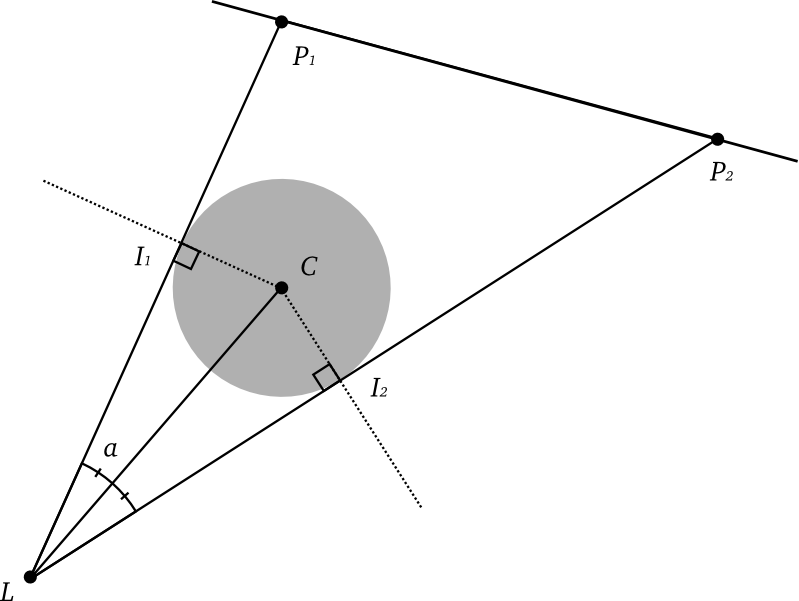
\includegraphics[width=12cm]{./figuras/ballroom.png}
\caption{Esquema del caso particular (1 columna, 1 luz, 1 pared)}
\end{figure}

Esta situaci'on se resuelve con trigonometr'ia simple: conociendo el radio de la
columna ($|I_{1}C|$) y la distancia entre la luz y el centro de la misma ($|LC|$),
podemos calcular el 'angulo $a$:

$$a = sin^{-1}\frac{|I_{1}C|}{|LC|}$$

Con el 'angulo $a$ resulta sencillo construir las intersecciones con la pared posterior.
Es importante tener en cuenta el caso en que dicha intersecci'on no existe (estamos
tratando con una semirecta de origen $L$), o se encuentra fuera del segmento que
corresponde a la pared.

Finalmente, se calcula el largo del segmento oscurecido por la columna que cae dentro
de la pared. Con este dato, el algoritmo completo es el siguiente:

\begin{algorithm}[H]
\begin{algorithmic}
\caption{Calcular la longitud del perímetro iluminado}
\FOR{cada pared}
  \FOR{cada luz}
    \FOR{cada columna}
        \STATE obtener la zona oscurecida de esta terna
    \ENDFOR
    \STATE unir todas las sombras de esta luz
    \STATE invertir las sombras para obtener las zonas iluminadas de esta luz
  \ENDFOR
  \STATE unir todas las zonas iluminadas por cada luz
  \STATE calcular la longitud iluminada en esta pared
\ENDFOR
\STATE devolver la suma de las longitudes iluminadas sobre cada pared
\end{algorithmic}
\end{algorithm}

\subsubsection{Implementaci'on}

La implementaci'on no tiene mayores particularidades. Nos encontramos con
un problema de error num'erico producto de la utilizaci�n valores obtenidos
con las funciones trigonom'etricas. Lo resolvimos utilizando \textbf{long double}
para aumentar la precisi'on de las operaciones.

Muchos de los datos utilizados en el programa son conjuntos de intervalos
que representan una porci'on (eventualmente discontinua) de los segmentos
que corresponden a las paredes. Estos conjuntos se implementaron sobre secuencias.


\subsubsection{Complejidad}

Llamaremos $C$ a la cantidad de columnas y $L$ a la cantidad de luces.

Las operaciones utilizadas por el algoritmo son:
\begin{itemize}
\item \textbf{B'usqueda de puntos de intersecci'on}, que se hace en tiempo constante en el modelo uniforme.
\item \textbf{Uni'on de conjuntos de intervalos}, que se hace en $O(n log(n))$ orden'andolos primero.
\item \textbf{Inversi'on de conjuntos de intervalos}, que se hace en $O(n)$ puesto que ya est'an ordenados.
\item \textbf{C'alculo de la longitud cubierta por el conjunto}, que se hace en $O(n)$ puesto que ya est'an ordenados.
\end{itemize}

Sabemos adem'as que cada columna tiene a lo sumo una sombra sobre cada pared. Por lo tanto,
unir todas las sombras de una luz se hace en $O(C log(C))$. En peor caso, el conjunto
resultante tiene $C$ elementos, lo que corresponde al caso en que todas las sombras
de las columnas son disjuntas.

La inversi'on se hace entonces en $O(C)$. Para los 'ultimos pasos del ciclo sobre las luces,
se unen las sombras de cada una de ellas. Dado que en peor caso tenemos $L * C$ intervalos
a unir, la uni'on resulta en un costo de $O(LC log(LC))$, seguido del c'alculo de la
longitud en tiempo lineal con un costo de $O(LC)$ dado que tras la uni'on el conjunto
de intervalos se encuentra ordenado.

Estas operaciones se hacen para cada pared, con un total de 4 que no afecta la complejidad
puesto que es constante. Finalmente, el algoritmo tiene un costo de $O(LC log(LC))$, que es
polinomial en el tama~no de la entrada puesto que la misma tiene tama\~no $O(L+C+t)$ (con
$t=log_2(max(ancho, alto))$).

\subsection{Implementaci�n}

\noindent
\ttfamily
\shorthandoff{"}\\
\hlstd{}\hlline{\ 1\ }\hldir{\#include\ $<$iostream$>$}\\
\hlline{\ 2\ }\hlstd{}\hldir{\#include\ $<$cmath$>$}\\
\hlline{\ 3\ }\hlstd{}\hldir{\#include\ $<$cstdio$>$}\\
\hlline{\ 4\ }\hlstd{}\hldir{\#include\ $<$list$>$}\\
\hlline{\ 5\ }\hlstd{}\hldir{\#include\ $<$utility$>$}\\
\hlline{\ 6\ }\hlstd{}\hldir{\#include\ $<$cstdlib$>$}\\
\hlline{\ 7\ }\hlstd{}\hldir{\#include\ $<$cassert$>$}\\
\hlline{\ 8\ }\hlstd{}\hldir{\#include\ $<$complex$>$}\\
\hlline{\ 9\ }\hlstd{}\\
\hlline{10\ }\hldir{\#define\ forn(i,\ n)\ for\ (int\ i\ =\ 0;\ i\ $<$\ (n);\ i++)}\\
\hlline{11\ }\hlstd{}\hldir{\#define\ TOLERANCIA\ 1e{-}8}\\
\hlline{12\ }\hlstd{}\\
\hlline{13\ }\hlkwa{using\ namespace\ }\hlstd{std}\hlsym{;}\\
\hlline{14\ }\hlstd{}\\
\hlline{15\ }\hlkwb{struct\ }\hlstd{MaybeDouble\ }\hlsym{\{}\\
\hlline{16\ }\hlstd{}\hlstd{\ \ \ \ }\hlstd{}\hlkwb{long\ double\ }\hlstd{valor}\hlsym{;}\\
\hlline{17\ }\hlstd{}\hlstd{\ \ \ \ }\hlstd{}\hlkwb{bool\ }\hlstd{valido}\hlsym{;}\\
\hlline{18\ }\hlstd{\\
\hlline{19\ }}\hlstd{\ \ \ \ }\hlstd{}\hlkwd{MaybeDouble}\hlstd{}\hlsym{(}\hlstd{}\hlkwb{long\ double\ }\hlstd{v}\hlsym{,\ }\hlstd{}\hlkwb{bool\ }\hlstd{b}\hlsym{):\ }\hlstd{}\hlkwd{valor}\hlstd{}\hlsym{(}\hlstd{v}\hlsym{),\ }\hlstd{}\hlkwd{valido}\hlstd{}\hlsym{(}\hlstd{b}\hlsym{)\ \{\};}\\
\hlline{20\ }\hlstd{}\hlsym{\};}\\
\hlline{21\ }\hlstd{}\\
\hlline{22\ }\hlkwb{struct\ }\hlstd{Vector\ }\hlsym{\{}\\
\hlline{23\ }\hlstd{}\hlstd{\ \ \ \ }\hlstd{}\hlkwb{long\ double\ }\hlstd{x}\hlsym{;}\\
\hlline{24\ }\hlstd{}\hlstd{\ \ \ \ }\hlstd{}\hlkwb{long\ double\ }\hlstd{y}\hlsym{;}\\
\hlline{25\ }\hlstd{\\
\hlline{26\ }}\hlstd{\ \ \ \ }\hlstd{}\hlkwd{Vector}\hlstd{}\hlsym{(}\hlstd{}\hlkwb{long\ double\ }\hlstd{xi}\hlsym{,\ }\hlstd{}\hlkwb{long\ double\ }\hlstd{yi}\hlsym{):\ }\hlstd{}\hlkwd{x}\hlstd{}\hlsym{(}\hlstd{xi}\hlsym{),\ }\hlstd{}\hlkwd{y}\hlstd{}\hlsym{(}\hlstd{yi}\hlsym{)\ \{\};}\\
\hlline{27\ }\hlstd{\\
\hlline{28\ }}\hlstd{\ \ \ \ }\hlstd{}\hlkwb{long\ double\ }\hlstd{}\hlkwd{norma}\hlstd{}\hlsym{()}\hlstd{\ \ }\hlsym{\{}\\
\hlline{29\ }\hlstd{}\hlstd{\ \ \ \ \ \ \ \ }\hlstd{}\hlkwa{return\ }\hlstd{}\hlkwd{hypot}\hlstd{}\hlsym{(}\hlstd{x}\hlsym{,\ }\hlstd{y}\hlsym{);}\\
\hlline{30\ }\hlstd{}\hlstd{\ \ \ \ }\hlstd{}\hlsym{\}}\\
\hlline{31\ }\hlstd{\\
\hlline{32\ }}\hlstd{\ \ \ \ }\hlstd{}\hlkwb{long\ double\ }\hlstd{}\hlkwd{angulo}\hlstd{}\hlsym{()\ \{}\\
\hlline{33\ }\hlstd{}\hlstd{\ \ \ \ \ \ \ \ }\hlstd{}\hlkwa{return\ }\hlstd{}\hlkwd{atan2}\hlstd{}\hlsym{(}\hlstd{y}\hlsym{,\ }\hlstd{x}\hlsym{);}\\
\hlline{34\ }\hlstd{}\hlstd{\ \ \ \ }\hlstd{}\hlsym{\}}\\
\hlline{35\ }\hlstd{}\\
\hlline{36\ }\hlsym{\};}\\
\hlline{37\ }\hlstd{}\\
\hlline{38\ }\hlkwb{struct\ }\hlstd{Columna\ }\hlsym{\{}\\
\hlline{39\ }\hlstd{}\hlstd{\ \ \ \ }\hlstd{Vector\ posicion}\hlsym{;}\\
\hlline{40\ }\hlstd{}\hlstd{\ \ \ \ }\hlstd{}\hlkwb{long\ double\ }\hlstd{radio}\hlsym{;}\\
\hlline{41\ }\hlstd{\\
\hlline{42\ }}\hlstd{\ \ \ \ }\hlstd{}\hlkwd{Columna}\hlstd{}\hlsym{(}\hlstd{}\hlkwb{long\ double\ }\hlstd{x}\hlsym{,\ }\hlstd{}\hlkwb{long\ double\ }\hlstd{y}\hlsym{,\ }\hlstd{}\hlkwb{long\ double\ }\hlstd{r}\hlsym{)\ :\ }\hlstd{}\hlkwd{posicion}\hlstd{}\hlsym{(}\hlstd{x}\hlsym{,}\hlstd{y}\hlsym{),\ }\hlstd{}\hlkwd{radio}\hlstd{}\hlsym{(}\hlstd{r}\hlsym{)\ \{\};}\\
\hlline{43\ }\hlstd{}\hlsym{\};}\\
\hlline{44\ }\hlstd{}\\
\hlline{45\ }\hlkwc{typedef\ }\hlstd{Vector\ Lampara}\hlsym{;}\\
\hlline{46\ }\hlstd{}\hlkwc{typedef\ }\hlstd{pair}\hlsym{$<$}\hlstd{}\hlkwb{long\ double}\hlstd{}\hlsym{,\ }\hlstd{}\hlkwb{long\ double}\hlstd{}\hlsym{$>$\ }\hlstd{Intervalo}\hlsym{;}\\
\hlline{47\ }\hlstd{}\hlkwc{typedef\ }\hlstd{pair}\hlsym{$<$}\hlstd{Vector}\hlsym{,\ }\hlstd{Vector}\hlsym{$>$\ }\hlstd{Segmento}\hlsym{;}\\
\hlline{48\ }\hlstd{}\\
\hlline{49\ }\\
\hlline{50\ }\hlkwc{inline\ }\hlstd{}\hlkwb{long\ double\ }\hlstd{}\hlkwd{largo}\hlstd{}\hlsym{(}\hlstd{}\hlkwb{const\ }\hlstd{Segmento}\hlsym{\&\ }\hlstd{s}\hlsym{)\ \{}\\
\hlline{51\ }\hlstd{}\hlstd{\ \ \ \ }\hlstd{}\hlkwa{return\ }\hlstd{}\hlkwd{Vector}\hlstd{}\hlsym{(}\hlstd{s}\hlsym{.}\hlstd{second}\hlsym{.}\hlstd{x\ }\hlsym{{-}\ }\hlstd{s}\hlsym{.}\hlstd{first}\hlsym{.}\hlstd{x}\hlsym{,\ }\hlstd{s}\hlsym{.}\hlstd{second}\hlsym{.}\hlstd{y\ }\hlsym{{-}\ }\hlstd{s}\hlsym{.}\hlstd{first}\hlsym{.}\hlstd{y}\hlsym{).}\hlstd{}\hlkwd{norma}\hlstd{}\hlsym{();}\\
\hlline{52\ }\hlstd{}\hlsym{\}}\\
\hlline{53\ }\hlstd{}\\
\hlline{54\ }\hlkwc{inline\ }\hlstd{}\hlkwb{long\ double\ }\hlstd{}\hlkwd{largo}\hlstd{}\hlsym{(}\hlstd{}\hlkwb{const\ }\hlstd{Intervalo}\hlsym{\&\ }\hlstd{i}\hlsym{)\ \{}\\
\hlline{55\ }\hlstd{}\hlstd{\ \ \ \ }\hlstd{}\hlkwd{assert}\hlstd{}\hlsym{(}\hlstd{i}\hlsym{.}\hlstd{first\ }\hlsym{$<$=\ }\hlstd{i}\hlsym{.}\hlstd{second}\hlsym{);}\\
\hlline{56\ }\hlstd{}\hlstd{\ \ \ \ }\hlstd{}\hlkwa{return\ }\hlstd{i}\hlsym{.}\hlstd{second\ }\hlsym{{-}\ }\hlstd{i}\hlsym{.}\hlstd{first}\hlsym{;}\\
\hlline{57\ }\hlstd{}\hlsym{\}}\\
\hlline{58\ }\hlstd{\\
\hlline{59\ }\\
\hlline{60\ }MaybeDouble\ }\hlkwd{intersect\textunderscore segments}\hlstd{}\hlsym{(}\hlstd{}\hlkwb{const\ }\hlstd{Segmento}\hlsym{\&\ }\hlstd{s1}\hlsym{,\ }\hlstd{}\hlkwb{const\ }\hlstd{Segmento}\hlsym{\&\ }\hlstd{s2}\hlsym{)\ \{}\\
\hlline{61\ }\hlstd{}\hlstd{\ \ \ \ }\hlstd{Vector\ p1\ }\hlsym{=\ }\hlstd{s1}\hlsym{.}\hlstd{first}\hlsym{;}\\
\hlline{62\ }\hlstd{}\hlstd{\ \ \ \ }\hlstd{Vector\ p2\ }\hlsym{=\ }\hlstd{s1}\hlsym{.}\hlstd{second}\hlsym{;}\\
\hlline{63\ }\hlstd{}\hlstd{\ \ \ \ }\hlstd{Vector\ p3\ }\hlsym{=\ }\hlstd{s2}\hlsym{.}\hlstd{first}\hlsym{;}\\
\hlline{64\ }\hlstd{}\hlstd{\ \ \ \ }\hlstd{Vector\ p4\ }\hlsym{=\ }\hlstd{s2}\hlsym{.}\hlstd{second}\hlsym{;}\\
\hlline{65\ }\hlstd{\\
\hlline{66\ }}\hlstd{\ \ \ \ }\hlstd{}\hlkwb{long\ double\ }\hlstd{den\ }\hlsym{=\ (}\hlstd{p4}\hlsym{.}\hlstd{y}\hlsym{{-}}\hlstd{p3}\hlsym{.}\hlstd{y}\hlsym{){*}(}\hlstd{p2}\hlsym{.}\hlstd{x}\hlsym{{-}}\hlstd{p1}\hlsym{.}\hlstd{x}\hlsym{)\ {-}\ (}\hlstd{p4}\hlsym{.}\hlstd{x}\hlsym{{-}}\hlstd{p3}\hlsym{.}\hlstd{x}\hlsym{){*}(}\hlstd{p2}\hlsym{.}\hlstd{y}\hlsym{{-}}\hlstd{p1}\hlsym{.}\hlstd{y}\hlsym{);}\\
\hlline{67\ }\hlstd{\\
\hlline{68\ }}\hlstd{\ \ \ \ }\hlstd{}\hlkwb{long\ double\ }\hlstd{ua\textunderscore num\ }\hlsym{=\ (}\hlstd{p4}\hlsym{.}\hlstd{x}\hlsym{{-}}\hlstd{p3}\hlsym{.}\hlstd{x}\hlsym{){*}(}\hlstd{p1}\hlsym{.}\hlstd{y}\hlsym{{-}}\hlstd{p3}\hlsym{.}\hlstd{y}\hlsym{)\ {-}\ (}\hlstd{p4}\hlsym{.}\hlstd{y}\hlsym{{-}}\hlstd{p3}\hlsym{.}\hlstd{y}\hlsym{){*}(}\hlstd{p1}\hlsym{.}\hlstd{x}\hlsym{{-}}\hlstd{p3}\hlsym{.}\hlstd{x}\hlsym{);}\\
\hlline{69\ }\hlstd{}\hlstd{\ \ \ \ }\hlstd{}\hlkwb{long\ double\ }\hlstd{ub\textunderscore num\ }\hlsym{=\ (}\hlstd{p2}\hlsym{.}\hlstd{x}\hlsym{{-}}\hlstd{p1}\hlsym{.}\hlstd{x}\hlsym{){*}(}\hlstd{p1}\hlsym{.}\hlstd{y}\hlsym{{-}}\hlstd{p3}\hlsym{.}\hlstd{y}\hlsym{)\ {-}\ (}\hlstd{p2}\hlsym{.}\hlstd{y}\hlsym{{-}}\hlstd{p1}\hlsym{.}\hlstd{y}\hlsym{){*}(}\hlstd{p1}\hlsym{.}\hlstd{x}\hlsym{{-}}\hlstd{p3}\hlsym{.}\hlstd{x}\hlsym{);}\\
\hlline{70\ }\hlstd{\\
\hlline{71\ }}\hlstd{\ \ \ \ }\hlstd{}\hlkwa{if\ }\hlstd{}\hlsym{(}\hlstd{}\hlkwd{fabs}\hlstd{}\hlsym{(}\hlstd{den}\hlsym{)\ $<$\ }\hlstd{TOLERANCIA}\hlsym{)\ \{}\\
\hlline{72\ }\hlstd{}\hlstd{\ \ \ \ \ \ \ \ }\hlstd{}\hlslc{//\ Caso\ en\ que\ los\ segmentos\ son\ paralelos}\\
\hlline{73\ }\hlstd{}\hlstd{\ \ \ \ \ \ \ \ }\hlstd{}\hlkwa{if\ }\hlstd{}\hlsym{(}\hlstd{}\hlkwd{fabs}\hlstd{}\hlsym{(}\hlstd{ua\textunderscore num\ }\hlsym{{-}\ }\hlstd{ub\textunderscore num}\hlsym{)\ $<$\ }\hlstd{TOLERANCIA\ }\hlsym{\&\&\ }\hlstd{}\hlkwd{fabs}\hlstd{}\hlsym{(}\hlstd{ub\textunderscore num}\hlsym{)\ $<$\ }\hlstd{TOLERANCIA}\hlsym{)\ \{}\\
\hlline{74\ }\hlstd{}\hlstd{\ \ \ \ \ \ \ \ \ \ \ \ }\hlstd{}\hlslc{//\ Las\ rectas\ son\ coincidentes,\ esto\ no\ deberia\ ocurrir}\\
\hlline{75\ }\hlstd{}\hlstd{\ \ \ \ \ \ \ \ \ \ \ \ }\hlstd{}\hlkwd{assert}\hlstd{}\hlsym{(}\hlstd{}\hlkwa{false}\hlstd{}\hlsym{);}\\
\hlline{76\ }\hlstd{}\hlstd{\ \ \ \ \ \ \ \ \ \ \ \ }\hlstd{}\hlkwa{return\ }\hlstd{}\hlkwd{MaybeDouble}\hlstd{}\hlsym{((}\hlstd{p1}\hlsym{.}\hlstd{}\hlkwd{norma}\hlstd{}\hlsym{()\ $>$\ }\hlstd{p2}\hlsym{.}\hlstd{}\hlkwd{norma}\hlstd{}\hlsym{()}\hlstd{?\ }\hlnum{0\ }\hlstd{}\hlsym{:\ }\hlstd{}\hlnum{1}\hlstd{}\hlsym{),\ }\hlstd{}\hlkwa{true}\hlstd{}\hlsym{);}\\
\hlline{77\ }\hlstd{}\hlstd{\ \ \ \ \ \ \ \ }\hlstd{}\hlsym{\}}\\
\hlline{78\ }\hlstd{}\hlstd{\ \ \ \ \ \ \ \ }\hlstd{}\hlkwa{return\ }\hlstd{}\hlkwd{MaybeDouble}\hlstd{}\hlsym{(}\hlstd{}\hlnum{0}\hlstd{}\hlsym{,\ }\hlstd{}\hlkwa{false}\hlstd{}\hlsym{);}\\
\hlline{79\ }\hlstd{}\hlstd{\ \ \ \ }\hlstd{}\hlsym{\}}\\
\hlline{80\ }\hlstd{\\
\hlline{81\ }}\hlstd{\ \ \ \ }\hlstd{}\hlkwa{if\ }\hlstd{}\hlsym{(}\hlstd{ub\textunderscore num}\hlsym{/}\hlstd{den\ }\hlsym{$>$=\ }\hlstd{}\hlnum{0}\hlstd{}\hlsym{)\ \{}\\
\hlline{82\ }\hlstd{}\hlstd{\ \ \ \ \ \ \ \ }\hlstd{}\hlkwa{return\ }\hlstd{}\hlkwd{MaybeDouble}\hlstd{}\hlsym{(}\hlstd{ua\textunderscore num}\hlsym{/}\hlstd{den}\hlsym{,\ }\hlstd{}\hlkwa{true}\hlstd{}\hlsym{);}\\
\hlline{83\ }\hlstd{}\hlstd{\ \ \ \ }\hlstd{}\hlsym{\}}\\
\hlline{84\ }\hlstd{}\hlstd{\ \ \ \ }\hlstd{}\hlkwa{return\ }\hlstd{}\hlkwd{MaybeDouble}\hlstd{}\hlsym{(}\hlstd{}\hlnum{0}\hlstd{}\hlsym{,\ }\hlstd{}\hlkwa{false}\hlstd{}\hlsym{);}\\
\hlline{85\ }\hlstd{}\hlsym{\}}\\
\hlline{86\ }\hlstd{\\
\hlline{87\ }\\
\hlline{88\ }Intervalo\ }\hlkwd{interseccion\textunderscore intervalos}\hlstd{}\hlsym{(}\hlstd{}\hlkwb{const\ }\hlstd{Intervalo}\hlsym{\&\ }\hlstd{i1}\hlsym{,\ }\hlstd{}\hlkwb{const\ }\hlstd{Intervalo}\hlsym{\&\ }\hlstd{i2}\hlsym{)\ \{}\\
\hlline{89\ }\hlstd{\\
\hlline{90\ }}\hlstd{\ \ \ \ }\hlstd{}\hlkwb{long\ double\ }\hlstd{d0\ }\hlsym{=\ }\hlstd{}\hlkwd{max}\hlstd{}\hlsym{(}\hlstd{i1}\hlsym{.}\hlstd{first}\hlsym{,\ }\hlstd{i2}\hlsym{.}\hlstd{first}\hlsym{);}\\
\hlline{91\ }\hlstd{}\hlstd{\ \ \ \ }\hlstd{}\hlkwb{long\ double\ }\hlstd{d1\ }\hlsym{=\ }\hlstd{}\hlkwd{min}\hlstd{}\hlsym{(}\hlstd{i1}\hlsym{.}\hlstd{second}\hlsym{,\ }\hlstd{i2}\hlsym{.}\hlstd{second}\hlsym{);}\\
\hlline{92\ }\hlstd{\\
\hlline{93\ }}\hlstd{\ \ \ \ }\hlstd{}\hlkwa{if\ }\hlstd{}\hlsym{(}\hlstd{d1\ }\hlsym{$<$\ }\hlstd{d0}\hlsym{)\ \{}\\
\hlline{94\ }\hlstd{}\hlstd{\ \ \ \ \ \ \ \ }\hlstd{}\hlkwa{return\ }\hlstd{}\hlkwd{Intervalo}\hlstd{}\hlsym{(}\hlstd{}\hlnum{0}\hlstd{}\hlsym{,\ }\hlstd{}\hlnum{0}\hlstd{}\hlsym{);}\\
\hlline{95\ }\hlstd{}\hlstd{\ \ \ \ }\hlstd{}\hlsym{\}\ }\hlstd{}\hlkwa{else\ }\hlstd{}\hlsym{\{}\\
\hlline{96\ }\hlstd{}\hlstd{\ \ \ \ \ \ \ \ }\hlstd{}\hlkwa{return\ }\hlstd{}\hlkwd{Intervalo}\hlstd{}\hlsym{(}\hlstd{d0}\hlsym{,\ }\hlstd{d1}\hlsym{);}\\
\hlline{97\ }\hlstd{}\hlstd{\ \ \ \ }\hlstd{}\hlsym{\}}\\
\hlline{98\ }\hlstd{}\hlsym{\}}\\
\hlline{99\ }\hlstd{\\
\hlline{100\ }\\
\hlline{101\ }Intervalo\ }\hlkwd{rango\textunderscore oscurecido}\hlstd{}\hlsym{(}\hlstd{}\hlkwb{const\ }\hlstd{Segmento}\hlsym{\&\ }\hlstd{pared}\hlsym{,\ }\hlstd{}\hlkwb{const\ }\hlstd{Lampara}\hlsym{\&\ }\hlstd{lampara}\hlsym{,\ }\hlstd{}\hlkwb{const\ }\hlstd{Columna}\hlsym{\&\ }\hlstd{columna}\hlsym{)\ \{}\\
\hlline{102\ }\hlstd{}\hlstd{\ \ \ \ }\hlstd{Vector\ }\hlkwd{bisectriz}\hlstd{}\hlsym{(}\hlstd{columna}\hlsym{.}\hlstd{posicion}\hlsym{.}\hlstd{x\ }\hlsym{{-}\ }\hlstd{lampara}\hlsym{.}\hlstd{x}\hlsym{,\ }\hlstd{columna}\hlsym{.}\hlstd{posicion}\hlsym{.}\hlstd{y\ }\hlsym{{-}\ }\hlstd{lampara}\hlsym{.}\hlstd{y}\hlsym{);}\\
\hlline{103\ }\hlstd{}\hlstd{\ \ \ \ }\hlstd{}\hlkwb{long\ double\ }\hlstd{p\ }\hlsym{=\ }\hlstd{}\hlkwd{asin}\hlstd{}\hlsym{(}\hlstd{columna}\hlsym{.}\hlstd{radio}\hlsym{/}\hlstd{bisectriz}\hlsym{.}\hlstd{}\hlkwd{norma}\hlstd{}\hlsym{());}\\
\hlline{104\ }\hlstd{}\hlstd{\ \ \ \ }\hlstd{}\hlkwb{long\ double\ }\hlstd{alpha\ }\hlsym{=\ }\hlstd{bisectriz}\hlsym{.}\hlstd{}\hlkwd{angulo}\hlstd{}\hlsym{();}\\
\hlline{105\ }\hlstd{\\
\hlline{106\ }}\hlstd{\ \ \ \ }\hlstd{Vector\ }\hlkwd{d1}\hlstd{}\hlsym{(}\hlstd{}\hlkwd{cos}\hlstd{}\hlsym{(}\hlstd{alpha\ }\hlsym{+\ }\hlstd{p}\hlsym{),\ }\hlstd{}\hlkwd{sin}\hlstd{}\hlsym{(}\hlstd{alpha\ }\hlsym{+\ }\hlstd{p}\hlsym{));}\\
\hlline{107\ }\hlstd{}\hlstd{\ \ \ \ }\hlstd{Vector\ }\hlkwd{d2}\hlstd{}\hlsym{(}\hlstd{}\hlkwd{cos}\hlstd{}\hlsym{(}\hlstd{alpha\ }\hlsym{{-}\ }\hlstd{p}\hlsym{),\ }\hlstd{}\hlkwd{sin}\hlstd{}\hlsym{(}\hlstd{alpha\ }\hlsym{{-}\ }\hlstd{p}\hlsym{));}\\
\hlline{108\ }\hlstd{\\
\hlline{109\ }}\hlstd{\ \ \ \ }\hlstd{MaybeDouble\ p1\ }\hlsym{=\ }\hlstd{}\hlkwd{intersect\textunderscore segments}\hlstd{}\hlsym{(}\hlstd{pared}\hlsym{,\ }\hlstd{}\hlkwd{Segmento}\hlstd{}\hlsym{(}\hlstd{lampara}\hlsym{,\ }\hlstd{}\hlkwd{Vector}\hlstd{}\hlsym{(}\hlstd{lampara}\hlsym{.}\hlstd{x\ }\hlsym{+\ }\hlstd{d1}\hlsym{.}\hlstd{x}\hlsym{,\ }\hlstd{lampara}\hlsym{.}\hlstd{y\ }\hlsym{+}\Righttorque\\
\hlline{110\ }\hlstd{}\hlstd{\ \ \ \ \ \ \ \ \ \ \ \ \ \ \ \ \ \ \ \ \ }\hlstd{d1}\hlsym{.}\hlstd{y}\hlsym{)));}\\
\hlline{111\ }\hlstd{}\hlstd{\ \ \ \ }\hlstd{MaybeDouble\ p2\ }\hlsym{=\ }\hlstd{}\hlkwd{intersect\textunderscore segments}\hlstd{}\hlsym{(}\hlstd{pared}\hlsym{,\ }\hlstd{}\hlkwd{Segmento}\hlstd{}\hlsym{(}\hlstd{lampara}\hlsym{,\ }\hlstd{}\hlkwd{Vector}\hlstd{}\hlsym{(}\hlstd{lampara}\hlsym{.}\hlstd{x\ }\hlsym{+\ }\hlstd{d2}\hlsym{.}\hlstd{x}\hlsym{,\ }\hlstd{lampara}\hlsym{.}\hlstd{y\ }\hlsym{+}\Righttorque\\
\hlline{112\ }\hlstd{}\hlstd{\ \ \ \ \ \ \ \ \ \ \ \ \ \ \ \ \ \ \ \ \ }\hlstd{d2}\hlsym{.}\hlstd{y}\hlsym{)));}\\
\hlline{113\ }\hlstd{\\
\hlline{114\ }}\hlstd{\ \ \ \ }\hlstd{}\hlkwb{long\ double\ }\hlstd{unidad\ }\hlsym{=\ }\hlstd{}\hlkwd{largo}\hlstd{}\hlsym{(}\hlstd{pared}\hlsym{);}\\
\hlline{115\ }\hlstd{\\
\hlline{116\ }}\hlstd{\ \ \ \ }\hlstd{}\hlslc{//\ Se\ sabe\ que\ los\ puntos\ de\ interseccion\ estan\ ordenados\ correctamente}\\
\hlline{117\ }\hlstd{}\hlstd{\ \ \ \ }\hlstd{}\hlslc{//\ porque\ el\ angulo\ de\ diferencia\ entre\ las\ semirectas\ es\ menor\ a\ 180,}\\
\hlline{118\ }\hlstd{}\hlstd{\ \ \ \ }\hlstd{}\hlslc{//\ entonces\ no\ es\ necesario\ chequearlo.}\\
\hlline{119\ }\hlstd{}\hlstd{\ \ \ \ }\hlstd{Intervalo\ res}\hlsym{;}\\
\hlline{120\ }\hlstd{\\
\hlline{121\ }}\hlstd{\ \ \ \ }\hlstd{}\hlkwa{if\ }\hlstd{}\hlsym{(!}\hlstd{p1}\hlsym{.}\hlstd{valido}\hlsym{)\ \{}\\
\hlline{122\ }\hlstd{}\hlstd{\ \ \ \ \ \ \ \ }\hlstd{}\hlkwa{if\ }\hlstd{}\hlsym{(!}\hlstd{p2}\hlsym{.}\hlstd{valido}\hlsym{)\ \{}\\
\hlline{123\ }\hlstd{}\hlstd{\ \ \ \ \ \ \ \ \ \ \ \ }\hlstd{}\hlkwa{return\ }\hlstd{}\hlkwd{Intervalo}\hlstd{}\hlsym{(}\hlstd{}\hlnum{0}\hlstd{}\hlsym{,\ }\hlstd{}\hlnum{0}\hlstd{}\hlsym{);}\\
\hlline{124\ }\hlstd{}\hlstd{\ \ \ \ \ \ \ \ }\hlstd{}\hlsym{\}\ }\hlstd{}\hlkwa{else\ }\hlstd{}\hlsym{\{}\\
\hlline{125\ }\hlstd{}\hlstd{\ \ \ \ \ \ \ \ \ \ \ \ }\hlstd{res\ }\hlsym{=\ }\hlstd{}\hlkwd{Intervalo}\hlstd{}\hlsym{(}\hlstd{}\hlnum{0}\hlstd{}\hlsym{,\ }\hlstd{p2}\hlsym{.}\hlstd{valor}\hlsym{);}\\
\hlline{126\ }\hlstd{}\hlstd{\ \ \ \ \ \ \ \ }\hlstd{}\hlsym{\}}\\
\hlline{127\ }\hlstd{}\hlstd{\ \ \ \ }\hlstd{}\hlsym{\}\ }\hlstd{}\hlkwa{else\ }\hlstd{}\hlsym{\{}\\
\hlline{128\ }\hlstd{}\hlstd{\ \ \ \ \ \ \ \ }\hlstd{}\hlkwa{if\ }\hlstd{}\hlsym{(!}\hlstd{p2}\hlsym{.}\hlstd{valido}\hlsym{)\ \{}\\
\hlline{129\ }\hlstd{}\hlstd{\ \ \ \ \ \ \ \ \ \ \ \ }\hlstd{res\ }\hlsym{=\ }\hlstd{}\hlkwd{Intervalo}\hlstd{}\hlsym{(}\hlstd{p1}\hlsym{.}\hlstd{valor}\hlsym{,\ }\hlstd{}\hlnum{1}\hlstd{}\hlsym{);}\\
\hlline{130\ }\hlstd{}\hlstd{\ \ \ \ \ \ \ \ }\hlstd{}\hlsym{\}\ }\hlstd{}\hlkwa{else\ }\hlstd{}\hlsym{\{}\\
\hlline{131\ }\hlstd{}\hlstd{\ \ \ \ \ \ \ \ \ \ \ \ }\hlstd{res\ }\hlsym{=\ }\hlstd{}\hlkwd{Intervalo}\hlstd{}\hlsym{(}\hlstd{p1}\hlsym{.}\hlstd{valor}\hlsym{,\ }\hlstd{p2}\hlsym{.}\hlstd{valor}\hlsym{);}\\
\hlline{132\ }\hlstd{}\hlstd{\ \ \ \ \ \ \ \ }\hlstd{}\hlsym{\}}\\
\hlline{133\ }\hlstd{}\hlstd{\ \ \ \ }\hlstd{}\hlsym{\}}\\
\hlline{134\ }\hlstd{\\
\hlline{135\ }}\hlstd{\ \ \ \ }\hlstd{res\ }\hlsym{=\ }\hlstd{}\hlkwd{interseccion\textunderscore intervalos}\hlstd{}\hlsym{(}\hlstd{res}\hlsym{,\ }\hlstd{}\hlkwd{Intervalo}\hlstd{}\hlsym{(}\hlstd{}\hlnum{0}\hlstd{}\hlsym{,}\hlstd{}\hlnum{1}\hlstd{}\hlsym{));}\\
\hlline{136\ }\hlstd{}\hlstd{\ \ \ \ }\hlstd{}\hlkwa{return\ }\hlstd{}\hlkwd{Intervalo}\hlstd{}\hlsym{(}\hlstd{res}\hlsym{.}\hlstd{first\ }\hlsym{{*}\ }\hlstd{unidad}\hlsym{,\ }\hlstd{res}\hlsym{.}\hlstd{second\ }\hlsym{{*}\ }\hlstd{unidad}\hlsym{);}\\
\hlline{137\ }\hlstd{}\hlsym{\}}\\
\hlline{138\ }\hlstd{}\\
\hlline{139\ }\hlkwb{void\ }\hlstd{}\hlkwd{invertir\textunderscore rango}\hlstd{}\hlsym{(}\hlstd{}\hlkwb{const\ }\hlstd{list}\hlsym{$<$}\hlstd{Intervalo}\hlsym{$>$\&\ }\hlstd{ints}\hlsym{,\ }\hlstd{}\hlkwb{long\ double\ }\hlstd{fin}\hlsym{,\ }\hlstd{list}\hlsym{$<$}\hlstd{Intervalo}\hlsym{$>$\&\ }\hlstd{out}\hlsym{)\ \{}\\
\hlline{140\ }\hlstd{\\
\hlline{141\ }}\hlstd{\ \ \ \ }\hlstd{}\hlkwa{if\ }\hlstd{}\hlsym{(!}\hlstd{ints}\hlsym{.}\hlstd{}\hlkwd{size}\hlstd{}\hlsym{())\ \{}\\
\hlline{142\ }\hlstd{}\hlstd{\ \ \ \ \ \ \ \ }\hlstd{out}\hlsym{.}\hlstd{}\hlkwd{push\textunderscore back}\hlstd{}\hlsym{(}\hlstd{}\hlkwd{Intervalo}\hlstd{}\hlsym{(}\hlstd{}\hlnum{0}\hlstd{}\hlsym{,}\hlstd{fin}\hlsym{));}\\
\hlline{143\ }\hlstd{}\hlstd{\ \ \ \ \ \ \ \ }\hlstd{}\hlkwa{return}\hlstd{}\hlsym{;}\\
\hlline{144\ }\hlstd{}\hlstd{\ \ \ \ }\hlstd{}\hlsym{\}}\\
\hlline{145\ }\hlstd{\\
\hlline{146\ }\\
\hlline{147\ }}\hlstd{\ \ \ \ }\hlstd{list}\hlsym{$<$}\hlstd{Intervalo}\hlsym{$>$::}\hlstd{const\textunderscore iterator\ it\ }\hlsym{=\ }\hlstd{ints}\hlsym{.}\hlstd{}\hlkwd{begin}\hlstd{}\hlsym{();}\\
\hlline{148\ }\hlstd{}\hlstd{\ \ \ \ }\hlstd{}\hlkwa{if\ }\hlstd{}\hlsym{(}\hlstd{it}\hlsym{{-}$>$}\hlstd{first\ }\hlsym{$>$\ }\hlstd{}\hlnum{0}\hlstd{}\hlsym{)\ \{}\\
\hlline{149\ }\hlstd{}\hlstd{\ \ \ \ \ \ \ \ }\hlstd{out}\hlsym{.}\hlstd{}\hlkwd{push\textunderscore back}\hlstd{}\hlsym{(}\hlstd{}\hlkwd{Intervalo}\hlstd{}\hlsym{(}\hlstd{}\hlnum{0}\hlstd{}\hlsym{,\ }\hlstd{it}\hlsym{{-}$>$}\hlstd{first}\hlsym{));}\\
\hlline{150\ }\hlstd{}\hlstd{\ \ \ \ }\hlstd{}\hlsym{\}}\\
\hlline{151\ }\hlstd{\\
\hlline{152\ }}\hlstd{\ \ \ \ }\hlstd{it}\hlsym{++;}\\
\hlline{153\ }\hlstd{\\
\hlline{154\ }}\hlstd{\ \ \ \ }\hlstd{list}\hlsym{$<$}\hlstd{Intervalo}\hlsym{$>$::}\hlstd{const\textunderscore iterator\ itprev\ }\hlsym{=\ }\hlstd{ints}\hlsym{.}\hlstd{}\hlkwd{begin}\hlstd{}\hlsym{();}\\
\hlline{155\ }\hlstd{}\hlstd{\ \ \ \ }\hlstd{}\hlkwa{while\ }\hlstd{}\hlsym{(}\hlstd{it\ }\hlsym{!=\ }\hlstd{ints}\hlsym{.}\hlstd{}\hlkwd{end}\hlstd{}\hlsym{())\ \{}\\
\hlline{156\ }\hlstd{}\hlstd{\ \ \ \ \ \ \ \ }\hlstd{out}\hlsym{.}\hlstd{}\hlkwd{push\textunderscore back}\hlstd{}\hlsym{(}\hlstd{}\hlkwd{Intervalo}\hlstd{}\hlsym{(}\hlstd{itprev}\hlsym{{-}$>$}\hlstd{second}\hlsym{,\ }\hlstd{it}\hlsym{{-}$>$}\hlstd{first}\hlsym{));}\\
\hlline{157\ }\hlstd{}\hlstd{\ \ \ \ \ \ \ \ }\hlstd{it}\hlsym{++;}\\
\hlline{158\ }\hlstd{}\hlstd{\ \ \ \ \ \ \ \ }\hlstd{itprev}\hlsym{++;}\\
\hlline{159\ }\hlstd{}\hlstd{\ \ \ \ }\hlstd{}\hlsym{\}}\\
\hlline{160\ }\hlstd{\\
\hlline{161\ }}\hlstd{\ \ \ \ }\hlstd{}\hlkwa{if\ }\hlstd{}\hlsym{(}\hlstd{itprev}\hlsym{{-}$>$}\hlstd{second\ }\hlsym{$<$\ }\hlstd{fin}\hlsym{)\ \{}\\
\hlline{162\ }\hlstd{}\hlstd{\ \ \ \ \ \ \ \ }\hlstd{out}\hlsym{.}\hlstd{}\hlkwd{push\textunderscore back}\hlstd{}\hlsym{(}\hlstd{}\hlkwd{Intervalo}\hlstd{}\hlsym{(}\hlstd{itprev}\hlsym{{-}$>$}\hlstd{second}\hlsym{,\ }\hlstd{fin}\hlsym{));}\\
\hlline{163\ }\hlstd{}\hlstd{\ \ \ \ }\hlstd{}\hlsym{\}}\\
\hlline{164\ }\hlstd{}\hlsym{\}}\\
\hlline{165\ }\hlstd{}\\
\hlline{166\ }\\
\hlline{167\ }\hlkwb{void\ }\hlstd{}\hlkwd{reduce\textunderscore union}\hlstd{}\hlsym{(}\hlstd{list}\hlsym{$<$}\hlstd{Intervalo}\hlsym{$>$\&\ }\hlstd{l\textunderscore o}\hlsym{,\ }\hlstd{list}\hlsym{$<$}\hlstd{Intervalo}\hlsym{$>$\&\ }\hlstd{out}\hlsym{)\ \{}\\
\hlline{168\ }\hlstd{}\hlstd{\ \ \ \ }\hlstd{}\hlslc{//\ elimino\ repetidos\ para\ acelerar\ el\ sort}\\
\hlline{169\ }\hlstd{}\hlstd{\ \ \ \ }\hlstd{list}\hlsym{$<$}\hlstd{Intervalo}\hlsym{$>$\ }\hlstd{l}\hlsym{;}\\
\hlline{170\ }\hlstd{\\
\hlline{171\ }}\hlstd{\ \ \ \ }\hlstd{}\hlkwa{for\ }\hlstd{}\hlsym{(}\hlstd{list}\hlsym{$<$}\hlstd{Intervalo}\hlsym{$>$::}\hlstd{const\textunderscore iterator\ itcito\ }\hlsym{=\ }\hlstd{l\textunderscore o}\hlsym{.}\hlstd{}\hlkwd{begin}\hlstd{}\hlsym{();\ }\hlstd{itcito\ }\hlsym{!=\ }\hlstd{l\textunderscore o}\hlsym{.}\hlstd{}\hlkwd{end}\hlstd{}\hlsym{();\ }\hlstd{itcito}\hlsym{++)\ \{}\\
\hlline{172\ }\hlstd{}\hlstd{\ \ \ \ \ \ \ \ }\hlstd{}\hlkwa{if\ }\hlstd{}\hlsym{(}\hlstd{itcito}\hlsym{{-}$>$}\hlstd{first\ }\hlsym{$<$\ }\hlstd{itcito}\hlsym{{-}$>$}\hlstd{second}\hlsym{)\ \{}\\
\hlline{173\ }\hlstd{}\hlstd{\ \ \ \ \ \ \ \ \ \ \ \ }\hlstd{l}\hlsym{.}\hlstd{}\hlkwd{push\textunderscore back}\hlstd{}\hlsym{(}\hlstd{}\hlkwd{Intervalo}\hlstd{}\hlsym{(}\hlstd{itcito}\hlsym{{-}$>$}\hlstd{first}\hlsym{,\ }\hlstd{itcito}\hlsym{{-}$>$}\hlstd{second}\hlsym{));}\\
\hlline{174\ }\hlstd{}\hlstd{\ \ \ \ \ \ \ \ }\hlstd{}\hlsym{\}\ }\hlstd{}\hlkwa{else\ if\ }\hlstd{}\hlsym{(}\hlstd{itcito}\hlsym{{-}$>$}\hlstd{first\ }\hlsym{$>$\ }\hlstd{itcito}\hlsym{{-}$>$}\hlstd{second}\hlsym{)\ \{}\\
\hlline{175\ }\hlstd{}\hlstd{\ \ \ \ \ \ \ \ \ \ \ \ }\hlstd{}\hlkwd{assert}\hlstd{}\hlsym{(}\hlstd{}\hlkwa{false}\hlstd{}\hlsym{);}\\
\hlline{176\ }\hlstd{}\hlstd{\ \ \ \ \ \ \ \ }\hlstd{}\hlsym{\}}\\
\hlline{177\ }\hlstd{}\hlstd{\ \ \ \ }\hlstd{}\hlsym{\}}\\
\hlline{178\ }\hlstd{\\
\hlline{179\ }\\
\hlline{180\ }}\hlstd{\ \ \ \ }\hlstd{}\hlkwa{if\ }\hlstd{}\hlsym{(!}\hlstd{l}\hlsym{.}\hlstd{}\hlkwd{size}\hlstd{}\hlsym{())\ }\hlstd{}\hlkwa{return}\hlstd{}\hlsym{;}\\
\hlline{181\ }\hlstd{\\
\hlline{182\ }}\hlstd{\ \ \ \ }\hlstd{l}\hlsym{.}\hlstd{}\hlkwd{sort}\hlstd{}\hlsym{();}\\
\hlline{183\ }\hlstd{\\
\hlline{184\ }}\hlstd{\ \ \ \ }\hlstd{list}\hlsym{$<$}\hlstd{Intervalo}\hlsym{$>$::}\hlstd{const\textunderscore iterator\ it\ }\hlsym{=\ }\hlstd{l}\hlsym{.}\hlstd{}\hlkwd{begin}\hlstd{}\hlsym{();}\\
\hlline{185\ }\hlstd{}\hlstd{\ \ \ \ }\hlstd{Intervalo\ cand\ }\hlsym{=\ {*}}\hlstd{it}\hlsym{;}\\
\hlline{186\ }\hlstd{}\hlstd{\ \ \ \ }\hlstd{Intervalo\ otro}\hlsym{;}\\
\hlline{187\ }\hlstd{\\
\hlline{188\ }}\hlstd{\ \ \ \ }\hlstd{it}\hlsym{++;}\\
\hlline{189\ }\hlstd{}\hlstd{\ \ \ \ }\hlstd{}\hlkwa{while\ }\hlstd{}\hlsym{(}\hlstd{it\ }\hlsym{!=\ }\hlstd{l}\hlsym{.}\hlstd{}\hlkwd{end}\hlstd{}\hlsym{())\ \{}\\
\hlline{190\ }\hlstd{}\hlstd{\ \ \ \ \ \ \ \ }\hlstd{otro\ }\hlsym{=\ {*}}\hlstd{it}\hlsym{;}\\
\hlline{191\ }\hlstd{}\hlstd{\ \ \ \ \ \ \ \ }\hlstd{}\hlkwa{if\ }\hlstd{}\hlsym{(}\hlstd{otro}\hlsym{.}\hlstd{first\ }\hlsym{$<$\ }\hlstd{otro}\hlsym{.}\hlstd{second}\hlsym{)\ \{}\\
\hlline{192\ }\hlstd{}\hlstd{\ \ \ \ \ \ \ \ \ \ \ \ }\hlstd{}\hlkwa{if\ }\hlstd{}\hlsym{(}\hlstd{otro}\hlsym{.}\hlstd{first\ }\hlsym{$>$\ }\hlstd{cand}\hlsym{.}\hlstd{second}\hlsym{)\ \{}\\
\hlline{193\ }\hlstd{}\hlstd{\ \ \ \ \ \ \ \ \ \ \ \ \ \ \ \ }\hlstd{out}\hlsym{.}\hlstd{}\hlkwd{push\textunderscore back}\hlstd{}\hlsym{(}\hlstd{cand}\hlsym{);}\\
\hlline{194\ }\hlstd{}\hlstd{\ \ \ \ \ \ \ \ \ \ \ \ \ \ \ \ }\hlstd{cand\ }\hlsym{=\ }\hlstd{otro}\hlsym{;}\\
\hlline{195\ }\hlstd{}\hlstd{\ \ \ \ \ \ \ \ \ \ \ \ }\hlstd{}\hlsym{\}\ }\hlstd{}\hlkwa{else\ }\hlstd{}\hlsym{\{}\\
\hlline{196\ }\hlstd{}\hlstd{\ \ \ \ \ \ \ \ \ \ \ \ \ \ \ \ }\hlstd{}\hlkwa{if\ }\hlstd{}\hlsym{(}\hlstd{otro}\hlsym{.}\hlstd{second\ }\hlsym{$>$\ }\hlstd{cand}\hlsym{.}\hlstd{second}\hlsym{)\ \{}\\
\hlline{197\ }\hlstd{}\hlstd{\ \ \ \ \ \ \ \ \ \ \ \ \ \ \ \ \ \ \ \ }\hlstd{cand\ }\hlsym{=\ }\hlstd{}\hlkwd{Intervalo}\hlstd{}\hlsym{(}\hlstd{cand}\hlsym{.}\hlstd{first}\hlsym{,\ }\hlstd{otro}\hlsym{.}\hlstd{second}\hlsym{);}\\
\hlline{198\ }\hlstd{}\hlstd{\ \ \ \ \ \ \ \ \ \ \ \ \ \ \ \ }\hlstd{}\hlsym{\}}\\
\hlline{199\ }\hlstd{}\hlstd{\ \ \ \ \ \ \ \ \ \ \ \ }\hlstd{}\hlsym{\}}\\
\hlline{200\ }\hlstd{}\hlstd{\ \ \ \ \ \ \ \ }\hlstd{}\hlsym{\}}\\
\hlline{201\ }\hlstd{}\hlstd{\ \ \ \ \ \ \ \ }\hlstd{it}\hlsym{++;}\\
\hlline{202\ }\hlstd{}\hlstd{\ \ \ \ }\hlstd{}\hlsym{\}}\\
\hlline{203\ }\hlstd{\\
\hlline{204\ }}\hlstd{\ \ \ \ }\hlstd{out}\hlsym{.}\hlstd{}\hlkwd{push\textunderscore back}\hlstd{}\hlsym{(}\hlstd{cand}\hlsym{);}\\
\hlline{205\ }\hlstd{}\hlsym{\}}\\
\hlline{206\ }\hlstd{}\\
\hlline{207\ }\\
\hlline{208\ }\hlkwb{long\ double\ }\hlstd{}\hlkwd{resolver}\hlstd{}\hlsym{(}\hlstd{}\hlkwb{const\ }\hlstd{list}\hlsym{$<$}\hlstd{Lampara}\hlsym{$>$\&\ }\hlstd{lamparas}\hlsym{,\ }\hlstd{}\hlkwb{const\ }\hlstd{list}\hlsym{$<$}\hlstd{Columna}\hlsym{$>$\&\ }\hlstd{columnas}\hlsym{,\ }\hlstd{}\hlkwb{int\ }\hlstd{max\textunderscore x}\hlsym{,\ }\hlstd{}\hlkwb{int\ }\Righttorque\\
\hlline{209\ }\hlstd{}\hlstd{\ \ \ \ \ \ \ \ \ \ \ \ \ \ \ \ \ \ \ \ \ }\hlstd{max\textunderscore y}\hlsym{)\ \{}\\
\hlline{210\ }\hlstd{}\hlstd{\ \ \ \ }\hlstd{list}\hlsym{$<$}\hlstd{Segmento}\hlsym{$>$\ }\hlstd{paredes}\hlsym{;}\\
\hlline{211\ }\hlstd{}\hlstd{\ \ \ \ }\hlstd{paredes}\hlsym{.}\hlstd{}\hlkwd{push\textunderscore back}\hlstd{}\hlsym{(}\hlstd{}\hlkwd{Segmento}\hlstd{}\hlsym{(}\hlstd{}\hlkwd{Vector}\hlstd{}\hlsym{(}\hlstd{}\hlnum{0}\hlstd{}\hlsym{,}\hlstd{}\hlnum{0}\hlstd{}\hlsym{),\ }\hlstd{}\hlkwd{Vector}\hlstd{}\hlsym{(}\hlstd{}\hlnum{0}\hlstd{}\hlsym{,\ }\hlstd{max\textunderscore y}\hlsym{)));}\\
\hlline{212\ }\hlstd{}\hlstd{\ \ \ \ }\hlstd{paredes}\hlsym{.}\hlstd{}\hlkwd{push\textunderscore back}\hlstd{}\hlsym{(}\hlstd{}\hlkwd{Segmento}\hlstd{}\hlsym{(}\hlstd{}\hlkwd{Vector}\hlstd{}\hlsym{(}\hlstd{}\hlnum{0}\hlstd{}\hlsym{,}\hlstd{max\textunderscore y}\hlsym{),\ }\hlstd{}\hlkwd{Vector}\hlstd{}\hlsym{(}\hlstd{max\textunderscore x}\hlsym{,\ }\hlstd{max\textunderscore y}\hlsym{)));}\\
\hlline{213\ }\hlstd{}\hlstd{\ \ \ \ }\hlstd{paredes}\hlsym{.}\hlstd{}\hlkwd{push\textunderscore back}\hlstd{}\hlsym{(}\hlstd{}\hlkwd{Segmento}\hlstd{}\hlsym{(}\hlstd{}\hlkwd{Vector}\hlstd{}\hlsym{(}\hlstd{max\textunderscore x}\hlsym{,}\hlstd{max\textunderscore y}\hlsym{),\ }\hlstd{}\hlkwd{Vector}\hlstd{}\hlsym{(}\hlstd{max\textunderscore x}\hlsym{,\ }\hlstd{}\hlnum{0}\hlstd{}\hlsym{)));}\\
\hlline{214\ }\hlstd{}\hlstd{\ \ \ \ }\hlstd{paredes}\hlsym{.}\hlstd{}\hlkwd{push\textunderscore back}\hlstd{}\hlsym{(}\hlstd{}\hlkwd{Segmento}\hlstd{}\hlsym{(}\hlstd{}\hlkwd{Vector}\hlstd{}\hlsym{(}\hlstd{max\textunderscore x}\hlsym{,}\hlstd{}\hlnum{0}\hlstd{}\hlsym{),\ }\hlstd{}\hlkwd{Vector}\hlstd{}\hlsym{(}\hlstd{}\hlnum{0}\hlstd{}\hlsym{,\ }\hlstd{}\hlnum{0}\hlstd{}\hlsym{)));}\\
\hlline{215\ }\hlstd{\\
\hlline{216\ }}\hlstd{\ \ \ \ }\hlstd{}\hlkwb{long\ double\ }\hlstd{total\ }\hlsym{=\ }\hlstd{}\hlnum{0}\hlstd{}\hlsym{;}\\
\hlline{217\ }\hlstd{\\
\hlline{218\ }}\hlstd{\ \ \ \ }\hlstd{}\hlkwa{for\ }\hlstd{}\hlsym{(}\hlstd{list}\hlsym{$<$}\hlstd{Segmento}\hlsym{$>$::}\hlstd{iterator\ p\ }\hlsym{=\ }\hlstd{paredes}\hlsym{.}\hlstd{}\hlkwd{begin}\hlstd{}\hlsym{();\ }\hlstd{p\ }\hlsym{!=\ }\hlstd{paredes}\hlsym{.}\hlstd{}\hlkwd{end}\hlstd{}\hlsym{();\ }\hlstd{p}\hlsym{++)\ \{}\\
\hlline{219\ }\hlstd{}\hlstd{\ \ \ \ \ \ \ \ }\hlstd{list}\hlsym{$<$}\hlstd{Intervalo}\hlsym{$>$\ }\hlstd{luces\textunderscore pared}\hlsym{;}\\
\hlline{220\ }\hlstd{}\hlstd{\ \ \ \ \ \ \ \ }\hlstd{}\hlkwa{for\ }\hlstd{}\hlsym{(}\hlstd{list}\hlsym{$<$}\hlstd{Lampara}\hlsym{$>$::}\hlstd{const\textunderscore iterator\ l\ }\hlsym{=\ }\hlstd{lamparas}\hlsym{.}\hlstd{}\hlkwd{begin}\hlstd{}\hlsym{();\ }\hlstd{l\ }\hlsym{!=\ }\hlstd{lamparas}\hlsym{.}\hlstd{}\hlkwd{end}\hlstd{}\hlsym{();\ }\hlstd{l}\hlsym{++)\ \{}\\
\hlline{221\ }\hlstd{}\hlstd{\ \ \ \ \ \ \ \ \ \ \ \ }\hlstd{list}\hlsym{$<$}\hlstd{Intervalo}\hlsym{$>$\ }\hlstd{zonas\textunderscore tapadas}\hlsym{;}\\
\hlline{222\ }\hlstd{}\hlstd{\ \ \ \ \ \ \ \ \ \ \ \ }\hlstd{}\hlkwa{for\ }\hlstd{}\hlsym{(}\hlstd{list}\hlsym{$<$}\hlstd{Columna}\hlsym{$>$::}\hlstd{const\textunderscore iterator\ c\ }\hlsym{=\ }\hlstd{columnas}\hlsym{.}\hlstd{}\hlkwd{begin}\hlstd{}\hlsym{();\ }\hlstd{c\ }\hlsym{!=\ }\hlstd{columnas}\hlsym{.}\hlstd{}\hlkwd{end}\hlstd{}\hlsym{();\ }\hlstd{c}\hlsym{++)\ \{}\\
\hlline{223\ }\hlstd{}\hlstd{\ \ \ \ \ \ \ \ \ \ \ \ \ \ \ \ }\hlstd{zonas\textunderscore tapadas}\hlsym{.}\hlstd{}\hlkwd{push\textunderscore back}\hlstd{}\hlsym{(}\hlstd{}\hlkwd{rango\textunderscore oscurecido}\hlstd{}\hlsym{({*}}\hlstd{p}\hlsym{,\ {*}}\hlstd{l}\hlsym{,\ {*}}\hlstd{c}\hlsym{));}\\
\hlline{224\ }\hlstd{}\hlstd{\ \ \ \ \ \ \ \ \ \ \ \ }\hlstd{}\hlsym{\}}\\
\hlline{225\ }\hlstd{\\
\hlline{226\ }}\hlstd{\ \ \ \ \ \ \ \ \ \ \ \ }\hlstd{list}\hlsym{$<$}\hlstd{Intervalo}\hlsym{$>$\ }\hlstd{tapadas\textunderscore unidas}\hlsym{;}\\
\hlline{227\ }\hlstd{}\hlstd{\ \ \ \ \ \ \ \ \ \ \ \ }\hlstd{list}\hlsym{$<$}\hlstd{Intervalo}\hlsym{$>$\ }\hlstd{zona\textunderscore iluminada}\hlsym{;}\\
\hlline{228\ }\hlstd{\\
\hlline{229\ }}\hlstd{\ \ \ \ \ \ \ \ \ \ \ \ }\hlstd{}\hlkwd{reduce\textunderscore union}\hlstd{}\hlsym{(}\hlstd{zonas\textunderscore tapadas}\hlsym{,\ }\hlstd{tapadas\textunderscore unidas}\hlsym{);}\\
\hlline{230\ }\hlstd{}\hlstd{\ \ \ \ \ \ \ \ \ \ \ \ }\hlstd{}\hlkwd{invertir\textunderscore rango}\hlstd{}\hlsym{(}\hlstd{tapadas\textunderscore unidas}\hlsym{,\ }\hlstd{}\hlkwd{largo}\hlstd{}\hlsym{({*}}\hlstd{p}\hlsym{),\ }\hlstd{zona\textunderscore iluminada}\hlsym{);}\\
\hlline{231\ }\hlstd{\\
\hlline{232\ }}\hlstd{\ \ \ \ \ \ \ \ \ \ \ \ }\hlstd{luces\textunderscore pared}\hlsym{.}\hlstd{}\hlkwd{splice}\hlstd{}\hlsym{(}\hlstd{luces\textunderscore pared}\hlsym{.}\hlstd{}\hlkwd{end}\hlstd{}\hlsym{(),\ }\hlstd{zona\textunderscore iluminada}\hlsym{);}\\
\hlline{233\ }\hlstd{}\hlstd{\ \ \ \ \ \ \ \ }\hlstd{}\hlsym{\}}\\
\hlline{234\ }\hlstd{\\
\hlline{235\ }}\hlstd{\ \ \ \ \ \ \ \ }\hlstd{list}\hlsym{$<$}\hlstd{Intervalo}\hlsym{$>$\ }\hlstd{luces\textunderscore pared\textunderscore unidas}\hlsym{;}\\
\hlline{236\ }\hlstd{}\hlstd{\ \ \ \ \ \ \ \ }\hlstd{}\hlkwd{reduce\textunderscore union}\hlstd{}\hlsym{(}\hlstd{luces\textunderscore pared}\hlsym{,\ }\hlstd{luces\textunderscore pared\textunderscore unidas}\hlsym{);}\\
\hlline{237\ }\hlstd{\\
\hlline{238\ }}\hlstd{\ \ \ \ \ \ \ \ }\hlstd{}\hlkwa{for\ }\hlstd{}\hlsym{(}\hlstd{list}\hlsym{$<$}\hlstd{Intervalo}\hlsym{$>$::}\hlstd{iterator\ it\ }\hlsym{=\ }\hlstd{luces\textunderscore pared\textunderscore unidas}\hlsym{.}\hlstd{}\hlkwd{begin}\hlstd{}\hlsym{();\ }\hlstd{it\ }\hlsym{!=\ }\hlstd{luces\textunderscore pared\textunderscore unidas}\hlsym{.}\hlstd{}\hlkwd{end}\hlstd{}\hlsym{(}\Righttorque\\
\hlline{239\ }\hlstd{}\hlstd{\ \ \ \ \ \ \ \ \ \ \ \ \ }\hlstd{}\hlsym{);\ }\hlstd{it}\hlsym{++)\ \{}\\
\hlline{240\ }\hlstd{}\hlstd{\ \ \ \ \ \ \ \ \ \ \ \ }\hlstd{total\ }\hlsym{+=\ }\hlstd{}\hlkwd{largo}\hlstd{}\hlsym{({*}}\hlstd{it}\hlsym{);}\\
\hlline{241\ }\hlstd{}\hlstd{\ \ \ \ \ \ \ \ }\hlstd{}\hlsym{\}}\\
\hlline{242\ }\hlstd{}\hlstd{\ \ \ \ }\hlstd{}\hlsym{\}}\\
\hlline{243\ }\hlstd{\\
\hlline{244\ }}\hlstd{\ \ \ \ }\hlstd{}\hlkwa{return\ }\hlstd{total}\hlsym{;}\\
\hlline{245\ }\hlstd{}\hlsym{\}}\\
\hlline{246\ }\hlstd{}\\
\hlline{247\ }\\
\hlline{248\ }\hlkwb{int\ }\hlstd{}\hlkwd{main}\hlstd{}\hlsym{()\ \{}\\
\hlline{249\ }\hlstd{\\
\hlline{250\ }}\hlstd{\ \ \ \ }\hlstd{}\hlkwb{int\ }\hlstd{nl}\hlsym{,\ }\hlstd{nc}\hlsym{,\ }\hlstd{max\textunderscore x}\hlsym{,\ }\hlstd{max\textunderscore y}\hlsym{;}\\
\hlline{251\ }\hlstd{\\
\hlline{252\ }}\hlstd{\ \ \ \ }\hlstd{}\hlkwa{for\ }\hlstd{}\hlsym{(;;)\ \{}\\
\hlline{253\ }\hlstd{}\hlstd{\ \ \ \ \ \ \ \ }\hlstd{}\hlkwd{scanf}\hlstd{}\hlsym{(}\hlstd{}\hlstr{"\%d\ \%d\ \%d\ \%d"}\hlstd{}\hlsym{,\ \&}\hlstd{nl}\hlsym{,\ \&}\hlstd{nc}\hlsym{,\ \&}\hlstd{max\textunderscore x}\hlsym{,\ \&}\hlstd{max\textunderscore y}\hlsym{);}\\
\hlline{254\ }\hlstd{\\
\hlline{255\ }}\hlstd{\ \ \ \ \ \ \ \ }\hlstd{}\hlkwa{if\ }\hlstd{}\hlsym{(!(}\hlstd{nl\ }\hlsym{\textbar \textbar \ }\hlstd{nc\ }\hlsym{\textbar \textbar \ }\hlstd{max\textunderscore x\ }\hlsym{\textbar \textbar \ }\hlstd{max\textunderscore y}\hlsym{))\ \{}\\
\hlline{256\ }\hlstd{}\hlstd{\ \ \ \ \ \ \ \ \ \ \ \ }\hlstd{}\hlkwa{break}\hlstd{}\hlsym{;}\\
\hlline{257\ }\hlstd{}\hlstd{\ \ \ \ \ \ \ \ }\hlstd{}\hlsym{\}}\\
\hlline{258\ }\hlstd{\\
\hlline{259\ }}\hlstd{\ \ \ \ \ \ \ \ }\hlstd{list}\hlsym{$<$}\hlstd{Vector}\hlsym{$>$\ }\hlstd{lamparas}\hlsym{;}\\
\hlline{260\ }\hlstd{}\hlstd{\ \ \ \ \ \ \ \ }\hlstd{list}\hlsym{$<$}\hlstd{Columna}\hlsym{$>$\ }\hlstd{columnas}\hlsym{;}\\
\hlline{261\ }\hlstd{\\
\hlline{262\ }}\hlstd{\ \ \ \ \ \ \ \ }\hlstd{}\hlkwb{int\ }\hlstd{x}\hlsym{,\ }\hlstd{y}\hlsym{,\ }\hlstd{r}\hlsym{;}\\
\hlline{263\ }\hlstd{\\
\hlline{264\ }}\hlstd{\ \ \ \ \ \ \ \ }\hlstd{}\hlkwd{forn}\hlstd{}\hlsym{(}\hlstd{i}\hlsym{,\ }\hlstd{nl}\hlsym{)\ \{}\\
\hlline{265\ }\hlstd{}\hlstd{\ \ \ \ \ \ \ \ \ \ \ \ }\hlstd{}\hlkwd{scanf}\hlstd{}\hlsym{(}\hlstd{}\hlstr{"\%d\ \%d"}\hlstd{}\hlsym{,\ \&}\hlstd{x}\hlsym{,\ \&}\hlstd{y}\hlsym{);}\\
\hlline{266\ }\hlstd{}\hlstd{\ \ \ \ \ \ \ \ \ \ \ \ }\hlstd{lamparas}\hlsym{.}\hlstd{}\hlkwd{push\textunderscore back}\hlstd{}\hlsym{(}\hlstd{}\hlkwd{Lampara}\hlstd{}\hlsym{(}\hlstd{x}\hlsym{,}\hlstd{y}\hlsym{));}\\
\hlline{267\ }\hlstd{}\hlstd{\ \ \ \ \ \ \ \ }\hlstd{}\hlsym{\}}\\
\hlline{268\ }\hlstd{\\
\hlline{269\ }}\hlstd{\ \ \ \ \ \ \ \ }\hlstd{}\hlkwd{forn}\hlstd{}\hlsym{(}\hlstd{i}\hlsym{,\ }\hlstd{nc}\hlsym{)\ \{}\\
\hlline{270\ }\hlstd{}\hlstd{\ \ \ \ \ \ \ \ \ \ \ \ }\hlstd{}\hlkwd{scanf}\hlstd{}\hlsym{(}\hlstd{}\hlstr{"\%d\ \%d\ \%d"}\hlstd{}\hlsym{,\ \&}\hlstd{x}\hlsym{,\ \&}\hlstd{y}\hlsym{,\ \&}\hlstd{r}\hlsym{);}\\
\hlline{271\ }\hlstd{}\hlstd{\ \ \ \ \ \ \ \ \ \ \ \ }\hlstd{columnas}\hlsym{.}\hlstd{}\hlkwd{push\textunderscore back}\hlstd{}\hlsym{(}\hlstd{}\hlkwd{Columna}\hlstd{}\hlsym{(}\hlstd{x}\hlsym{,\ }\hlstd{y}\hlsym{,\ }\hlstd{r}\hlsym{));}\\
\hlline{272\ }\hlstd{}\hlstd{\ \ \ \ \ \ \ \ }\hlstd{}\hlsym{\}}\\
\hlline{273\ }\hlstd{\\
\hlline{274\ }}\hlstd{\ \ \ \ \ \ \ \ }\hlstd{}\hlkwd{printf}\hlstd{}\hlsym{(}\hlstd{}\hlstr{"\%.4Lf}\hlesc{$\backslash$n}\hlstr{"}\hlstd{}\hlsym{,\ }\hlstd{}\hlkwd{resolver}\hlstd{}\hlsym{(}\hlstd{lamparas}\hlsym{,\ }\hlstd{columnas}\hlsym{,\ }\hlstd{max\textunderscore x}\hlsym{,\ }\hlstd{max\textunderscore y}\hlsym{));}\\
\hlline{275\ }\hlstd{}\hlstd{\ \ \ \ }\hlstd{}\hlsym{\}}\\
\hlline{276\ }\hlstd{}\hlsym{\}}\hlstd{}\\
\mbox{}
\normalfont
\shorthandon{"}

\label{LastPage}
\end{document}

